%----------------------------------------------------------------------------------------
%   Доорх хэсгийг өөрчлөх шаардлагагүй
%----------------------------------------------------------------------------------------
% !TEX root = ./main.tex
% !TEX TS-program = xelatex
% !TEX encoding = UTF-8 Unicode
\documentclass[12pt,A4]{report}

\usepackage{fontspec,xltxtra,xunicode}
\setmainfont[Ligatures=TeX]{Times New Roman}
\setsansfont{Arial}

% Set a monospaced font that supports Cyrillic/Mongolian
\setmonofont{Consolas}

% \usepackage[utf8x]{inputenc}
% \usepackage[mongolian]{babel}
% \usepackage{natbib}
\usepackage{geometry}
%\usepackage{fancyheadings} fancyheadings is obsolete: replaced by fancyhdr. JL
\usepackage{fancyhdr}
\usepackage{float}
\usepackage{afterpage}
\usepackage{graphicx}
\usepackage{amsmath,amssymb,amsbsy}
\usepackage{dcolumn,array}
\usepackage{tocloft}
\usepackage{dics}
\usepackage{nomencl}
\usepackage{upgreek}
\newcommand{\argmin}{\arg\!\min}
\usepackage{mathtools}
\usepackage[hidelinks]{hyperref}
\usepackage{algorithm}
\usepackage{algpseudocode}
\usepackage{booktabs}
\usepackage{tabularx}
\usepackage{multirow}
\usepackage{xcolor}
\usepackage{colortbl}
\usepackage{tikz}
\usepackage{longtable}
\usetikzlibrary{shapes.geometric, arrows.meta, positioning, fit, backgrounds, calc, shadows.blur}
\usepackage{forest}

\newcommand{\eng}[1]{#1}
\newcommand{\term}[1]{\textit{#1}}

\usepackage{listings}
\DeclarePairedDelimiter\abs{\lvert}{\rvert}%
\makeatletter
\usepackage{caption}
\captionsetup[table]{belowskip=0.5pt}
\usepackage{subfiles}

\usepackage{listings}
\renewcommand{\lstlistingname}{Код}
\renewcommand{\lstlistlistingname}{\lstlistingname ын жагсаалт}

\definecolor{lightbg}{HTML}{EFF6FF}
\definecolor{headerblue}{HTML}{1E40AF}
\definecolor{graytext}{HTML}{6B7280}
\definecolor{greenbox}{HTML}{059669}
\definecolor{accentblue}{HTML}{2563EB}
\definecolor{orangebox}{HTML}{D97706}
\definecolor{purplebox}{HTML}{7C3AED}
\definecolor{redbox}{HTML}{DC2626}
\usepackage{color}
\definecolor{codegreen}{rgb}{0,0.6,0}
\definecolor{codegray}{rgb}{0.5,0.5,0.5}
\definecolor{codepurple}{rgb}{0.58,0,0.82}
\definecolor{backcolour}{rgb}{0.99,0.99,0.99}
 
\lstdefinestyle{mystyle}{
    basicstyle=\ttfamily\small,
    backgroundcolor=\color{backcolour},   
    commentstyle=\color{codegreen},
    keywordstyle=\color{magenta},
    numberstyle=\tiny\color{codegray},
    stringstyle=\color{codepurple},
    %basicstyle=\footnotesize,
    breakatwhitespace=false,         
    breaklines=true,                 
    captionpos=b,                    
    keepspaces=false,                 
    numbers=left,                    
    numbersep=10pt,                  
    showspaces=false,                
    showstringspaces=true,
    showtabs=false,                  
    tabsize=2
}
 
\lstset{style=mystyle}

\let\oldabs\abs
\def\abs{\@ifstar{\oldabs}{\oldabs*}}
\makenomenclature
\geometry{
    left=2.5cm,
    right=2.5cm,
    top=2.5cm,
    bottom=2.5cm
}
\begin{document}
\fontsize{12pt}{14.4pt}\selectfont


%----------------------------------------------------------------------------------------
%   Өөрийн мэдээллээ оруулах хэсэг
%----------------------------------------------------------------------------------------

% Дипломийн ажлын сэдэв
\title{СУРАЛЦАГЧИЙН УХААЛАГ ТУСЛАХ}
% Дипломын ажлын англи нэр
\titleEng{Smart assistant for learners}
% Өөрийн овог нэрийг бүтнээр нь бичнэ
\author{Содномжамцын Замилан}
% Өөрийн овгийн эхний үсэг нэрээ бичнэ
\authorShort{С. Замилан}
% Удирдагчийн зэрэг цол овгийн эхний үсэг нэр
\supervisor{Дэд проф. Ч. Алтангэрэл}

% СиСи дугаар 
\sisiId{22B1NUM7566}
% Их сургуулийн нэр
\university{МОНГОЛ УЛСЫН ИХ СУРГУУЛЬ}
% Бүрэлдэхүүн сургуулийн нэр
\faculty{МЭДЭЭЛЛИЙН ТЕХНОЛОГИ, ЭЛЕКТРОНИКИЙН СУРГУУЛЬ}
% Тэнхимийн нэр
\department{МЭДЭЭЛЭЛ, КОМПЬЮТЕРЫН УХААНЫ ТЭНХИМ}
% Зэргийн нэр
\degreeName{Бакалаврын судалгааны ажил}
% Суралцаж буй хөтөлбөрийн нэр
\programeName{Мэдээллийн технологи (D061304)}
% Хэвлэгдсэн газар
\cityName{Улаанбаатар}
% Хэвлэгдсэн огноо
\gradyear{2026 оны 04 сар}


%----------------------------------------------------------------------------------------
%   Доорх хэсгийг өөрчлөх шаардлагагүй
%----------------------------------------------------------------------------------------
\include{main-pre}
% Удиртгалыг оруулж ирэх ба abstract.tex файлд удиртгалаа бичнэ

\newgeometry{left=3cm,right=3cm,top=2.5cm,bottom=2cm,includefoot}
\fontsize{12pt}{14.4pt}\selectfont
\begin{abstract}

Орчин үеийн боловсролын орчинд мэдээллийн хэмжээ эрчимтэй өсөж, суралцагчид богино хугацаанд их хэмжээний агуулга боловсруулах шаардлагатай болж байна. Ялангуяа их, дээд сургуулийн түвшинд оюутнууд нэг хичээлийн хүрээнд лекцийн тэмдэглэл, сурах бичиг, өгүүлэл, гарын авлага, даалгаврын материал зэрэг олон төрлийн эх сурвалжтай зэрэг ажиллах хэрэгцээтэй байдаг. Гэвч эдгээр материалыг үр дүнтэй уншиж ойлгох, гол санааг ялгах, хэрэгтэй хэсгийг хурдан олох, тухайн агуулгыг өөрийн мэдлэгийн түвшинтэй уялдуулан суралцах нь бодит байдал дээр амаргүй байдаг. Ийм нөхцөлд оюутан зөвхөн мэдээлэлтэй байх бус, тухайн мэдээллийг ойлгож, холбож, хэрэглэж сурах дэмжлэг илүү их шаардлагатай болж байна.

Монголын боловсролын салбарт ч энэ асуудал тодорхой ажиглагддаг. Оюутнуудын хувьд хичээлийн материал их боловч түүнийг тайлбарлаж өгөх, тухайн сэдвийн чухал хэсгийг ялгаж өгөх, ойлгоогүй хэсэг дээр нь дахин чиглүүлэх ухаалаг дэмжлэг дутмаг байдаг. Нөгөө талаас, анги дотор суралцагч бүрийн ойлголтын түвшин харилцан адилгүй байдаг тул багш бүх оюутанд нэгэн зэрэг, нэг түвшний тайлбар өгөхөөс өөр аргагүй нөхцөл түгээмэл тохиолддог. Үүний улмаас зарим оюутан агуулгыг бүрэн ойлголгүй дараагийн сэдэв рүү шилжих, эсвэл өөрт тохирсон давтлага, тайлбар авч чадалгүй хоцрох асуудал үүсдэг.

Уламжлалт \eng{e-learning} системүүд энэ асуудлыг тодорхой хэмжээнд шийдэхийг зорьдог боловч тэдгээрийн ихэнх нь контент хадгалах, файл түгээх, шалгалт авах, даалгавар өгөх зэрэг үндсэн үйлдлүүдэд төвлөрсөн байдаг. Өөрөөр хэлбэл, ийм системүүд нь сургалтын материалыг хэрэглэгчид хүргэх боломжтой боловч суралцагч тухайн \\ материалыг хэр зэрэг ойлгож байгаа, ямар хэсэг дээр хүндрэлтэй байгаа, ямар тайлбар хэрэгтэй байгааг нарийн түвшинд мэдэрч ажиллах боломж хязгаарлагдмал байдаг. Мөн оюутан өөрийн оруулсан эсвэл хэрэглэж буй материалаас шууд асуулт асууж, баталгаатай эх сурвалж дээр үндэслэсэн тайлбар авах боломж ихэнхдээ хангалтгүй байдаг. Иймээс зөвхөн агуулга түгээдэг системээс илүү, агуулгыг ойлгоход тусалдаг, тайлбарладаг, чиглүүлдэг, суралцагчийн ахицыг харгалздаг ухаалаг системийн хэрэгцээ өсөн нэмэгдэж байна.

Энэ хэрэгцээг хангах боломжит чиглэлийн нэг нь \eng{AI-powered learning assistant} юм. Ийм систем нь суралцагчийн асуултад хариулах, хичээлийн материалыг тайлбарлах, ойлгоход хүндрэлтэй хэсгийг энгийнээр задлах, цаашид давтах шаардлагатай сэдвийг санал болгох зэрэг үйлдлээр дамжин сургалтын үйл явцыг илүү идэвхтэй дэмжих боломжтой. Ялангуяа сүүлийн жилүүдэд \eng{Large Language Model (LLM)}-уудын хөгжил нь боловсролын орчинд асуулт-хариулт, тайлбар, нэгтгэл, зөвлөмж өгөх шинэ боломжуудыг нээж өгсөн. Гэвч ерөнхий \eng{LLM}-д суурилсан системүүдийн сул тал нь хариулт нь үргэлж хэрэглэгчийн бодит сургалтын материалд суурилдаггүй, зарим тохиолдолд баталгаагүй эсвэл хэт ерөнхий мэдээлэл өгөх эрсдэлтэй байдаг.

Ийм сул талыг бууруулахад \eng{Retrieval-Augmented Generation (RAG)} технологи онцгой ач холбогдолтой. \eng{RAG} нь системийг зөвхөн загварын дотоод мэдлэг дээр ажиллуулахгүй, харин хэрэглэгчийн оруулсан баримт бичиг, сургалтын материал, эх сурвалжаас холбогдох хэсгийг эхэлж олж авч, түүнд тулгуурлан хариулт үүсгэх боломж олгодог. Ингэснээр хариулт нь илүү эх сурвалжид суурилсан, илүү найдвартай, хэрэглэгчийн бодит хэрэгцээнд ойр болдог. Боловсролын орчинд энэ нь онцгой давуу талтай. Учир нь оюутан өөрийн судалж буй лекц, ном, гарын авлага дээр тулгуурлан асуулт асууж, яг тэр агуулгын хүрээнд тайлбар авах боломжтой болдог. Мөн ийм систем нь citation буюу эх сурвалжийн холбоос, эшлэлийг хамт үзүүлэх замаар хариултын баталгаатай байдлыг нэмэгдүүлж чадна.

Үүнээс гадна боловсролын салбарт хувь хүнд тохирсон сургалтын ач холбогдол улам бүр нэмэгдэж байна. Суралцагч бүрийн мэдлэгийн түвшин, ойлголтын хурд, сонирхол, сул болон давуу тал харилцан адилгүй байдаг тул ижил агуулгыг бүх хүнд ижил хэлбэрээр хүргэх нь үргэлж хамгийн оновчтой арга биш юм. Харин суралцагчийн аль сэдвийг сайн эзэмшсэн, аль сэдэв дээр илүү дэмжлэг хэрэгтэй байгааг илрүүлж, түүнд тохирсон тайлбар, зөвлөмж, давтлага өгөх нь сургалтын үр өгөөжийг нэмэгдүүлэх боломжтой. Энэ утгаараа \eng{personalized learning} буюу хувь хүнд тохирсон сургалт нь зөвхөн технологийн шинэ боломж бус, орчин үеийн боловсролын зайлшгүй хэрэгцээ болж байна.

Ийм үндэслэлүүдийн хүрээнд энэхүү дипломын ажил нь суралцагчийн оруулсан сургалтын материалд тулгуурлан ажиллах, асуултад эх сурвалжтай хариулах, мөн суралцагчийн мэдлэгийн ахицыг хянах боломжтой Суралцагчийн ухаалаг туслах системийн судалгаа, архитектур, хэрэгжүүлэлтийг авч үзэж байна. Тус систем нь \eng{RAG}, \eng{LLM}, \eng{Learner Model}, \eng{Mastery Tracking} зэрэг ойлголтыг нэгтгэн, зөвхөн асуултад хариулах бус, суралцах үйл явцыг илүү дэмжих зорилготой ухаалаг сургалтын туслах орчин бүрдүүлэхэд чиглэж байна. Иймээс энэ ажил нь боловсролын технологийн практик хэрэгцээ, хиймэл оюунд суурилсан шийдлийн боломж, хувь хүнд тохирсон сургалтын ач холбогдлыг нэгтгэсэн судалгааны ач холбогдолтой гэж үзэж байна.

\end{abstract}

%----------------------------------------------------------------------------------------
%   Дипломын үндсэн хэсэг эндээс эхэлнэ
%----------------------------------------------------------------------------------------

% ── Нэр томьёоны тайлбар ──────────────────────────────────────────────────────
\superchapter{НЭР ТОМЬЁОНЫ ТАЙЛБАР}

Энэ хэсэгт дипломын ажилд тогтмол хэрэглэгдэх гол нэр томьёо, товчлол, тайлбарыг нэгтгэн үзүүлэв.

% Нэр томьёоны тайлбар — засварлагдсан, бүлэглэгдсэн
% Encoding: UTF-8
% Compiler: XeLaTeX эсвэл LuaLaTeX
% Шаардлагатай package: longtable, booktabs, array

{\small
\renewcommand{\arraystretch}{1.2}
\begin{longtable}{p{0.24\textwidth} p{0.22\textwidth} p{0.10\textwidth} p{0.34\textwidth}}
\caption{Тайланд хэрэглэсэн гол нэр томьёоны тайлбар}\label{tab:glossary}\\
\toprule
\textbf{Англи нэр томьёо} & \textbf{Монгол орчуулга} & \textbf{Товчлол} & \textbf{Тайлбар} \\
\midrule
\endfirsthead
\toprule
\textbf{Англи нэр томьёо} & \textbf{Монгол орчуулга} & \textbf{Товчлол} & \textbf{Тайлбар} \\
\midrule
\endhead

% ============================================================
% А. ITS БА СУРГАЛТЫН ОНОЛ
% ============================================================
\multicolumn{4}{l}{\textbf{\textit{А. Хиймэл оюунт зааварлагч систем ба сургалтын онол}}} \\
\midrule

Computer-Assisted Instruction & Компьютерын тусламжтай сургалт & CAI & Компьютер ашиглан сургалтын агуулга хүргэх эрт үеийн арга зүй. \\

Computer-Based Learning System & Компьютерт суурилсан сургалтын систем & - & Компьютероор дамжуулан агуулга хүргэдэг уламжлалт сургалтын систем. \\

Intelligent Tutoring System & Хиймэл оюунт зааварлагч систем & ITS & Суралцагчийн мэдлэг, ахиц, алдаанд үндэслэн хувь хүнд тохирсон тайлбар, дасгал, зөвлөмж өгдөг сургалтын систем. \\

AI-powered ITS & Хиймэл оюунд суурилсан зааварлагч систем & - & LLM, RAG зэрэг орчин үеийн AI технологи ашигласан уян хатан зааварлагч систем. \\

Domain Model & Салбарын мэдлэгийн загвар & - & Юуг заахыг тодорхойлдог мэдлэгийн агуулга, ойлголт, дүрэм, даалгаврын бүтэц. \\

Student Model & Суралцагчийн загвар & - & ITS-ийн сонгодог нэршлээр суралцагчийн мэдлэгийн төлөвийг илэрхийлдэг бүрэлдэхүүн. \\

Learner Model & Суралцагчийн загвар & - & Суралцагчийн түвшин, хэрэгцээ, ахицад тулгуурласан динамик загвар. \\

Pedagogical Model & Сургалтын арга зүйн загвар & - & Яаж заах, ямар тайлбар ба дэмжлэг өгөхийг шийддэг загвар. \\

Tutoring Model & Зааварчилгааны загвар & - & Суралцагчид өгөх заавар, тусламж, зөвлөмжийн стратегийг тодорхойлдог хэсэг. \\

Interface Model & Харилцах орчны загвар & - & Суралцагч системтэй хэрхэн харилцахыг тодорхойлдог интерфейсийн түвшин. \\

User Interface & Хэрэглэгчийн интерфейс & UI & Хэрэглэгчтэй шууд харилцах дэлгэц, удирдлагын орчин. \\

Learner Profile & Суралцагчийн профайл & - & Суралцагчийн mastery, ахиц, сул ба хүчтэй тал, суралцах зан төлөвийг нэгтгэн харуулсан төлөвийн товч зураглал. \\

Open Learner Model & Нээлттэй суралцагчийн загвар & - & Суралцагчийн загварын төлөв, ахиц, сул ба хүчтэй талыг суралцагчид ил тод харуулдаг хандлага. \\

Black Box & Хаалттай загвар & - & Дотоод шийдвэр гаргалтын логик нь хэрэглэгчид ил тод биш, яагаад ийм үр дүн гарсныг тайлбарлахад хүндрэлтэй систем. \\

\midrule
% ============================================================
% Б. МЭДЛЭГИЙН АНГИЛАЛ (TAXONOMY)
% ============================================================
\multicolumn{4}{l}{\textbf{\textit{Б. Мэдлэгийн ангилал}}} \\
\midrule

Knowledge Taxonomy & Мэдлэгийн ангиллын тогтолцоо & - & Мэдлэгийг шаталсан бүтцээр зохион байгуулсан ангилал. \\

Body of Knowledge & Мэдлэгийн цогц & BOK & Тухайн мэргэжлийн салбарт багтах стандартчилагдсан мэдлэгийн хүрээ. \\

Domain & Домэйн & - & Системийн хамрах хамгийн дээд түвшний мэдлэгийн салбар. \\

Knowledge Area & Мэдлэгийн бүлэг & KA & Домэйн доторх томоохон агуулгын хэсэг. \\

Knowledge Unit & Мэдлэгийн нэгж & KU & Knowledge Area доторх нарийвчилсан агуулгын нэгж. \\

Topic & Сэдэв & - & Knowledge Unit доторх илүү нарийн агуулгын дэд хэсэг. \\

Learning Outcome & Суралцахуйн үр дүн & - & Суралцагч юуг мэдэж, хийж чаддаг болохыг тодорхойлсон үр дүн. \\

\midrule
% ============================================================
% В. СУРАЛЦАХУЙН ОНОЛ (MASTERY, ADAPTIVE)
% ============================================================
\multicolumn{4}{l}{\textbf{\textit{В. Суралцахуйн онол}}} \\
\midrule

Mastery Learning & Эзэмшилтийн сургалт & - & Агуулгыг хангалттай эзэмшсэний дараа дараагийн шат руу шилжүүлэх сургалтын хандлага. \\

Mastery Score & Эзэмшилтийн оноо & - & Суралцагч тухайн нэгжийг хэр зэрэг эзэмшсэнийг илэрхийлэх тоон үзүүлэлт. \\

Mastery Tracking & Эзэмшилтийн түвшний хяналт & - & Суралцагчийн KA/KU түвшний ахиц, эзэмшлийг оноогоор хянах механизм. \\

Closed Feedback Loop & Хаалттай буцаан холбооны давталт & - & Үнэлгээ, буцаан холбоо, засварлагч дэмжлэг, дахин үнэлгээг тасралтгүй давтан хэрэгжүүлдэг сургалтын мөчлөг. \\

Corrective Instruction & Засварлагч зааварчилгаа & - & Суралцагч шаардлагатай түвшинд хүрээгүй үед нэмэлт тайлбар, өөр жишээ, давтлагаар алдааг засах зорилготой сургалтын дэмжлэг. \\

Enrichment & Баяжуулсан сургалтын үйл ажиллагаа & - & Тухайн нэгжийг эзэмшсэн суралцагчдад илүү гүнзгийрүүлсэн, өргөтгөсөн агуулга ба даалгавар өгөх дэмжлэг. \\

Adaptive Learning & Дасан зохицох сургалт & - & Суралцагчийн түвшин, хэрэгцээнд тааруулан агуулга ба дэмжлэгийг өөрчилдөг сургалт. \\

Adaptive Decision & Дасан зохицох шийдвэр & - & Суралцагчийн төлөв, нотолгоо, суралцах зорилгод тулгуурлан дараагийн тайлбар, дасгал, зөвлөмжийг сонгох шийдвэрийн механизм. \\

Adaptive Recommendation & Дасан зохицох зөвлөмж & - & Суралцагчийн төлөвт тохируулан дараагийн агуулга, давтлага, дасгалыг санал болгох механизм. \\

Personalization & Хувь хүнд тохируулалт & - & Суралцагч бүрийн өгөгдөлд тулгуурлан агуулга, зөвлөмж, суралцах туршлагыг хувьчлан тааруулах үйл явц. \\

Personalized Learning & Хувь хүнд тохирсон сургалт & - & Суралцагчийн онцлог, ахиц, хэрэгцээнд тулгуурласан сургалтын хандлага. \\

Evidence & Нотолгоо & - & Дүгнэлт эсвэл хариултыг баталгаажуулахад ашиглах баримт, эх сурвалж, нотлох мэдээлэл. \\

Belief & Магадлалын итгэл & - & Суралцагч тухайн мэдлэгийг эзэмшсэн байх магадлалын талаарх системийн итгэлийн түвшин. \\

Learning Analytics & Суралцахуйн шинжилгээ & - & Суралцагчийн үйлдэл, ахиц, гүйцэтгэлийг өгөгдлөөр шинжлэх арга. \\

\midrule
% ============================================================
% Г. RAG БА LLM
% ============================================================
\multicolumn{4}{l}{\textbf{\textit{Г. RAG ба LLM}}} \\
\midrule

Large Language Model & Том хэлний загвар & LLM & Их хэмжээний өгөгдөл дээр сурсан, ойлгох ба үүсгэх чадвартай хэлний загвар. \\

Hallucination & Зохиомол мэдээллийн алдаа & - & LLM бодит эх сурвалжгүй мэдээллийг үнэмшилтэйгээр зохиох алдаа. \\

Retrieval-Augmented Generation & Хайлтаар баяжуулсан үүсгэлт & RAG & Гадаад эх сурвалжаас мэдээлэл татаж, түүнд тулгуурлан хариулт үүсгэдэг арга. \\

Retrieval-first Architecture & Эхлээд хайх архитектур & - & LLM-ийн дотоод мэдлэгээс өмнө эх сурвалж хайж контекст бүрдүүлдэг зарчим. \\

Retrieval & Холбогдох мэдээлэл татах & - & Хэрэглэгчийн асуултад холбоотой эх сурвалжийн хэсгийг олж татах үйл явц. \\

Augmentation & Контекст нөхөн бүрдүүлэлт & - & Олдсон эх сурвалжийг асуулттай нэгтгэн хариултын контекст болгох алхам. \\

Generation & Хариулт үүсгэлт & - & LLM өгөгдсөн контекст дээр тулгуурлан тайлбар, хариулт гаргах үйл явц. \\

Citation & Эшлэл & - & Хариултад ашигласан эх сурвалжийн холбоос, эшлэл, хуудасны мэдээлэл. \\

Source-grounded Answer & Эх сурвалжид суурилсан хариулт & - & Хэрэглэгчийн оруулсан эсвэл баталгаатай эх сурвалж дээр суурилсан хариулт. \\

\midrule
% ============================================================
% Д. БАРИМТ БОЛОВСРУУЛАЛТ (INGESTION PIPELINE)
% ============================================================
\multicolumn{4}{l}{\textbf{\textit{Д. Баримт боловсруулалт}}} \\
\midrule

Document Ingestion Pipeline & Баримт боловсруулах дамжуулга & - & Баримтыг хүлээн авах, задлах, хэсэглэх, вектор болгох, индексжүүлэх урсгал. \\

PDF Parsing & PDF задлалт & - & PDF файлаас текст, хуудасны мэдээлэл гарган авах үйл явц. \\

Chunk & Текстийн хэсэг & - & Урт баримтаас хайлт ба боловсруулалтад зориулан хуваасан жижиг нэгж. \\

Chunking & Текст хэсэглэх & - & Текстийг жижиг, утгын хувьд удирдах боломжтой хэсгүүдэд хуваах арга. \\

Recursive Character Text Splitter & Рекурсив тэмдэгт хуваагч & - & Текстийг шаталсан байдлаар (параграф $\rightarrow$ өгүүлбэр $\rightarrow$ тэмдэгт) хуваадаг түгээмэл chunking хэрэгсэл. \\

Embedding & Вектор дүрслэл & - & Текстийн утга санааг олон хэмжээст тоон вектор хэлбэрт хувиргах процесс. \\

Embedding Model & Вектор дүрслэл үүсгэх загвар & - & Текстээс вектор дүрслэл гаргадаг загвар. \\

Vector Database & Вектор өгөгдлийн сан & - & Вектор хэлбэрийн өгөгдөл хадгалж, утгын ойролцоо хайлт хийдэг сан. \\

Vector Search & Вектор хайлт & - & Векторуудын ижил төстэй байдлаар хайлт хийх арга. \\

Semantic Search & Утга санааны хайлт & - & Түлхүүр үг бус утгын ойролцоо байдлаар мэдээлэл олох хайлт. \\

Top-k & Шилдэг k үр дүн & - & Хайлтаар хамгийн ойролцоо гэж сонгосон k ширхэг үр дүн. \\

Reranking & Дахин эрэмбэлэлт & - & Эхний хайлтын үр дүнг илүү оновчтой дарааллаар дахин эрэмбэлэх арга. \\

OCR & Оптик тэмдэгт таних & OCR & Зураг эсвэл сканердсан баримтаас текст таньж гаргах технологи. \\

Batch Processing & Багц боловсруулалт & - & Нэг удаад олон нэгж өгөгдлийг хамтад нь боловсруулах арга. \\

Streaming Processing & Урсгал боловсруулалт & - & Өгөгдлийг тасралтгүй урсгалаар бага багаар боловсруулах арга. \\

Metadata & Мета өгөгдөл & - & Баримтын нэр, төрөл, хэмжээ, хуудас зэргийг тайлбарлах өгөгдөл. \\

Source Type & Эх сурвалжийн төрөл & - & Баримтын төрлийг илэрхийлэх талбар; жишээ нь PDF, plain text. \\

\midrule
% ============================================================
% Е. ТЕХНОЛОГИЙН СТЕК
% ============================================================
\multicolumn{4}{l}{\textbf{\textit{Е. Технологийн стек}}} \\
\midrule

Technology Stack & Технологийн стек & - & Системийг хэрэгжүүлэхэд ашиглаж буй технологийн цогц багц. \\

Frontend & Урд талын хөгжүүлэлт & - & Хэрэглэгчид харагдах веб интерфейсийн давхарга. \\

Backend & Арын талын хөгжүүлэлт & - & Сервер талын логик, өгөгдөл боловсруулалт, API удирддаг давхарга. \\

Application Programming Interface & Хэрэглээний программчлалын интерфейс & API & Программ хооронд өгөгдөл, үйлчилгээ солилцох дүрэм, интерфейс. \\

AI Orchestration & AI урсгалын зохион байгуулалт & - & Олон алхамт AI pipeline-ийн дараалал, төлөв, уялдааг удирдах арга. \\

AI Orchestration & AI урсгалын зохион байгуулалт & - & Олон алхамт AI pipeline-ийн дараалал, төлөв, уялдааг удирдах арга. \\

Weaviate & Weaviate & - & Вектор хайлт, retrieval-д ашигласан vector database хөдөлгүүр. \\

BGE-M3 & BGE-M3 & - & Олон хэл дэмждэг, dense/sparse/multi-vector хайлтыг нэгтгэсэн embedding загвар. \\

PostgreSQL & PostgreSQL & - & Харилцаат өгөгдлийн сангийн удирдлагын систем. \\

Prisma & Prisma & ORM & TypeScript орчинд өгөгдлийн сантай ажиллах ORM хэрэгсэл. \\

Object-Relational Mapping & Объект-харилцаат зураглал & ORM & Программын объект ба өгөгдлийн сангийн хүснэгтийг холбодог арга. \\

Next.js & Next.js & - & React дээр суурилсан full-stack веб framework. \\

React & React & - & Component-д суурилсан веб интерфейс хөгжүүлэх JavaScript сан. \\

TypeScript & TypeScript & TS & Төрөлтэй JavaScript өргөтгөл хэл. \\

Node.js & Node.js & - & JavaScript/TypeScript кодыг сервер талд ажиллуулах runtime орчин. \\

Worker & Туслах боловсруулагч процесс & - & Хүнд даацын баримт боловсруулалтыг үндсэн процессоос тусад нь гүйцэтгэх процесс. \\

BullMQ & BullMQ & - & Node.js дээрх job queue сан; даалгаврыг дараалалд оруулж боловсруулна. \\

Redis & Redis & - & Хурдан in-memory key-value store; queue ба cache-д өргөн хэрэглэгддэг. \\

\midrule
% ============================================================
% Ж. СИСТЕМИЙН ШААРДЛАГА БА ДИЗАЙН
% ============================================================
\multicolumn{4}{l}{\textbf{\textit{Ж. Системийн шаардлага ба дизайн}}} \\
\midrule

Business Requirements & Бизнесийн шаардлага & - & Систем бизнесийн түвшинд ямар зорилго, үнэ цэнэ хангахыг тодорхойлсон шаардлага. \\

User Requirements & Хэрэглэгчийн шаардлага & - & Хэрэглэгч системээс юу хүсэж байгааг тодорхойлсон шаардлага. \\

Functional Requirements & Функциональ шаардлага & - & Систем ямар үйлдэл, боломж хэрэгжүүлэхийг тодорхойлсон шаардлага. \\

Non-Functional Requirements & Функциональ бус шаардлага & - & Гүйцэтгэл, найдвартай байдал, өргөтгөх боломж зэрэг чанарын шаардлага. \\

Use Case & Хэрэглээний тохиолдол & - & Хэрэглэгч системтэй хэрхэн харилцахыг дүрсэлсэн загвар. \\

ER Diagram & Entity-Relationship диаграмм & ERD & Өгөгдлийн сангийн entity ба холбоосыг дүрслэх диаграмм. \\

CRUD & Үүсгэх, унших, шинэчлэх, устгах & CRUD & Өгөгдөлтэй ажиллах үндсэн дөрвөн үйлдэл. \\

Minimum Viable Product & Хамгийн бага хэрэгжихүйц бүтээгдэхүүн & MVP & Гол үнэ цэнийг шалгахад шаардлагатай хамгийн бага боломжуудтай хувилбар. \\

Dashboard & Хяналтын самбар & - & Ахиц, оноо, үзүүлэлтийг нэг дор харуулах хэрэглэгчийн дэлгэц. \\

\midrule
% ============================================================
% З. БУСАД
% ============================================================
\multicolumn{4}{l}{\textbf{\textit{З. Бусад}}} \\
\midrule

Plain Text & Энгийн текст & - & Тэмдэглэгээ, форматгүй цэвэр текстэн өгөгдөл. \\

Multimodal Input & Олон хэлбэрийн оролт & - & Текст, дуу, дүрс зэрэг олон эх үүсвэрийн оролт. \\

Speech-to-Text & Яриаг текст болгох & STT & Ярианы дохиог бичвэр болгон хувиргах технологи. \\

Design Science & Дизайн шинжлэх ухаан & - & Бодит асуудлыг шийдэх артефакт бүтээж, түүнийг үнэлэх замаар мэдлэг бий болгодог судалгааны хандлага. \\

\bottomrule
\end{longtable}
}

% ── Зорилго, Зорилт ───────────────────────────────────────────────────────────
\superchapter{ЗОРИЛГО, ЗОРИЛТ}
\section*{Зорилго}

Энэхүү дипломын ажлын зорилго нь суралцагчийн оруулсан сургалтын материалд тулгуурлан асуултад эх сурвалжтай, тайлбар бүхий хариулт өгөхөөс гадна суралцагчийн мэдлэгийн ахиц, эзэмшилтийн түвшнийг хянах боломжтой СУРАЛЦАГЧИЙН УХААЛАГ ТУСЛАХ системийг зохион байгуулах, архитектурыг тодорхойлох, хэрэгжүүлэх, туршихад оршино.

Тодруулбал, уг зорилгын хүрээнд \eng{Retrieval-Augmented Generation (RAG)} зарчимд суурилсан, хэрэглэгчийн оруулсан \eng{PDF} болон текст материалыг боловсруулж, тухайн эх сурвалж дээр үндэслэн хариулт үүсгэдэг, хариулт бүрийг эшлэлээр баталгаажуулдаг, мөн \eng{Knowledge Area (KA)} болон \eng{Knowledge Unit (KU)} түвшинд суралцагчийн \eng{mastery} төлөвийг хадгалж, хувь хүнд тохирсон сургалтын тусламж үзүүлэх ухаалаг систем боловсруулахыг зорьсон.

Өөрөөр хэлбэл, энэхүү ажил нь ердийн ерөнхий мэдлэгт суурилсан \eng{AI chatbot} бүтээхээс илүүтэйгээр, суралцагчийн өөрийн ашиглаж буй материал, тухайн хичээлийн агуулгын бүтэц, суралцах явцын ахиц, мэдлэгийн сул ба давуу талыг харгалзан ажиллах, боловсролын хэрэглээнд чиглэсэн \eng{curriculum-aware} туслах систем бий болгоход чиглэж байна.

\section*{Зорилтууд}

Энэхүү зорилгыг хэрэгжүүлэхийн тулд дараах үндсэн зорилтуудыг дэвшүүлэв.

\begin{enumerate}
    \item \textbf{Сэдвийн онолын үндсийг судлах.} \\
    \eng{Intelligent Tutoring System (ITS)}, \eng{Learner Model}, \eng{Mastery Learning}, \eng{Adaptive Learning}, \eng{RAG}, \eng{LLM}-д суурилсан боловсролын системүүдийн онолын үндэс, хөгжлийн чиг хандлага, тэдгээрийн боловсрол дахь хэрэглээний талаар судалгаа хийх.

    \item \textbf{Системийн шаардлагыг тодорхойлох.} \\
    \eng{Business Requirements}, \eng{User Requirements}, \eng{Functional Requirements}, \eng{Non-Functional Requirements}-ийг тодорхойлж, систем ямар асуудлыг шийдэх, ямар хэрэглэгчид зориулсан, ямар үндсэн үйлдэл болон чанарын шаардлага хангах ёстойг тодорхойлох.

    \item \textbf{Системийн архитектур ба өгөгдлийн бүтцийг боловсруулах.} \\
    \eng{Frontend}, \eng{Backend}, \eng{Database}, \eng{Vector Database}, \eng{LLM}, \eng{AI orchestration} зэрэг үндсэн давхаргуудаас бүрдэх ерөнхий архитектурыг тодорхойлж, \eng{ER diagram} болон өгөгдлийн сангийн хүснэгтүүдийн хамаарлыг загварчлах.

    \item \textbf{Баримт бичиг боловсруулах урсгал хэрэгжүүлэх.} \\
    Хэрэглэгчийн оруулсан \eng{PDF} болон текст материалыг задлах, хуудаслах, \eng{chunking} хийх, \eng{embedding} үүсгэх, \eng{vector database}-д индексжүүлэх \eng{document ingestion pipeline}-ийг боловсруулах.

    \item \textbf{\eng{RAG}-д суурилсан асуулт-хариултын механизм хэрэгжүүлэх.} \\
    Хэрэглэгчийн асуултад холбогдох эх сурвалжийг retrieval аргаар олж, тэдгээрт тулгуурлан \eng{LLM}-ээр тайлбар бүхий хариулт үүсгэх, мөн эшлэлтэйгаар харуулах механизмыг хэрэгжүүлэх.

    \item \textbf{\eng{Learner Model} болон \eng{Mastery Tracking} механизм боловсруулах.} \\
    Суралцагчийн асуулт, хариулт, \eng{quiz}, \eng{flashcard} зэрэг үйлдлээс нотолгоо цуглуулж, \eng{Knowledge Unit} түвшний \eng{mastery score} шинэчлэх, \eng{Knowledge Area} түвшний нэгтгэсэн ахиц тооцох логик боловсруулах.

    \item \textbf{\eng{Adaptive Learning} дэмжих суурь механизм тодорхойлох.} \\
    Суралцагчийн \eng{mastery} төлөв, асуултын агуулга, сургалтын бүтцэд үндэслэн дараагийн тайлбар, зөвлөмж, үнэлгээ, давтлагыг хувь хүнд тохируулан санал болгох боломжийг системийн түвшинд төлөвлөх.

    \item \textbf{Системийн туршилт, үнэлгээ хийх.} \\
    Хариултын чанар, эх сурвалжийн зөв байдал, retrieval-ийн үр дүн, эшлэл холбоос, \eng{mastery tracking} логик, хэрэглээний зохистой байдлыг туршилтын өгөгдөл дээр шалгаж, үр дүнг дүгнэх.
\end{enumerate}

\section*{Хамрах хүрээ (Scope)}

Энэхүү дипломын ажлын хамрах хүрээ нь суралцагчийн оруулсан сургалтын материалд тулгуурлан ажиллах, боловсролын хэрэглээнд зориулагдсан \eng{AI learning assistant} системийн судалгаа, архитектур, өгөгдлийн загвар, үндсэн хэрэгжүүлэлт, туршилтыг хамарна.

Системийн хувьд дараах боломжуудыг хамруулна.

\begin{itemize}
    \item Хэрэглэгч \eng{PDF} болон текст материал оруулах
    \item Материалыг задлан \eng{chunking} хийж, \eng{embedding} үүсгэн \eng{vector database}-д хадгалах
    \item Оруулсан материал дээр тулгуурлан асуултад \eng{RAG} механизмаар хариулах
    \item Хариултыг эшлэлтэй харуулах
    \item Асуулт болон контентыг \eng{Knowledge Area}, \eng{Knowledge Unit}-тэй холбох
    \item Суралцагчийн \eng{mastery score}-ийг хадгалах, шинэчлэх
    \item \eng{dashboard} хэлбэрээр суралцах ахицыг харах боломж бүрдүүлэх
\end{itemize}

Харин энэхүү ажлын хамрах хүрээнд дараах зүйлсийг бүрэн хэрэгжүүлэхгүй буюу хязгаарлагдмал байдлаар авч үзнэ.

\begin{itemize}
    \item Олон хэрэглэгчтэй том хэмжээний \eng{production deployment}
    \item Бүх төрлийн файл формат дэмжих иж бүрэн \eng{document processing}
    \item Өндөр нарийвчлалтай \eng{reranking} болон нарийн \eng{retrieval optimization}
    \item Бүрэн автомат \eng{quiz generation} болон \eng{flashcard generation}
    \item Дуу, дүрс, \eng{multimodal input} дээр суурилсан өргөтгөсөн оролт
    \item Урт хугацааны бодит хэрэглэгчийн өгөгдөл дээр суурилсан статистик үнэлгээ
\end{itemize}

Иймээс энэхүү ажил нь боловсролын зориулалттай ухаалаг туслах системийн \eng{minimum viable architecture} болон түүний үндсэн логик, өгөгдлийн бүтэц, personalization боломжийг батлах түвшний судалгаа, хэрэгжүүлэлт гэж үзэж болно.

\section*{Судалгааны арга зүй}

Энэхүү дипломын ажилд онолын судалгаа, системийн шинжилгээ, архитектурын загварчлал, хэрэгжүүлэлт, туршилт-үнэлгээ хосолсон судалгааны арга зүйг ашигласан.

Нэгдүгээрт, \textbf{баримт бичгийн судалгааны арга} ашигласан. Үүний хүрээнд \eng{Intelligent Tutoring System}, \eng{Learner Model}, \eng{Mastery Learning}, \eng{Adaptive Learning}, \eng{RAG}, \eng{LLM}-д суурилсан сургалтын системүүдийн талаар хэвлэгдсэн судалгааны өгүүлэл, тойм судалгаа, техникийн баримт бичгийг шинжилж, онолын суурийг тодорхойлсон.

Хоёрдугаарт, \textbf{системийн шинжилгээний арга} ашигласан. Энэ хүрээнд боловсролын зориулалттай ухаалаг туслах системд тавигдах бизнесийн, хэрэглэгчийн, функциональ болон функциональ бус шаардлагыг тодорхойлж, тэдгээрийг системийн архитектур, өгөгдлийн сангийн бүтэц, модулийн зохион байгуулалттай уялдуулан боловсруулсан.

Гуравдугаарт, \textbf{архитектурын болон өгөгдлийн загварчлалын арга} ашигласан. Системийн ерөнхий архитектур, модулиудын харилцан үйлчлэл, \eng{ER diagram}, \eng{use case}, өгөгдлийн урсгал, \eng{document pipeline}, retrieval болон \eng{mastery update} логикийг загварчилсан.

Дөрөвдүгээрт, \textbf{прототип хэрэгжүүлэлтийн арга} ашигласан. Судалгааны үр дүнд тодорхойлсон архитектурын дагуу \eng{Frontend}, \eng{Backend}, \eng{Database}, \eng{Vector Database}, \eng{LLM orchestration} давхаргуудыг ашиглан ажиллах боломжтой прототип систем боловсруулсан.

Тавдугаарт, \textbf{туршилт ба шинжилгээний арга} ашиглана. Хэрэгжүүлсэн систем дээр баримт оруулах, retrieval хийх, эшлэлтэй хариулах, \eng{mastery tracking} шинэчлэх зэрэг үндсэн урсгалуудыг туршиж, системийн логикийн зөв байдал, хэрэглээний зохистой байдал, цаашид сайжруулах боломжийг үнэлнэ.

Иймээс энэхүү ажлын судалгааны арга зүй нь зөвхөн онолын тойм гаргах бус, харин онолын ойлголтыг архитектур, өгөгдлийн загвар, программын хэрэгжүүлэлттэй холбон баталгаажуулах \eng{design science}-д ойр хандлагаар хийгдсэн гэж үзэж болно.



% ── 1-р бүлэг: Сэдвийн судалгаа ──────────────────────────────────────────────
\chapter{СЭДВИЙН СУДАЛГАА}

\section{Хиймэл оюунт зааварлагч систем (\eng{Intelligent Tutoring System - ITS})}

\subsection{Тодорхойлолт}

\eng{Intelligent Tutoring System (ITS)} нь суралцагчид хүний багш, зөвлөхийн үүргийг тодорхой хэмжээнд орлон гүйцэтгэх, тухайн суралцагчийн мэдлэгийн түвшин, ахиц, алдаа, хэрэгцээнд үндэслэн хувь хүнд тохирсон тайлбар, дасгал, зөвлөмж, үнэлгээ өгөх чадвартай сургалтын программ хангамжийн систем юм. Уламжлалт \eng{computer-based learning system}-ээс ялгаатай нь \eng{ITS} нь зөвхөн бэлэн контент үзүүлэх бус, суралцагчийн төлөвийг динамикаар загварчилж, тухайн төлөвт тохируулан зааварчилгаа өөрчилдөг онцлогтой.

Өөрөөр хэлбэл, \eng{ITS}-ийн гол зорилго нь ``нэг ижил агуулгыг бүх суралцагчид ижил байдлаар хүргэх'' бус, харин суралцагч бүрийн мэдлэг, чадвар, ахицын түвшинд тохируулан сургалтын дэмжлэг үзүүлэхэд оршино. Ийм систем нь суралцагчийн буруу ойлголтыг илрүүлэх, сул байгаа сэдвийг тодорхойлох, давтлага шаардлагатай хэсгийг санал болгох, дараагийн алхмыг тохируулах зэргээр багшийн зарим оюуны үйл ажиллагааг автоматжуулахыг зорьдог.

\eng{ITS} системийн сонгодог бүтэц нь ерөнхийдөө дөрвөн үндсэн бүрэлдэхүүнтэй байдаг. Үүнд \eng{Domain Model}, \eng{Learner Model}, \eng{Pedagogical Model}, \eng{User Interface} орно. \eng{Domain Model} нь ``юуг заах вэ?'' гэсэн асуудлыг, өөрөөр хэлбэл мэдлэгийн агуулга, ухагдахуун, дүрэм, даалгаврын бүтцийг хадгалдаг. \eng{Learner Model} нь ``хэнд зааж байна вэ?'' гэсэн асуудлыг илэрхийлж, суралцагчийн мэдлэгийн төлөв, алдаа, ахиц, сонирхол, суралцах онцлогийг загварчилдаг. \eng{Pedagogical Model} нь ``яаж заах вэ?'' гэсэн асуудлыг хариуцаж, ямар тайлбар өгөх, ямар дарааллаар дасгал санал болгох, хэзээ зөвлөгөө өгөх зэрэг заах стратегийг тодорхойлдог. Харин \eng{User Interface} нь суралцагч болон системийн харилцах орчныг бүрдүүлдэг.

Боловсролын технологийн хөгжилд \eng{ITS} нь хувь хүнд тохирсон сургалтыг хэрэгжүүлэх хамгийн чухал чиглэлийн нэг байсаар ирсэн. Ялангуяа математик, программчлал, шинжлэх ухаан, хэл сурах орчин зэрэг бүтэцтэй мэдлэг шаардах салбарт \eng{ITS} системүүд өргөн хэрэглэгдэж ирсэн. Сүүлийн жилүүдэд \eng{LLM}, \eng{RAG}, \eng{adaptive recommendation}, \eng{learning analytics} зэрэг технологиуд хөгжсөнөөр \eng{ITS}-ийн уламжлалт ойлголт илүү өргөжин, илүү уян хатан, тайлбарлах чадвартай, бодит хэрэглээнд ойртсон системүүд бий болж байна.

Энэхүү дипломын ажлын хувьд боловсруулж буй \eng{Smart Assistant for Learners} систем нь сонгодог \eng{ITS}-ийн зарим үндсэн шинжийг агуулсан. Тухайлбал, энэ систем нь хэрэглэгчийн оруулсан сургалтын материал дээр тулгуурлан асуултад хариулах, суралцагчийн \eng{Knowledge Unit} түвшний \eng{mastery} төлөвийг хадгалах, тухайн төлөвт үндэслэн дараагийн тайлбар болон зөвлөмжийг тохируулах боломжтой. Гэхдээ уламжлалт хатуу дүрэмт \eng{ITS}-ээс ялгаатай нь энэхүү систем нь \eng{LLM}-ийн тайлбарлах чадвар болон \eng{RAG}-ийн эх сурвалжид суурилсан retrieval механизмыг нэгтгэж, илүү уян хатан \eng{AI learning assistant} хэлбэрт шилжиж байгаа онцлогтой.

Иймээс \eng{ITS} ойлголт нь энэхүү ажлын онолын суурь болж байгаа бөгөөд цаашид \eng{Learner Model}, \eng{Mastery Learning}, \eng{Adaptive Learning} зэрэг дэд ойлголтуудыг авч үзэх үндсэн хүрээ болж өгнө.

% \superchapter{ЗОРИЛГО, ЗОРИЛТ}

% \section*{Зорилго}

% \section*{Зорилтууд}

% \section*{Хамрах хүрээ (Scope)}

% \section*{Судалгааны арга зүй}


% % ── 1-р бүлэг: Сэдвийн судалгаа ──────────────────────────────────────────────
% \chapter{СЭДВИЙН СУДАЛГАА}

% \section{\eng{Intelligent Tutoring System (ITS)} — Хиймэл оюунт зааварлагч систем}

% % ------------------------------------------
% \subsection{Тодорхойлолт}
% % ------------------------------------------

% \eng{Intelligent Tutoring System (ITS)} буюу хиймэл оюунт зааварлагч систем нь хиймэл оюуны арга техникийг ашиглан суралцагч бүрд хувь хүнд тохирсон зааварчилгаа өгөх чадвартай компьютерт суурилсан сургалтын систем юм~\cite{alkhatlan2018}. Эдгээр системүүд нь суралцагчийн мэдлэгийн түвшин, суралцах хэв маяг, хийсэн алдаануудыг тодорхойлж, тэр дагуу зааварчилгааны стратегийг зохиодог.

% ITS-ийн судалгаа нь олон салбарын уулзвар дээр явагддаг бөгөөд хиймэл оюун, сурган хүмүүжүүлэх, сэтгэл судлалын шинжлэх ухаан зэрэг чиглэлүүдийг хамардаг~\cite{xu2021}. Энэ нь зүгээр технологийн бүтээгдэхүүн биш, харин хүн яаж юу сурдаг?, бүтээгдэхүүн яаж юунд нөлөөлдөг вэ? гэсэн асуултуудыг хамтдаа хариулах оролдлого юм.

% ------------------------------------------
\subsection{Түүхэн хөгжил}
% ------------------------------------------

ITS-ийн түүх 1970-аад оноос эхлэлтэй. \eng{Carbonell} 1970 онд компьютерт суурилсан сургалтын систем (\eng{Computer-Assisted Instruction} — \eng{CAI}) дээр хиймэл оюуны арга техникийг ашиглаж болохыг санал болгосон~\cite{carbonell1970}.

1984 онд \eng{Bloom} хийсэн чухал судалгаа хийж, хувийн багштай суралцсан оюутнууд нь уламжлалт аргаар суралцсан оюутнуудаас хоёр стандарт хазайлтаар (2 сигма) илүү үр дүнд гаргасныг тогтоосон~\cite{bloom1984}. Энэ нь ``2 сигма асуудал'' гэж нэрлэгдсэн бөгөөд ITS-ийн судалгааны гол хөдөлгөгч хүчин зүйл болсон — компьютер хувийн зааварлагчийн үр ашигтай адил байж чадах уу?

ITS-ийн хөгжлийн үндсэн үе шатуудыг дараах хүснэгтэд нэгтгэв:

\begin{table}[h!]
\centering
\caption{ITS-ийн хөгжлийн үе шатууд}
\label{tab:its_evolution}
\begin{tabularx}{\textwidth}{>{\bfseries}l l X}
\toprule
\textbf{Үе шат} & \textbf{Оны хүрээ} & \textbf{Онцлог} \\
\midrule
\rowcolor{lightbg}
CAI & 1960--1970-аад & Тогтмол агуулга, хариулт-сонголт хэлбэрийн харилцаа \\
ICAI & 1970--1980-аад & AI техник нэмэгдсэн, \eng{domain model} үүссэн \\
\rowcolor{lightbg}
Уламжлалт ITS & 1980--2010-аад & 4 бүрэлдэхүүн хэсэг, \eng{rule-based}, \eng{Cognitive Tutor} \\
AI-powered ITS & 2020--одоо & LLM, RAG, байгалийн хэлээр харилцах, дасан зохицох чадвар \\
\bottomrule
\end{tabularx}
\end{table}

\eng{VanLehn} (2011) хийсэн мета-шинжилгээндээ ITS нь хүний зааварлагчтай бараг адилхан үр дүнтэй байж чадна гэдгийг тогтоосон~\cite{vanlehn2011}. Орчин үед бол LLM-ийн хөгжлийн дараа энэ боломж бүр өргөссөн — LLM байгалийн хэлээр тайлбарлах, асуултад хариулах, оюутны чиглүүлэх чадвартай болсон.

% ------------------------------------------
\subsection{ITS-ийн архитектур}
% ------------------------------------------

Судлаачдын дунд өргөн хүлээн зөвшөөрөгдсөн тогтолцооны дагуу ITS нь дөрвөн үндсэн бүрэлдэхүүн хэсгээс бүрддэг~\cite{freedman2000,sciencedirect2024}:

\begin{enumerate}
    \item \textbf{\eng{Domain Model}} (Дүрмийн загвар) — Юу заах вэ? Тухайн салбарын мэдлэг, дүрэм, ойлголтуудыг агуулдаг.
    \item \textbf{\eng{Student Model}} (Суралцагчийн загвар) — Оюутан юу мэдэх вэ? Суралцагчийн мэдлэгийн түвшин, ойлголтыг загварчилдаг.
    \item \textbf{\eng{Tutoring Model}} (Зааварчилгааны загвар) — Яаж заах вэ? Зааварчилгааны стратеги, шийдвэр гаргалт.
    \item \textbf{\eng{Interface Model}} (Интерфейсийн загвар) — Хэрхэн харилцах вэ? Суралцагчтай харилцах орчин.
\end{enumerate}

Эдгээр бүрэлдэхүүн хэсгүүд болон тэдгээрийн энэ дипломын ажлын системд хэрхэн хэрэгжиж байгааг дараах хүснэгтэд харуулав:

\begin{table}[h!]
\centering
\caption{ITS-ийн бүрэлдэхүүн хэсгүүд ба энэ системийн хэрэгжүүлэлт}
\label{tab:its_components}
\begin{tabularx}{\textwidth}{>{\bfseries}l X X}
\toprule
\textbf{Бүрэлдэхүүн хэсэг} & \textbf{Үүрэг} & \textbf{Энэ системд} \\
\midrule
\rowcolor{lightbg}
\eng{Domain Model} & Тухайн салбарын мэдлэг, дүрэм, ойлголтууд & \eng{Knowledge Taxonomy} (KA/KU) + хэрэглэгчийн оруулсан PDF баримтууд \\
\eng{Student Model} & Суралцагчийн мэдлэгийн загвар & \eng{Mastery tracking} — KU бүрээр 0.0--1.0 оноо \\
\rowcolor{lightbg}
\eng{Tutoring Model} & Зааварчилгааны стратеги & RAG pipeline — олон алхамт workflow оркестраци \\
\eng{Interface Model} & Хэрхэн харилцах вэ? UI/UX & \eng{Next.js} веб интерфейс — чат, \eng{dashboard} \\
\bottomrule
\end{tabularx}
\end{table}

Энэ дөрвөн бүрэлдэхүүн хэсэг нь хооронд нягт хамааралтай ажилладаг. \eng{Domain model} нь \eng{tutoring model}-д мэдээлэл өгөх, \eng{student model} нь зааварчилгааны шийдвэрийг хувьчлах, \eng{interface} нь суралцагчтай үр дүнтэй харилцах боломжийг олгодог~\cite{sciencedirect2024}.

% ------------------------------------------
\subsection{Уламжлалт ITS ба AI-powered ITS-ийн ялгаа}
% ------------------------------------------

Уламжлалт ITS нь \eng{rule-based} систем дээр суурилагдсан бөгөөд дүрмийн мэдлэгийг экспертүүд гараар оруулж, тогтмол дүрмүүдийн дагуу зааварладаг байсан. Энэ нь хэд хэдэн хязгаарлалттай байсан:

\begin{table}[h!]
\centering
\caption{Уламжлалт ITS ба AI-powered ITS-ийн харьцуулалт}
\label{tab:its_comparison}
\begin{tabularx}{\textwidth}{>{\bfseries}l X X}
\toprule
\textbf{Шинж чанар} & \textbf{Уламжлалт ITS} & \textbf{AI-powered ITS} \\
\midrule
\rowcolor{lightbg}
Мэдлэгийн эх сурвалж & Эксперт гараар оруулсан дүрэм & Хэрэглэгчийн оруулсан баримт + LLM \\
Хариу өгөх арга & Тогтмол дүрмүүд, \eng{if-then} & RAG + энгийн ярианы хэл \\
\rowcolor{lightbg}
Дүрмийн өргөтгөл & Нэг салбарт зориулсан & \eng{Domain-agnostic}, олон салбарт ажиллах боломжтой \\
Хэлний дэмжлэг & Хязгаарлагдмал & Олон хэл (Монгол + Англи) \\
\rowcolor{lightbg}
Үүсгэх зардал & Өндөр (эксперт шаардагдана) & Бага (баримт оруулахад л) \\
\bottomrule
\end{tabularx}
\end{table}

\eng{Liu} (2025) судалгаандаа LLM-д суурилсан ITS нь уламжлалт \eng{rule-based} системээс илүү уян хатан, суралцагчийн хэрэгцээнд илүү сайн тохирдог гэдгийг тодорхойлсон~\cite{liu2025}. RAG технологийг ITS-д нэвтрүүлснээр \eng{domain model}-ийг хэрэглэгчийн баримтаас автоматаар үүсгэх боломжтой болсон нь гол давуу тал юм.

Мөн K-12 боловсролын хүрээнд хийгдсэн системчилсэн тойм судалгаанд ITS нь суралцагчдын сурлагын амжилт болон гүйцэтгэлд ерөнхийдөө эерэг нөлөөтэй гэдгийг олж тогтоосон~\cite{karran2025}.

% ------------------------------------------
\subsection{Энэ дипломын ажлын систем бол ITS}
% ------------------------------------------

Энэ дипломын ажлын хүрээнд хөгжүүлж буй \term{\eng{Smart Assistant for Learners}} систем нь орчин үеийн AI-powered ITS юм. Систем нь ITS-ийн дөрвөн бүрэлдэхүүн хэсгийг дараах байдлаар хэрэгжүүлж байна:

\begin{itemize}
    \item \textbf{\eng{Domain Model}:} IT \eng{Body of Knowledge} (ACM CS2023, IT2017, CSEC2017) дээр суурилсан \eng{Knowledge Taxonomy} (12 KA, тус бүр KU-тай) + хэрэглэгчийн оруулсан PDF баримтууд
    \item \textbf{\eng{Student Model}:} KU бүрээр \eng{mastery score} (0.0--1.0) хөтөлж, оюутны мэдлэгийн түвшинг загварчилна
    \item \textbf{\eng{Tutoring Model}:} олон алхамт RAG \eng{pipeline} — ангилах, хайх, хариулах, эшлэл хийх, \eng{mastery} шинэчлэх
    \item \textbf{\eng{Interface Model}:} \eng{Next.js} веб аппликейшн — чат интерфейс, баримт оруулах, эшлэл харах, \eng{mastery dashboard}
\end{itemize}

Ийнхүү ITS-ийн онолын суурь нь энэ системийн архитектурын үндэс болж байгаа бөгөөд дараагийн бүлгүүдэд системийн технологиудыг нарийвчлан авч үзнэ.


\section{Хайлтад суурилсан үүсгэлт (Retrieval Augmented Generation)}

% ------------------------------------------
\subsection{LLM-ийн hallucination асуудал}
% ------------------------------------------

Том хэлний загварууд (LLM) нь текст ойлгох, үүсгэх, тайлбарлах зэрэг гайхалтай чадвартай боловч нэг чухал сул талтай --- \term{hallucination} буюу зохиомол мэдээлэл үүсгэх алдаа. LLM нь зөвхөн сургалтын өгөгдөл дээрээ тулгуурладаг тул хариултад бодит эх сурвалж байхгүй мэдээллийг итгэлтэй байдлаар ``зохиож'' болдог~\cite{gao2024}.

Энэ асуудал боловсролын салбарт онцгой аюултай, учир нь суралцагчид буруу мэдээллийг үнэн гэж хүлээн авч болзошгүй. Нэг судалгааны үр дүнгээс харахад RAG архитектурыг ашиглах нь зохиомол хариултын эрсдэлийг мэдэгдэхүйц бууруулж, сурган хүмүүжлийн бүрэн бүтэн байдлыг хангадаг~\cite{liu2025}.

% ------------------------------------------
\subsection{RAG гэж юу вэ --- тодорхойлолт ба архитектур}
% ------------------------------------------

Retrieval-Augmented Generation (RAG) буюу ``хайлтад суурилсан үүсгэлт'' нь LLM-д гадаад мэдлэгийн сангаас мэдээлэл татаж контекст болгон өгөх арга юм. RAG-ийн үндсэн санаа нь Lewis нар (2020) анх санал болгосон бөгөөд байгууллагын дотоод мэдээлэл зэрэг нэмэлт мэдлэгийг нэгтгэн, тэр мэдлэгтэй холбоотой үр дүнг бий болгох боломж олгодог~\cite{lewis2020,springer2025}.

RAG-ийн гол зарчим нь:

\begin{quote}
\textit{LLM $\neq$ мэдлэгийн эх сурвалж. \quad LLM = учир шалтгаан тайлбарлах хөдөлгүүр.}
\end{quote}

Өөрөөр хэлбэл, мэдлэг нь LLM-ийн дотроос бус, гадаад баримтуудаас (vector database) ирнэ. LLM нь зөвхөн тэр мэдээллийг ойлгож, тайлбарлах, нэгтгэх үүрэгтэй.

% ------------------------------------------
\subsection{RAG-ийн үндсэн алхам}
% ------------------------------------------

RAG pipeline нь гурван үндсэн алхмаас бүрддэг~\cite{gao2024,springer2025}:

\begin{enumerate}
    \item \textbf{Retrieve (Хайх):} Хэрэглэгчийн асуултыг вектор болгож (embedding), вектор мэдээллийн сангаас (vector database) хамгийн ойр утга санаатай баримтын хэсгүүдийг (chunks) олно.
    \item \textbf{Augment (Нэмэх):} Олдсон chunk-уудыг анхны асуулттай нэгтгэж, LLM-д контекст болгон дамжуулна.
    \item \textbf{Generate (Үүсгэх):} LLM нь зөвхөн өгөгдсөн контекст дээр тулгуурлан хариулт үүсгэнэ.
\end{enumerate}

Энэ процессыг дараах диаграммаар дүрсэлж болно:

\begin{figure}[h!]
\centering
\resizebox{0.92\textwidth}{!}{%
\begin{tikzpicture}[
    box/.style={rectangle, draw=headerblue, fill=lightbg, text width=4cm, minimum height=1.2cm, align=center, font=\small\bfseries, rounded corners=4pt, line width=1pt},
    arrow/.style={-{Stealth[length=8pt]}, thick, color=headerblue},
    label/.style={font=\footnotesize\color{graytext}, align=center}
]

\node[box] (query) {Хэрэглэгчийн асуулт};
\node[box, right=of query] (embed) {Асуултыг вектор болгох\\(Embedding)};
\node[box, right=of embed] (search) {Вектор хайлт\\(Vector Search)};
\node[box, below=1.5cm of search] (chunks) {Холбогдох chunk-ууд\\(top-k)};
\node[box, below=1.5cm of embed] (context) {Контекст бүрдүүлэх\\(Augmentation)};
\node[box, below=1.5cm of query] (llm) {LLM хариулт үүсгэх\\(Generation)};
\node[box, below=1.5cm of llm, fill=white, draw=greenbox] (answer) {эшлэлтэй хариулт\\(Citation)};

\draw[arrow] (query) -- (embed);
\draw[arrow] (embed) -- (search);
\draw[arrow] (search) -- (chunks);
\draw[arrow] (chunks) -- (context);
\draw[arrow] (context) -- (llm);
\draw[arrow] (llm) -- (answer);

\node[label, above=0.1cm of embed] {1. Retrieve};
\node[label, left=0.1cm of context] {2. Augment};
\node[label, left=0.1cm of llm] {3. Generate};

\end{tikzpicture}
}
\caption{RAG pipeline-ийн үндсэн алхмууд}
\label{fig:rag_pipeline}
\end{figure}

% ------------------------------------------
\subsection{Retrieval-first зарчим}
% ------------------------------------------

Энэ дипломын ажлын системд \term{retrieval-first} зарчмыг баримталж байна. Энэ нь:

\begin{itemize}
    \item LLM хэзээ ч өөрийн ``мэдлэг'' дээр тулгуурлан хариулахгүй
    \item Хариулт бүр заавал вектор хайлтаар олдсон баримт дээр суурилна
    \item Хэрэв холбогдох мэдээлэл олдоогүй бол ``Оруулсан материалаас олдсонгүй'' гэж шударгаар хариулна
    \item Хариулт бүр эх сурвалжийн эшлэлтэй (citation) байна
\end{itemize}

Энэ зарчим нь боловсролын хүрээнд маш чухал, учир нь оюутан хариултын эх сурвалжийг шалгах боломжтой байна.

% ------------------------------------------
\subsection{RAG-ийн хөгжлийн түвшингүүд}
% ------------------------------------------

Gao нар (2024) RAG-ийн хөгжлийг гурван үндсэн түвшинд ангилсан~\cite{gao2024}:

\begin{table}[h!]
\centering
\caption{RAG-ийн хөгжлийн түвшингүүд}
\label{tab:rag_paradigms}
\begin{tabularx}{\textwidth}{>{\bfseries}l l X}
\toprule
\textbf{Түвшин} & \textbf{Нэр} & \textbf{Онцлог} \\
\midrule
\rowcolor{lightbg}
1 & Naive RAG & Энгийн хайлт $\rightarrow$ нэгтгэх $\rightarrow$ үүсгэх. Алдаатай chunk сонгох, контекст алдагдах эрсдэлтэй \\
2 & Advanced RAG & Хайлтын өмнө/дараа оновчлол: query rewriting, reranking, chunk filtering \\
\rowcolor{lightbg}
3 & Modular RAG & Модуль бүрийг тусдаа хөгжүүлэх, солих боломжтой. Олон алхамт, уян хатан архитектур \\
\bottomrule
\end{tabularx}
\end{table}

Энэ дипломын ажлын систем нь Advanced RAG түвшинд байрлаж байна --- KA/KU ангиллаар query-г оновчлох, top-k шүүлтүүр хэрэглэх зэрэг техникийг ашиглаж байна.

% ------------------------------------------
\subsection{Эшлэл (Citation) систем}
% ------------------------------------------

RAG-ийн нэг чухал давуу тал нь хариулт бүрийг эх сурвалжтай холбох боломж юм. Энэ дипломын ажлын системд эшлэлийн (citation) систем нь дараах бүтэцтэй:

\begin{table}[h!]
\centering
\caption{Эшлэлийн бүтэц}
\label{tab:citation}
\begin{tabularx}{\textwidth}{>{\bfseries}l X}
\toprule
\textbf{Талбар} & \textbf{Тайлбар} \\
\midrule
\rowcolor{lightbg}
source & Эх сурвалжийн нэр (жишээ: ``Үйлдлийн системийн ном'') \\
excerpt & Баримтаас авсан хэсэг --- хариултын үндэслэл \\
\rowcolor{lightbg}
page & Хуудасны дугаар (PDF-ийн хувьд) \\
chunk\_id & Баримтын хэсгийн дотоод ID \\
\bottomrule
\end{tabularx}
\end{table}

эшлэл нь оюутанд хариултын үнэн зөв эсэхийг шалгах, тухайн сэдвийг гүнзгийрүүлэн судлах боломж олгоно.

% ------------------------------------------
\subsection{RAG-ийн давуу тал ба хязгаарлалт}
% ------------------------------------------

\textbf{Давуу тал:}

\begin{itemize}
    \item \textbf{Эх сурвалжид суурилсан хариулт} --- Төөрөгдлийг мэдэгдэхүйц бууруулна~\cite{liu2025}
    \item \textbf{Мэдлэг шинэчлэх боломж} --- шинэ баримт оруулахад систем шинэ мэдлэгтэй болно~\cite{springer2025}
    \item \textbf{эшлэл} --- хариулт бүр эх сурвалжтай, шалгаж болно
    \item \textbf{Хувьчилсан мэдлэг} --- хэрэглэгч бүр өөрийн материал дээр тулгуурлан суралцана
    \item \textbf{Зардал бага} --- LLM-г fine-tuning хийхээс хамаагүй бага нөөц шаардана~\cite{springer2025}
\end{itemize}

\textbf{Хязгаарлалт:}

\begin{itemize}
    \item \textbf{Хайлтын чанараас хамаарна} --- буруу chunk олдвол хариулт ч буруу болно
    \item \textbf{Контекст цонхны хязгаар} --- LLM-д нэг удаад өгөх боломжтой текстийн хэмжээ хязгаартай
    \item \textbf{Chunking стратегиас хамаарна} --- хэт жижиг chunk нь контекст алдагдуулж, хэт том chunk нь шуугиан нэмдэг
\end{itemize}

% ------------------------------------------
\subsection{RAG боловсролын салбарт}
% ------------------------------------------

RAG технологи нь боловсролын салбарт идэвхтэй хэрэглэгдэж эхэлсэн. Liu нар (2025) LPITutor системдээ RAG ашиглан хичээлийн материалд суурилсан хувийн зааварлагч системийг амжилттай хөгжүүлсэн~\cite{liu2025}. Нэг судалгаагаар анагаахын сургуульд RAG суурьтай заах туслахыг хоёр ангид туршихад оюутнууд шалгалтын өмнөх хугацаанд болон хичээлийн цагийн гадуур идэвхтэй ашигласан~\cite{nature2025}. Мөн өөр нэг судалгаагаар локал серверт байршуулсан RAG системийн хариултын нарийвчлал 85.6 хувьд хүрсэн нь боловсролын хүрээнд RAG-ийн боломжийг нотолсон~\cite{mdpi2025}.

% ------------------------------------------
\subsection{Энэ системийн RAG хэрэгжүүлэлт}
% ------------------------------------------

Энэ дипломын ажлын системд RAG-ийг дараах байдлаар хэрэгжүүлж байна:

\begin{table}[h!]
\centering
\caption{Энэ системийн RAG хэрэгжүүлэлтийн тохиргоо}
\label{tab:our_rag}
\begin{tabularx}{\textwidth}{>{\bfseries}l X}
\toprule
\textbf{Параметр} & \textbf{Утга} \\
\midrule
\rowcolor{lightbg}
Embedding model & BAAI/bge-m3 (локал CPU, 1024 хэмжээст, олон хэл) \\
Vector database & Weaviate (семантик хайлт + шүүлтүүр) \\
\rowcolor{lightbg}
Chunk size & $\sim$450 token, 100 token overlap \\
top\_k & 8 (хайлт) $\rightarrow$ 4 (контекст) \\
\rowcolor{lightbg}
LLM & Anthropic API (хариулт үүсгэх + KA/KU ангилал) \\
Orchestration & Backend workflow оркестраци (олон алхамт pipeline) \\
\rowcolor{lightbg}
Filter & user\_id + KA код (сонголтоор) \\
эшлэл & Баримтын нэр + excerpt + хуудасны дугаар \\
\bottomrule
    \end{tabularx}
\end{table}

RAG pipeline-ийн алхмууд:

\begin{enumerate}
    \item \textbf{classify\_question} --- Асуултыг KA/KU-д ангилах (Anthropic API)
    \item \textbf{retrieve\_chunks} --- Weaviate-аас семантик хайлт хийх (top 8 $\rightarrow$ top 4)
    \item \textbf{generate\_answer} --- Контекст дээр тулгуурлан хариулт үүсгэх (Anthropic API)
    \item \textbf{build\_эшлэлs} --- Ашигласан chunk бүрийн эшлэл бүрдүүлэх
    \item \textbf{update\_mastery} --- Хэрэглэгчийн KU mastery score шинэчлэх
\end{enumerate}

Ийнхүү RAG нь энэ системийн Tutoring Model-ийн гол технологи болж байгаа бөгөөд дараагийн бүлэгт Document Ingestion Pipeline-ийг нарийвчлан авч үзнэ.

\section{Баримт боловсруулах дамжуулга (Document Ingestion Pipeline)}

% ------------------------------------------
\subsection{Тодорхойлолт}
% ------------------------------------------

RAG системийн хариултын чанар нь юуны өмнө оруулсан баримтыг хэр сайн боловсруулснаас хамаарна. Document Ingestion Pipeline буюу баримт боловсруулах дамжуулга нь түүхий баримтыг (PDF, текст гэх мэт) системд оруулахаас эхлээд вектор мэдээллийн санд индекслэх хүртэлх бүх процессыг хамардаг~\cite{devto2026}.

Энэ дамжуулга нь RAG системийн ``суурь давхарга'' юм. Нэг судалгааны үр дүнгээс харахад муу боловсруулсан баримт нь хайлтын нарийвчлалыг 45 хувь хүртэл бууруулж болох бөгөөд RAG системийн алдааны 42 хувь нь өгөгдлийн чанар муугаас шалтгаалдаг~\cite{dhiwise2025}. Иймээс энэ дамжуулгын зөв дизайн нь нийт системийн амжилтын түлхүүр юм.

% ------------------------------------------
\subsection{Дамжуулгын ерөнхий бүтэц}
% ------------------------------------------

Баримт боловсруулах дамжуулга нь таван үндсэн алхмаас бүрддэг. Энэ процесс нь офлайн горимд ажилладаг --- өөрөөр хэлбэл, хэрэглэгч асуулт тавихаас өмнө баримтууд урьдчилан боловсруулагдаж, индекслэгдсэн байна.

\begin{figure}[h!]
\centering
\begin{tikzpicture}[
    node distance=0.6cm,
    step/.style={
        rectangle, rounded corners=6pt,
        minimum width=12cm, minimum height=1.6cm,
        align=center, font=\small,
        draw=#1, fill=#1!8, line width=1.2pt,
        blur shadow={shadow blur steps=5, shadow xshift=0.5mm, shadow yshift=-0.5mm}
    },
    arrow/.style={-{Stealth[length=7pt]}, thick, color=graytext}
]

\node[step=accentblue] (s1) {
    \textbf{1-р алхам: Оруулах (Upload)}\\[2pt]
    {\footnotesize Хэрэглэгч PDF/текст файл оруулна. Файл $\rightarrow$ файлын систем, мета өгөгдөл $\rightarrow$ PostgreSQL}
};

\node[step=greenbox, below=of s1] (s2) {
    \textbf{2-р алхам: Задлах (Parse)}\\[2pt]
    {\footnotesize PDF-ийн хуудас бүрээс текст задлах. Хуудас $\rightarrow$ текст. Хадгалах: document\_pages}
};

\node[step=orangebox, below=of s2] (s3) {
    \textbf{3-р алхам: Хэсэглэх (Chunk)}\\[2pt]
    {\footnotesize Текстийг $\sim$450 токен, 100 токен давхцалтай жижиг хэсгүүдэд хуваах}
};

\node[step=purplebox, below=of s3] (s4) {
    \textbf{4-р алхам: Вектор болгох (Embed)}\\[2pt]
    {\footnotesize BAAI/bge-m3 загвараар chunk бүрийг 1024 хэмжээст вектор болгох (багцаар, size=4)}
};

\node[step=headerblue, below=of s4] (s5) {
    \textbf{5-р алхам: Индекслэх (Index)}\\[2pt]
    {\footnotesize Векторуудыг Weaviate-д, мета өгөгдлийг PostgreSQL-д хадгалах}
};

\draw[arrow] (s1) -- (s2);
\draw[arrow] (s2) -- (s3);
\draw[arrow] (s3) -- (s4);
\draw[arrow] (s4) -- (s5);

\end{tikzpicture}
\caption{Баримт боловсруулах дамжуулгын таван алхам}
\label{fig:ingestion_pipeline}
\end{figure}

% ------------------------------------------
\subsection{Алхам 1: Баримт оруулах (Upload)}
% ------------------------------------------

Дамжуулгын эхний алхам нь хэрэглэгчийн баримтыг хүлээн авах юм. Одоогийн хувилбарт PDF болон энгийн текст файлыг дэмждэг. Файл оруулахад хоёр зүйл хадгалагдана: нэгд, файл өөрөө локал файлын системд хадгалагдана; хоёрт, файлын мета өгөгдөл (metadata) --- нэр, хэмжээ, төрөл, хэрэглэгчийн ID зэрэг мэдээлэл PostgreSQL мэдээллийн санд бичигдэнэ.

\begin{table}[h!]
\centering
\caption{Баримтын мета өгөгдлийн бүтэц}
\label{tab:document_meta}
\begin{tabularx}{\textwidth}{>{\bfseries\ttfamily}l l X}
\toprule
\textbf{Талбар} & \textbf{Төрөл} & \textbf{Тайлбар} \\
\midrule
\rowcolor{lightbg}
id & UUID & Баримтын дотоод ID \\
user\_id & UUID & Хэрэглэгчийн ID (хэн оруулсан) \\
\rowcolor{lightbg}
title & String & Баримтын нэр \\
source\_type & Enum & Баримтын төрөл: pdf, text \\
\rowcolor{lightbg}
file\_path & String & Файлын замнал \\
\bottomrule
\end{tabularx}
\end{table}

% ------------------------------------------
\subsection{Алхам 2: PDF задлах (Parse)}
% ------------------------------------------

Хоёр дахь алхам нь PDF файлыг текст рүү хөрвүүлэх юм. Энэ процесст PDF-ийн хуудас бүрээс текстийг задалж, хуудасны дугаар болон агуулгыг хамтад нь хадгална. Хуудасны дугаар нь дараа нь эшлэл системд хэрэглэгдэнэ --- хэрэглэгч хариултын эх сурвалжийг ``Нэр, Х хуудас'' гэсэн хэлбэрээр харах боломжтой.

Энэ дипломын ажлын одоогийн хувилбарт текст суурьтай PDF-г задлах чадвартай бөгөөд OCR нь ирээдүйн хөгжүүлэлтэд тусгагдсан.

% ------------------------------------------
\subsection{Алхам 3: Текст хэсэглэх (Chunking)}
% ------------------------------------------

Chunking буюу текст хэсэглэх нь баримт боловсруулах дамжуулгын хамгийн чухал алхмуудын нэг юм. Энэ алхамд урт текстийг жижиг, удирдах боломжтой хэсгүүд (chunk) болгон хуваана. Хэсэглэлийн стратегийг буруу сонговол ``хог орж ирвэл хог гарна'' гэсэн сонгодог асуудал тулгарна~\cite{langcopilot2025}.

\textbf{Яагаад хэсэглэх шаардлагатай вэ?} LLM нь контекст хэмжээний хязгаартай тул урт баримтыг бүтнээр нь дамжуулах боломжгүй. Мөн жижиг хэсгүүд нь утга санааны хувьд илүү төвлөрсөн, нарийвчлалтай хайлт хийх боломж олгоно~\cite{devto2026}.

\begin{table}[h!]
\centering
\small
\caption{Текст хэсэглэлтийн стратегиудын харьцуулалт}
\label{tab:chunking_strategies}
\begin{tabularx}{\textwidth}{>{\bfseries\raggedright\arraybackslash}p{2.8cm} >{\raggedright\arraybackslash}X >{\raggedright\arraybackslash}X}
\toprule
\textbf{Стратеги} & \textbf{Тайлбар} & \textbf{Давуу/Сул тал} \\
\midrule
\rowcolor{lightbg}
Тогтмол хэмжээт & Тогтсон тооны токен эсвэл тэмдэгтээр хуваах & Хялбар, гэхдээ контекст тасарч болно \\
Өгүүлбэрээр & Өгүүлбэр бүрийг тусад нь хэсэг болгох & Контекст хадгална, гэхдээ хэт жижиг \\
\rowcolor{lightbg}
Рекурсив & Абзац $\rightarrow$ өгүүлбэр $\rightarrow$ тэмдэгт гэсэн шатлалаар хуваах & Тэнцвэртэй, LangChain-ийн стандарт \\
Семантик & Embedding ашиглан утга санааны хилээр хуваах & Нарийвчлалтай, гэхдээ зардал өндөр \\
\rowcolor{lightbg}
Хуудсаар & PDF хуудас бүрийг тусад нь хэсэг болгох & PDF-д тохиромжтой, NVIDIA-ийн тестэд хамгийн өндөр нарийвчлалтай~\cite{firecrawl2025} \\
\bottomrule
\end{tabularx}
\end{table}

Энэ дипломын ажлын системд \textbf{рекурсив тэмдэгт хуваагч} (Recursive Character Text Splitter) ашигладаг: $\sim$450 токен хэсгийн хэмжээ, 100 токен давхцал. Давхцал нь хоёр хэсгийн заагт байрлах мэдээлэл алдагдахаас сэргийлж, хайлтын чанарыг нэмэгдүүлдэг.

% ------------------------------------------
\subsection{Алхам 4: Вектор болгох (Embedding)}
% ------------------------------------------

Текст хэсгүүдийг хайлтад бэлэн болгохын тулд тоон вектор болгон хөрвүүлэх шаардлагатай. Embedding загвар нь текстийн утга санааг олон хэмжээст тоон огторгуйд дүрслэн харуулдаг --- утгаараа ойролцоо текстүүд вектор хэмжээстэд ойр байрлана.

Энэ системд \textbf{BAAI/bge-m3} загварыг сонгосон: 100 гаруй хэлийг дэмждэг (Монгол + Англи), 1024 хэмжээст вектор үүсгэдэг, локал CPU дээр ажилладаг (API зардалгүй), нэгэн зэрэг dense, sparse, multi-vector хайлтын функцийг гүйцэтгэдэг~\cite{chen2024}.

Нэг удаад 4 chunk-ийг хамтад нь (batch processing) вектор болгодог ба streaming processing ашиглан санах ойн хэт ачааллыг сэргийлнэ.

% ------------------------------------------
\subsection{Алхам 5: Индекслэх (Indexing)}
% ------------------------------------------

Сүүлийн алхам нь вектор болгосон хэсгүүдийг хоёр мэдээллийн санд зэрэгцэн хадгалах юм:

\begin{itemize}
    \item \textbf{Weaviate (вектор мэдээллийн сан):} Вектор өгөгдөл, семантик хайлтын индекс
    \item \textbf{PostgreSQL (харилцааны мэдээллийн сан):} Мета өгөгдөл --- баримтын нэр, хуудасны дугаар, хэрэглэгчийн ID, KA/KU код
\end{itemize}

\begin{table}[h!]
\centering
\caption{Weaviate-д хадгалагдах chunk-ийн бүтэц}
\label{tab:weaviate_schema}
\begin{tabularx}{\textwidth}{>{\bfseries\ttfamily}l l X}
\toprule
\textbf{Талбар} & \textbf{Төрөл} & \textbf{Тайлбар} \\
\midrule
\rowcolor{lightbg}
chunkId & String & Хэсгийн дотоод ID \\
documentId & String & Аль баримтад хамаарах \\
\rowcolor{lightbg}
userId & String & Хэрэглэгчийн ID (хандалтын хяналт) \\
text & Text & Хэсгийн текст агуулга \\
\rowcolor{lightbg}
pageNumber & Int & Хуудасны дугаар (эшлэлд хэрэглэнэ) \\
ka\_code & String & Knowledge Area код \\
\rowcolor{lightbg}
ku\_code & String & Knowledge Unit код \\
vector & Float[1024] & bge-m3 вектор (автомат) \\
\bottomrule
\end{tabularx}
\end{table}

userId талбар нь хандалтын хяналтын зорилгоор чухал --- хэрэглэгч зөвхөн өөрийн оруулсан баримтаас хайлт хийх боломжтой.

% ------------------------------------------
\subsection{Дүгнэлт}
% ------------------------------------------

Document Ingestion Pipeline нь RAG системийн ``ил харагдахгүй суурь'' юм. Оруулах $\rightarrow$ задлах $\rightarrow$ хэсэглэх $\rightarrow$ вектор болгох $\rightarrow$ индекслэх гэсэн таван алхамт процесс нь баримтыг ``асуултад хариулах боломжтой'' хэлбэрт хувиргадаг. Энэ системд баримт боловсруулалтыг тусдаа worker процесс дээр ажиллуулдаг (\texttt{worker/index.ts}), ингэснээр хэрэглэгчийн интерфейсийн хурдад нөлөөлөхгүй.

\section{Мэдлэгийн ангиллын тогтолцоо (Knowledge Taxonomy)}

% ------------------------------------------
\subsubsection{1.4.1 Яагаад \eng{taxonomy} хэрэгтэй вэ?}
% ------------------------------------------

Ердийн RAG систем нь хэрэглэгчийн оруулсан баримтаас мэдээлэл хайж, хариулт өгдөг. Гэвч зөвхөн хариулт өгөх нь суралцахад хангалтгүй --- суралцагч ямар сэдвийг сайн мэддэг, ямар сэдвийг сул мэддэгээ ойлгох хэрэгтэй. Үүнийг хийхийн тулд системд мэдлэгийн бүтэцлэгдсэн ангилал шаардлагатай.

\eng{Taxonomy} буюу ангиллын тогтолцоо нь мэдлэгийг шатлал бүхий бүтцэд зохион байгуулдаг. Боловсролын салбарт ангиллын тогтолцоо нь сургалтын зорилго, агуулга, үнэлгээг нэг нэгтэй уялдуулах чухал хэрэгсэл болдог~\cite{bloom1956}. ACM, IEEE-CS зэрэг олон улсын байгууллагууд ч мөн адил \eng{Body of Knowledge} (BOK) хэлбэрээр мэдлэгийн салбарыг бүтэцлэн, сургалтын хөтөлбөрийн удирдамж болгодог~\cite{cs2023}.

Энэ дипломын ажлын системд \eng{taxonomy} нь гурван чухал үүрэгтэй. Нэгдүгээрт, асуулт болон баримтын хэсгүүдийг ангилах: ``Энэ асуулт аль салбарт хамаарах вэ?'' Хоёрдугаарт, суралцагчийн мэдлэгийн түвшинг нэгж бүрээр хянах: ``Оюутан \eng{Cryptography}-г хэр сайн мэддэг вэ?'' Гуравдугаарт, хайлтын нарийвчлалыг сайжруулах: KA/KU кодоор шүүлтүүр хийж, хамааралтай баримтыг илүү оновчтой олох.

% ------------------------------------------
\subsubsection{1.4.2 Шатлалын бүтэц}
% ------------------------------------------

Энэ системийн мэдлэгийн ангилал нь таван шатлалтай бүтэцтэй:

\begin{figure}[h!]
\centering
\begin{tikzpicture}[
    node distance=0.9cm,
    levelbox/.style={
        rectangle,
        rounded corners=5pt,
        text width=0.82\textwidth,
        minimum height=1.1cm,
        align=left,
        font=\small,
        inner xsep=8pt,
        line width=1pt
    },
    link/.style={-{Stealth[length=7pt]}, thick, color=headerblue}
]

\node[levelbox, draw=redbox, fill=red!5] (domain)
{\textbf{\color{redbox}1. Domain} -- жишээ: \eng{IT}};

\node[levelbox, draw=headerblue, fill=blue!5, below=of domain] (ka)
{\textbf{\color{headerblue}2. Knowledge Area (KA)} -- жишээ: \eng{Cybersecurity}, \texttt{IT-KA-07}};

\node[levelbox, draw=greenbox, fill=green!5, below=of ka] (ku)
{\textbf{\color{greenbox}3. Knowledge Unit (KU)} -- жишээ: \eng{Cryptography}, \texttt{IT-KA-07-KU-02}};

\node[levelbox, draw=orangebox, fill=orange!5, below=of ku] (topic)
{\textbf{\color{orangebox}4. Topic} -- жишээ: \eng{Symmetric cryptography}};

\node[levelbox, draw=purplebox, fill=purple!5, below=of topic] (lo)
{\textbf{\color{purplebox}5. Learning Outcome} -- жишээ: ``HTTPS-ийн логикийг тайлбарлана''};

\draw[link] (domain) -- (ka);
\draw[link] (ka) -- (ku);
\draw[link] (ku) -- (topic);
\draw[link] (topic) -- (lo);

\end{tikzpicture}

\caption{Мэдлэгийн ангиллын таван шатлалт бүтэц}
\label{fig:taxonomy_hierarchy}
\end{figure}

Шатлал бүрийг дор нарийвчлан тайлбарлав.

% ------------------------------------------
\subsubsection{1.4.3 Хамгийн дээд түвшний ангилал (\eng{Domain})}
% ------------------------------------------

\eng{Domain} нь мэдлэгийн хамгийн дээд түвшний ангилал бөгөөд тухайн системийн хамрах салбарыг тодорхойлно. Жишээ нь: IT (\eng{Information Technology}), Law (Хууль зүй), Medicine (Анагаах ухаан).

Энэ дипломын ажлын одоогийн хувилбарт \texttt{domain = IT} гэж тогтоосон. Гэхдээ системийн архитектур нь \term{\eng{domain-agnostic}} буюу тодорхой нэг салбараас үл хамаарах байдлаар зохиогдсон. Энэ нь \eng{taxonomy} файлыг (\texttt{taxonomy/it.yaml}) өөр салбарын файлаар солиход систем ямар ч нэмэлт кодын өөрчлөлтгүйгээр тухайн салбарт ажиллана гэсэн үг юм. Жишээ нь, \texttt{taxonomy/law.yaml} файл үүсгэвэл хууль зүйн суралцах туслах болж хувирна.

% ------------------------------------------
\subsubsection{1.4.4 Мэдлэгийн бүлэг (\eng{Knowledge Area} - KA) }
% ------------------------------------------

\eng{Knowledge Area} нь \eng{domain} доторх гол дэд салбарууд юм. ACM/IEEE-CS/AAAI-ийн CS2023 удирдамжид компьютерын шинжлэх ухааны хичээлийн хөтөлбөрийг 17 мэдлэгийн бүлэгт хуваасан~\cite{cs2023}. Энэ нь ``том бүлэг'' гэж ойлгож болно --- нэг KA нь бие даасан, тусдаа хичээл эсвэл модуль болж чадах хэмжээний агуулгатай.

Энэ системийн IT \eng{taxonomy}-д 12 KA байна. Тэдгээрийн зарим жишээ:

\begin{table}[h!]
\centering
\caption{IT \eng{taxonomy}-ийн Knowledge Area жишээ}
\label{tab:ka_examples}
\begin{tabularx}{\textwidth}{>{\ttfamily}l l X}
\toprule
\textbf{ID} & \textbf{Нэр} & \textbf{Товч тайлбар} \\
\midrule
\rowcolor{lightbg}
IT-KA-01 & \eng{Programming Fundamentals} & Програмчлалын суурь ойлголтууд, алгоритм, өгөгдлийн бүтэц \\
IT-KA-04 & \eng{Databases} & Мэдээллийн сангийн зохиомж, SQL, нормалчлал \\
\rowcolor{lightbg}
IT-KA-06 & \eng{Operating Systems} & Үйлдлийн систем, процесс удирдлага, санах ой \\
IT-KA-07 & \eng{Cybersecurity} & Кибер аюулгүй байдал, криптографи, сүлжээ хамгаалалт \\
\rowcolor{lightbg}
IT-KA-10 & \eng{Software Engineering} & Програм хангамжийн инженерчлэл, SDLC \\
IT-KA-12 & \eng{AI and Data Science} & Хиймэл оюун, машин сургалт, өгөгдлийн шинжлэх ухаан \\
\bottomrule
\end{tabularx}
\end{table}

% ------------------------------------------
\subsubsection{1.4.5 Мэдлэгийн нэгж (\eng{Knowledge Unit} - KU)}
% ------------------------------------------

\eng{Knowledge Unit} нь KA-гийн доторх нарийвчилсан нэгжүүд юм. Нэг KA нь хэд хэдэн KU-гаас бүрддэг. CS2023 удирдамжид нийт 163 \eng{knowledge unit} тодорхойлогдсон~\cite{cs2023beta}. KU нь ``сэдвийн бүлэг'' гэж ойлгож болно --- нэг KU нь хичээлийн нэг бүлэг эсвэл долоо хоногийн агуулгатай тэнцэхүйц хэмжээтэй.

Жишээ нь, \texttt{IT-KA-07} (Cybersecurity) KA нь дараах KU-тай:

\begin{table}[h!]
\centering
\caption{Cybersecurity KA-гийн Knowledge Unit-ууд (жишээ)}
\label{tab:ku_examples}
\begin{tabularx}{\textwidth}{>{\ttfamily}l X}
\toprule
\textbf{ID} & \textbf{Нэр} \\
\midrule
\rowcolor{lightbg}
IT-KA-07-KU-01 & \eng{Foundational security concepts} \\
IT-KA-07-KU-02 & \eng{Cryptography and secure communications} \\
\rowcolor{lightbg}
IT-KA-07-KU-03 & \eng{Secure software and vulnerability basics} \\
IT-KA-07-KU-04 & \eng{Network security fundamentals} \\
\rowcolor{lightbg}
IT-KA-07-KU-05 & \eng{Risk management and compliance} \\
\bottomrule
\end{tabularx}
\end{table}

KU нь \eng{mastery tracking}-ийн үндсэн нэгж болдог --- суралцагчийн мэдлэгийн түвшинг KU бүрээр 0.0--1.0 оноогоор хянана.

% ------------------------------------------
\subsubsection{1.4.6 Сэдэв (\eng{Topic})}
% ------------------------------------------

\eng{Topic} нь KU доторх нарийн сэдвүүд юм. Жишээ нь, \texttt{IT-KA-07-KU-02} (\eng{Cryptography and secure communications}) KU нь дараах сэдвүүдийг хамарна:

\begin{itemize}
    \item \eng{Symmetric cryptography} (тэгш хэмт криптографи)
    \item \eng{Public key cryptography} (нийтийн түлхүүрт криптографи)
    \item \eng{Hashing} (хэш функц)
    \item \eng{TLS/HTTPS intuition} (TLS/HTTPS-ийн ойлголт)
\end{itemize}

Сэдвүүд нь баримтын хэсгүүдийг (\eng{chunk}) нарийвчлан ангилах, асуултыг тодорхой чиглэлд хамааруулахад ашиглагдана.

% ------------------------------------------
\subsubsection{1.4.7 Эзэмших үр дүн (\eng{Learning Outcome})}
% ------------------------------------------

\eng{Learning Outcome} буюу эзэмших үр дүн нь суралцсаны дараа хэрэглэгч яг юу хийж, тайлбарлаж, ялгаж, хэрэгжүүлж чадах вэ гэдгийг илэрхийлдэг. Энэ нь Bloom-ийн ангиллын тогтолцоонд (\eng{Bloom's Taxonomy}) суурилдаг~\cite{bloom1956,anderson2001}.

Bloom-ийн шинэчилсэн ангилал (Anderson \& Krathwohl, 2001) нь зургаан шатлалтай~\cite{anderson2001}: \eng{Remember} (санах) $\rightarrow$ \eng{Understand} (ойлгох) $\rightarrow$ \eng{Apply} (хэрэглэх) $\rightarrow$ \eng{Analyze} (задлан шинжлэх) $\rightarrow$ \eng{Evaluate} (үнэлэх) $\rightarrow$ \eng{Create} (бүтээх). Сурган хүмүүжлийн шинжлэх ухаанд ангиллын тогтолцоог ашиглан тодорхой, хэмжигдэхүйц сургалтын зорилтуудыг тогтоох нь хичээлийн хөтөлбөр, үнэлгээ, зааварчилгааны арга зүйг зохицуулах үндэс болдог~\cite{waterloo2026}.

Жишээ:

\begin{quote}
\textit{``HTTPS-ийн хамгаалалтын логикийг тайлбарлана''} --- \eng{Understand} (ойлгох) түвшин

\textit{``Тэгш хэмт ба нийтийн түлхүүрт криптографийн ялгааг задлан шинжилнэ''} --- \eng{Analyze} (задлан шинжлэх) түвшин
\end{quote}

Энэ системд \eng{learning outcome}-ийг ирээдүйд quiz, flashcard системд ашиглана --- ``оюутан энэ үр дүнг хангаж байна уу?'' гэдгийг үнэлнэ.

% ------------------------------------------
\subsubsection{1.4.8 Нэмэлт мета өгөгдлүүд}
% ------------------------------------------

Шатлалаас гадна тогтолцоо нь дараах нэмэлт мета өгөгдлүүдийг агуулна:

\paragraph{\eng{Source Map} --- Эх сурвалжийн зураглал.}

Тухайн KA эсвэл KU ямар олон улсын стандарт эх сурвалжаас нэгтгэгдсэн бэ гэдгийг харуулна. Жишээ нь:

\begin{verbatim}
    source_map:
      CS2023: [SEC]
      IT2017: [ITE-CSP]
      CSEC2017: [Data Security, Software Security]
\end{verbatim}

Энэ нь \term{\eng{traceability}} буюу мөрдөх чадварыг хангадаг --- ангилал бүр нь стандарт эх сурвалжид суурилсан бөгөөд зохиогч өөрөө зохиогоогүй гэдгийг нотлох чухал мэдээлэл юм. 

\paragraph{\eng{ID} тогтолцоо --- Тогтвортой түлхүүр.}

Систем дотор нэгж бүр тогтвортой ID-тэй: \texttt{IT-KA-07}, \texttt{IT-KA-07-KU-02} гэх мэт. Нэр өөрчлөгдөж болох ч ID тогтвортой байвал мэдээллийн сангийн холбоос эвдрэхгүй, \eng{mastery tracking} хэвээр үлдэнэ, дүн шинжилгээ хийхэд хялбар байна.

\paragraph{\eng{Description} --- Товч тайлбар.}

Нэгж бүр товч тайлбартай. Энэ нь системийн UI дээр хэрэглэгчид мэдээлэл харуулах, дипломын ажилд нэгжийн тайлбар оруулах зорилгоор ашиглагдана. Жишээ нь:

\begin{quote}
\textit{``Кибер аюулгүй байдлын суурь зарчим, криптографи, secure coding, сүлжээ хамгаалалт, эрсдэлийн удирдлага.''}
\end{quote}

% ------------------------------------------
\subsubsection{1.4.9 Эх сурвалжийн стандартууд}
% ------------------------------------------

Энэ системийн IT \eng{taxonomy} нь дараах олон улсын стандартуудаас нэгтгэгдсэн:

\begin{table}[h!]
\centering
\caption{Taxonomy-ийн эх сурвалж стандартууд}
\label{tab:source_standards}
\begin{tabularx}{\textwidth}{>{\bfseries}l l X}
\toprule
\textbf{Стандарт} & \textbf{Байгууллага} & \textbf{Тайлбар} \\
\midrule
\rowcolor{lightbg}
CS2023 & ACM/IEEE-CS/AAAI & Компьютерын шинжлэх ухааны хичээлийн хөтөлбөрийн удирдамж. 17 KA, 163+ KU~\cite{cs2023} \\
IT2017 & ACM/IEEE-CS & Мэдээллийн технологийн бакалаврын хөтөлбөрийн удирдамж~\cite{it2017} \\
\rowcolor{lightbg}
CSEC2017 & ACM/IEEE-CS/AIS/IFIP & Кибер аюулгүй байдлын хичээлийн хөтөлбөрийн удирдамж~\cite{csec2017} \\
DS2021 & ACM/IEEE-CS & Өгөгдлийн шинжлэх ухааны хичээлийн хөтөлбөрийн удирдамж \\
\rowcolor{lightbg}
IS2020 & ACM/AIS & Мэдээллийн системийн хичээлийн хөтөлбөрийн удирдамж \\
\bottomrule
\end{tabularx}
\end{table}

CS2023 удирдамж нь 2024 оны 1 сард ACM, IEEE-CS, AAAI гурван байгууллагаар батлагдсан хамгийн сүүлийн хувилбар бөгөөд өмнөх CS2013-г шинэчилсэн. Энэ удирдамжид мэдлэгийн загвар (\eng{knowledge model}) ба чадварын загвар (\eng{competency model}) гэсэн хоёр хандлагыг хослуулсан нь шинэлэг юм~\cite{cs2023}.

% ------------------------------------------
\subsubsection{1.4.10 \eng{Domain-agnostic} архитектур}
% ------------------------------------------

Энэ системийн нэг чухал зохиомжийн шийдвэр нь \term{\eng{domain-agnostic}} буюу салбараас үл хамаарах архитектур юм. Систем нь зөвхөн IT салбарт зориулагдаагүй --- \eng{taxonomy} файлыг өөрчилбөл ямар ч салбарт ажиллана.

Энэ боломжийг хангаж буй зүйлс:

\begin{itemize}
    \item \textbf{\eng{Taxonomy} файл нь тусдаа:} \texttt{taxonomy/it.yaml} файл нь кодоос тусдаа, YAML форматтай. Шинэ \eng{domain} нэмэхэд код өөрчлөгдөхгүй, зөвхөн шинэ YAML файл үүсгэнэ.
    \item \textbf{KA/KU ангилал нь LLM-ээр хийгддэг:} Тогтмол дүрмээр биш, LLM нь \eng{taxonomy}-г уншаад асуултыг зөв KA/KU-д ангилдаг. Шинэ \eng{domain}-д ч ижил механизм ажиллана.
    \item \textbf{ID тогтолцоо нь ерөнхий:} \texttt{[DOMAIN]-KA-[XX]-KU-[YY]} гэсэн бүтэц нь ямар ч салбарт ашиглагдана.
\end{itemize}

Жишээ нь, хууль зүйн салбарт хэрэглэвэл:

\begin{verbatim}
    LAW (Domain)
      └── LAW-KA-01: Constitutional Law
           └── LAW-KA-01-KU-01: Fundamental Rights
                └── Topic: Freedom of Speech
                     └── "Үг хэлэх эрх чөлөөний хамрах
                          хүрээг тайлбарлана"
\end{verbatim}

% ------------------------------------------
\subsubsection{1.4.11 Бүрэн жишээ}
% ------------------------------------------

Дээрх бүх шатлалыг нэгтгэсэн бүрэн жишээг дор үзүүлэв:

\begin{verbatim}
    IT  (Domain)
      └── IT-KA-07: Cybersecurity  (Knowledge Area)
           │  description: "Кибер аюулгүй байдлын суурь
           │    зарчим, криптографи, secure coding"
           │  source_map:
           │    CS2023: [SEC]
           │    IT2017: [ITE-CSP]
           │    CSEC2017: [Data Security]
           │
           └── IT-KA-07-KU-02: Cryptography  (Knowledge Unit)
                │  description: "Криптографийн суурь
                │    ойлголтууд, алгоритмууд"
                │
                ├── Topic: Symmetric cryptography
                ├── Topic: Public key cryptography
                ├── Topic: Hashing
                └── Topic: TLS/HTTPS intuition
                     └── Learning Outcome:
                          "HTTPS-ийн хамгаалалтын
                           логикийг тайлбарлана"
\end{verbatim}

% ------------------------------------------
\subsubsection{1.4.12 Дүгнэлт}
% ------------------------------------------

Мэдлэгийн ангиллын тогтолцоо нь энэ системийг ердийн RAG \eng{chatbot}-оос ялгах хамгийн чухал бүрэлдэхүүн хэсэг юм. \eng{Taxonomy}-гүйгээр систем нь зүгээр ``асуулт-хариулт'' машин, \eng{taxonomy}-тай бол ``хичээлийн хөтөлбөрт суурилсан, суралцагчийн мэдлэгийг хянах чадвартай ухаалаг зааварлагч'' болно.

Олон улсын стандарт эх сурвалжууд (CS2023, IT2017, CSEC2017) дээр суурилсан нь ангиллын найдвартай, мөрдөх чадвартай байдлыг хангаж байна. \eng{Domain-agnostic} архитектур нь системийн ирээдүйн өргөтгөлийн боломжийг нээлттэй үлдээж байна. Дараагийн бүлэгт суралцагчийн загвар (\eng{Learner Model}) болон \eng{mastery} системийг нарийвчлан авч үзнэ.

\section{Суралцагчийн загвар (Learner Model)}

Learner model буюу суралцагчийн загвар нь intelligent tutoring system-ийн үндсэн бүрэлдэхүүн хэсгүүдийн нэг бөгөөд тухайн суралцагч \emph{юуг мэдэж байгаа}, \emph{юуг дутуу ойлгож байгаа}, \emph{аль мэдлэгийн нэгж дээр ахицтай байгаа}, \emph{дараагийн алхамд ямар дэмжлэг хэрэгтэй} зэрэг мэдээллийг системийн түвшинд дүрслэн хадгалдаг дотоод загвар юм. Domain model нь ``юу заах вэ'' гэдгийг тодорхойлдог бол learner model нь ``суралцагч одоо ямар түвшинд байна вэ'' гэсэн асуултад хариулдаг. Adaptive educational systems-ийн судалгаанд энэ загвар нь personalization, feedback, recommendation, sequencing зэрэг бүх дасан зохицох үйлдлийн суурь механизм гэж үздэг~\cite{brusilovsky2007,desmarais2012}.

Манай \textbf{Smart Assistant for Learners} системийн хувьд learner model нь энгийн чатботоос ялгарах хамгийн чухал давхарга юм. Учир нь ижил асуулт асуусан хоёр хэрэглэгчид ижил түвшний тайлбар өгөх нь оновчтой биш. Нэг суралцагч суурь ойлголтоо бүрэн эзэмшээгүй байхад нөгөө нь ахисан төвшний холболт, хэрэглээ, шалтгаан-үр дагаврыг сонирхож болно. Иймээс систем retrieved knowledge-ийг зөвхөн буцаан тайлбарлах бус, тухайн суралцагчийн мэдлэгийн төлөвтэй уялдуулан \emph{ямар түвшинд}, \emph{ямар гүнзгийрлээр}, \emph{ямар дарааллаар} өгөхийг шийдэх шаардлагатай. Энэ үүргийг learner model гүйцэтгэнэ.

\subsubsection{1.5.1 Learner model-ийн зорилго ба үүрэг}

Learner model-ийн гол зорилго нь суралцагчийн мэдлэгийн төлөвийг бодит байдалд аль болох ойр байдлаар загварчилж, үүнд тулгуурлан сургалтын дараагийн шийдвэрүүдийг гаргах явдал юм. Үндсэн үүргүүдийг дараах байдлаар нэгтгэн үзэж болно.

\begin{itemize}
    \item ямар мэдлэгийн нэгжийг эзэмшсэн, ямар нэгж дээр сул байгааг илэрхийлэх;
    \item тайлбар, жишээ, асуулт, зөвлөмжийн түвшинг хэрэглэгч бүрд тохируулах;
    \item суралцах явцын өөрчлөлтийг хугацааны туршид хянах;
    \item давтлага, нөхөн сургалт, дараагийн сэдвийн зөвлөмж өгөх;
    \item dashboard болон progress view-д суралцагчийн төлөвийг ойлгомжтой үзүүлэх.
\end{itemize}

Иймээс learner model байхгүй тохиолдолд систем нь ердийн мэдээлэл өгдөг AI туслах хэвээр үлдэж болзошгүй. Харин learner model-тэй үед систем нь суралцагчийн сул ба хүчтэй талыг ялгаж, тухайн хүний ахицтай уялдсан хариу үзүүлэх боломжтой болдог.

\subsubsection{1.5.2 Learner modeling-ийн үндсэн хандлагууд}

Судалгааны бүтээлүүдэд learner model-ийг төлөөлөх олон арга байдаг. Эдгээрээс манай дипломын ажлын шийдэлтэй хамгийн шууд холбоотой нь overlay model, uncertainty-based model, knowledge tracing, open learner model гэсэн дөрвөн чиглэл юм.

\paragraph{Overlay model.}
Overlay model нь learner modeling-ийн хамгийн сонгодог хандлагын нэг юм. Энэ аргаар domain model дотор тодорхойлсон ``идеал мэдлэгийн орон зай''-г суурь гэж үзээд, суралцагчийн мэдлэгийг түүний дэд хэсэг буюу overlay байдлаар дүрслэн төлөөлдөг. Өөрөөр хэлбэл системийн тодорхойлсон ойлголт, чадвар, сэдэв бүр дээр суралцагчийн эзэмшилтийг тусад нь хадгалдаг. Давуу тал нь curriculum, taxonomy, concept graph зэрэг бүтэцтэй шууд уялддаг бөгөөд тайлбарлахад хялбар байдаг~\cite{brusilovsky2007,desmarais2012}.

\paragraph{Uncertainty-based model.}
Бодит орчинд систем хэзээ ч ``энэ суралцагч тухайн ойлголтыг 100\% мэднэ'' гэж бүрэн баттай дүгнэж чаддаггүй. Иймээс uncertainty-based learner model нь мэдлэгийн төлөвийг магадлал, итгэлцүүр, belief зэрэг тодорхойгүй байдлыг агуулсан хэлбэрээр илэрхийлдэг. Энэ төрлийн загварууд нь зөвхөн зөв/буруу гэсэн хатуу төлөвөөс илүү, суралцагчийн мэдлэгийн талаарх системийн \emph{итгэлцлийн түвшин}-ийг илэрхийлэхэд тохиромжтой~\cite{brusilovsky2007,desmarais2012}.

\paragraph{Knowledge tracing.}
Knowledge tracing нь learner modeling-ийн хамгийн нөлөө бүхий тоон аргуудын нэг бөгөөд суралцагч тухайн skill эсвэл knowledge component-ийг эзэмшсэн байх магадлалыг харилцан үйлчлэл бүрийн дараа шинэчилдэг. Corbett ба Anderson-ийн сонгодог ажилд энэ аргыг процедур мэдлэгийн эзэмшилтийг алхам алхмаар загварчлахад ашигласан бөгөөд зөв хариулт, буруу хариулт, таамаглал, мартах магадлал зэрэг параметрүүдээр learner state шинэчлэгддэг гэж үзсэн~\cite{corbett1994}. Энэ санаа нь манай системийн evidence-based mastery update логиктой онолын хувьд нийцэж байна.

\paragraph{Open learner model.}
Open learner model нь системийн дотоод learner model-ийг суралцагчид ойлгомжтой хэлбэрээр ил гаргах хандлага юм. Энэ нь progress bar, mastery map, dashboard, skill profile зэрэг хэлбэртэй байж болно. Bull ба Kay-ийн ажлуудад open learner model нь self-regulated learning, reflection, metacognition, learner trust-д чухал ач холбогдолтой гэж үздэг~\cite{bull2010,kay1997}. Манай системийн dashboard хэсэг нь энэ ойлголттой шууд уялдана.

\subsubsection{1.5.3 Манай системд learner model яагаад зайлшгүй хэрэгтэй вэ?}

Энэхүү дипломын ажлын систем нь \textbf{RAG + Knowledge Taxonomy + Mastery Tracking} гэсэн гурван тулгуурт суурилж байгаа. Ийм архитектурт learner model дараах шалтгаанаар зайлшгүй хэрэгтэй.

Нэгдүгээрт, retrieval зөв байсан ч тайлбарын түвшин тохирохгүй байж болно. Өөрөөр хэлбэл систем зөв эх сурвалж олсон ч тухайн хэрэглэгчид хэт хүнд эсвэл хэт энгийн байдлаар тайлбарлавал сургалтын үр нөлөө буурна. Learner model нь retrieval-ийг орлохгүй, харин retrieved context-ийг \emph{хэрхэн тайлбарлах} personalization layer болж өгнө.

Хоёрдугаарт, манай систем мэдлэгийг Domain $\rightarrow$ KA $\rightarrow$ KU $\rightarrow$ Topic гэсэн шаталсан taxonomy-оор зохион байгуулдаг. Энэ үед learner model нь суралцагчийн төлөвийг мөн энэ бүтэцтэй уялдуулан хадгалах шаардлагатай. Ялангуяа \textbf{Knowledge Unit (KU)} түвшин нь learner model байгуулахад хамгийн тохиромжтой нэгж болж өгнө.

Гуравдугаарт, манай систем зөвхөн ``асуултад хариулах'' биш, харин ``аль нэгж дээр сул байна'', ``юуг дахин давтах хэрэгтэй байна'', ``дараагийн шатанд ямар KU санал болгох вэ'' гэсэн adaptive decision гаргах зорилготой. Ийм шийдвэрүүд learner model-гүйгээр боломжгүй.

\subsubsection{1.5.4 KU түвшний mastery representation яагаад оновчтой вэ?}

Энэхүү дипломын knowledge taxonomy-д Knowledge Area (KA) болон Knowledge Unit (KU) гэсэн хоёр үндсэн дотоод түвшин байгаа. Эдгээрээс learner model-ийг \textbf{KU түвшинд} төвлөрүүлэх нь илүү оновчтой.

Нэгдүгээрт, KA түвшин хэт ерөнхий. Жишээлбэл ``Cybersecurity'' гэдэг бүхэл KA дээр нэг л тоо хадгалбал хэрэглэгч яг криптографид сул байна уу, эсвэл secure software талдаа сул байна уу гэдгийг ялгах боломжгүй.

Хоёрдугаарт, Topic түвшин зарим үед хэт нарийвчилсан байж болно. Хэт олон жижиг нэгжээр learner model байгуулахад өгөгдөл тарамдаж,      төвөгтэй, adaptation хэт жижиг түвшинд хуваагдах эрсдэлтэй.

Гуравдугаарт, KU нь сургалтын хувьд утгатай, retrieval болон assessment-тэй холбох боломжтой нэгж юм. Манай систем асуулт, тайлбар, quiz, flashcard-ийг KU-тэй холбож чадвал learner model бодит evidence-ээр шинэчлэгдэх боломжтой.

Иймээс манай системд learner model-ийг дараах зарчмаар байгуулах нь тохиромжтой гэж үзэж байна.

\begin{itemize}
    \item KU бүр дээр mastery score хадгалах;
    \item KA score-ийг тухайн KA-д хамаарах KU score-уудын агрегат утгаар гаргах;
    \item Topic болон learning outcome-уудыг evidence tagging, explanation planning-д ашиглах.
\end{itemize}

\subsubsection{1.5.5 Манай системд тохирох learner model-ийн төлөөлөл}

Манай \textbf{Smart Assistant for Learners} системийн MVP хувилбарт learner model-ийг \textbf{taxonomy-aware, evidence-based, score-driven} байдлаар төлөөлөх нь оновчтой. Өөрөөр хэлбэл хэрэглэгч бүрийн хувьд KU бүр дээр $0.0$-оос $1.0$ хооронд mastery score хадгална. Энэ нь хатуу ``мэднэ/мэдэхгүй'' гэсэн хоёртын төлөв биш, харин тухайн KU-г эзэмшсэн байх \emph{итгэлцүүрийн түвшин} гэж ойлгож болно.

Энэ төлөөллийн үндсэн бүтэц дараах байдалтай байна.

\begin{enumerate}
    \item \textbf{KU mastery score} --- тухайн мэдлэгийн нэгжийн одоогийн эзэмшилтийн түвшин.
    \item \textbf{KA aggregate score} --- нэг KA-ийн ерөнхий төлөвийг холбогдох KU-уудын дундаж эсвэл жинлэсэн дунджаар илэрхийлэх үзүүлэлт.
    \item \textbf{Evidence log} --- score өөрчлөгдөхөд нөлөөлсөн chat, flashcard, quiz зэрэг үйл явдлын бүртгэл.
    \item \textbf{Last updated / recency} --- тухайн mastery score сүүлд хэзээ шинэчлэгдсэн мэдээлэл.
\end{enumerate}

Ийм representation нь overlay model-ийн энгийн, ойлгомжтой шинжийг хадгалахын зэрэгцээ uncertainty-based interpretation хийх боломжийг олгоно.

\subsubsection{1.5.6 Evidence-based update логик}

Learner model-ийн чанар нь зөвхөн бүтцэдээ бус, тухайн бүтэц ямар evidence-ээр шинэчлэгдэж байгаадаа оршдог. Манай системийн хувьд дараах төрлийн evidence ашиглах боломжтой.

\paragraph{Chat inference.}
Хэрэглэгчийн асуулт, тайлбар, follow-up асуулт, AI-ийн асуусан self-check асуултад өгсөн хариултаас тухайн KU дээрх ойлголтын түвшний талаар дүгнэлт хийж болно. Энэ нь хамгийн өргөн хэрэглэгдэх evidence боловч найдвартай байдал харьцангуй бага тул жин нь бага байна.

\paragraph{Flashcard evidence.}
Flashcard нь таних болон сэргээн санах чадварыг шалгадаг тул chat inference-ээс илүү найдвартай evidence болдог. Иймээс mastery score-д дунд жинтэй нөлөөлж болно.

\paragraph{Quiz evidence.}
Quiz эсвэл structured assessment нь learner model-ийн хамгийн хүчтэй evidence юм. Ялангуяа асуулт бүр тодорхой KU болон learning outcome-той холбоотой байвал mastery update илүү үндэслэлтэй болно. Энэ нь knowledge tracing-ийн онолтой нийцэж, суралцагчийн мэдлэгийн төлөвийг interaction бүрийн дараа шинэчлэх боломж олгоно~\cite{corbett1994}.

Энэ системийн бүтцэд тусгасанчлан evidence-based update-ийг дараах жишиг зарчмаар хэрэгжүүлж болно: chat inference-д бага жин, flashcard-д дунд жин, quiz-д өндөр жин өгөх. Энэ нь системийн MVP хувилбарт тайлбарлахад хялбар, хэрэгжүүлэхэд бодитой шийдэл болно.

\subsubsection{1.5.7 Манай системийн learner profile}

Learner model-оос хэрэглэгч бүрийн learner profile үүснэ. Энэ профайл нь дараах мэдээллийг агуулж болно.

\begin{itemize}
    \item ямар KU-ууд дээр mastery өндөр байгаа;
    \item ямар KU-ууд дээр сул байгаа;
    \item аль KA-ийн хүрээнд нийтлэг сул тал ажиглагдаж байгаа;
    \item сүүлийн үед ямар сэдвүүд дээр ахиц гарсан;
    \item ямар төрлийн evidence хамгийн их бүртгэгдэж байгаа.
\end{itemize}

Энэ profile нь зөвхөн analytics зориулалттай биш, харин adaptive tutoring-ийн шууд оролт болно. Жишээлбэл ``HTTP ба HTTPS-ийн ялгаа'' сэдвээр асуухад TLS, certificate, handshake-ийн суурь KU mastery бага бол систем эхлээд үндсэн тодорхойлолт, энгийн жишээ, алхамчилсан тайлбар өгнө. Харин mastery өндөр бол ижил асуултад protocol-level comparison, attack surface, configuration pitfall зэрэг илүү ахисан түвшний тайлбар өгч болно.

\subsubsection{1.5.8 Learner model ба adaptive response generation}

Манай систем RAG ашиглан эх сурвалжид тулгуурласан хариулт үүсгэдэг. Гэвч learner model нь энэ хариултыг суралцагчийн түвшинд тааруулахад чухал үүрэгтэй. Жишээлбэл:

\begin{itemize}
    \item mastery бага хэрэглэгчид үндсэн тодорхойлолт, богино жишээ, алхамчилсан тайлбар өгөх;
    \item mastery дунд хэрэглэгчид харьцуулалт, шалтгаан-үр дагавар, холбоос ойлголтуудыг нэмэх;
    \item mastery өндөр хэрэглэгчид илүү гүнзгий тайлбар, edge case, хэрэглээний нөхцөл, self-check prompt өгөх.
\end{itemize}

Ингэснээр learner model нь generated answer-ийн \emph{агуулгыг биш, тайлбарлах стратегийг} удирддаг. Энэ нь системийг ердийн RAG chatbot-оос ялгах гол онцлог юм.

\subsubsection{1.5.9 Learner model ба recommendation}

Learner model нь зөвхөн тайлбарын түвшнийг тохируулахаас гадна дараагийн суралцах алхмыг санал болгоход ашиглагдана. Тухайлбал:

\begin{itemize}
    \item mastery хамгийн бага KU-уудыг давтах санал өгөх;
    \item шаарлагатай KU сул байвал эхлээд тэрийг судлах зөвлөмж өгөх;
    \item mastery өндөр болсон KU-тай холбоотой дараагийн ахисан сэдвийг санал болгох;
    \item давтагдан алдаа гарч буй ойлголтууд дээр quiz эсвэл flashcard санал болгох.
\end{itemize}

Энэ нь adaptive learning болон mastery learning-ийн практик хэрэгжилт юм. Өөрөөр хэлбэл learner model нь passive record биш, харин pedagogical decision support механизм болно.

\subsubsection{1.5.10 Open learner model ба dashboard}

Bull ба Kay-ийн тайлбарласнаар open learner model нь суралцагчийг өөрийн ахиц, сул тал, хүчтэй талтай нь танилцуулж, өөрийн эргэцүүлэл болон өөрийгөө зохицуулах чадварыг дэмждэг~\cite{bull2010,kay1997}. Манай системийн dashboard хэсэгт KU mastery, KA aggregate score, progress trend зэрэг мэдээллийг харуулах нь энэ онолтой нийцнэ.

Open learner model-ийг системд оруулснаар дараах давуу тал үүснэ.

\begin{itemize}
    \item хэрэглэгч өөрийн сул сэдвүүдийг тодорхой харна;
    \item системийн adaptation яагаад ийм байдлаар явагдаж байгааг ойлгоно;
    \item AI туслахын ``black box'' шинж багасна;
    \item суралцагч өөрийн суралцах төлөвлөгөөг илүү бие даан удирдах боломжтой болно.
\end{itemize}

Иймээс learner model-ийг зөвхөн backend-д хадгалж үлдэх бус, тодорхой хэмжээнд хэрэглэгчид харагдахуйц байдлаар ил гаргах нь энэ системийн үнэ цэнийг нэмэгдүүлнэ.

% \subsubsection{1.5.11 Яагаад full probabilistic model-оос илүү score-driven model сонгож байгаа вэ?}

% Bayesian Knowledge Tracing, Dynamic Bayesian Networks, Deep Knowledge Tracing зэрэг аргууд нь learner modeling-ийн хүчирхэг чиглэлүүд боловч бакалаврын дипломын MVP хүрээнд шууд хэрэгжүүлэхэд хэд хэдэн хүндрэлтэй.

% \begin{itemize}
%     \item interaction log, assessment data хангалттай их шаарддаг;
%     \item өндөр чанартай skill tagging болон parameter estimation шаарддаг;
%     \item тайлбарлах чадвар болон хэрэгжүүлэх өртөг харьцангуй өндөр;
%     \item таны системийн үндсэн төв нь document-grounded tutoring ба RAG pipeline учраас learner model хэт төвөгтэй болох эрсдэлтэй.
% \end{itemize}

% Иймээс манай системд \textbf{KU-д суурилсан, evidence-based, score-driven learner model} сонгох нь онол-практикийн тэнцвэртэй шийдэл юм. Энэ нь learner model-ийн үндсэн зорилгыг хангаж, цаашид илүү нарийн probabilistic model руу өргөжүүлэх боломжийг нээлттэй үлдээнэ.

\subsubsection{1.5.11 Манай системийн өгөгдлийн бүтэцтэй уялдуулах нь}

Энэ системийн өгөгдлийн сангийн түвшинд learner model-ийг дараах үндсэн entity-үүдээр төлөөлж болно.

\begin{itemize}
    \item \texttt{user\_ku\_mastery} --- хэрэглэгч бүрийн KU бүр дээрх одоогийн mastery score;
    \item \texttt{user\_ka\_summary} --- KA түвшний нэгтгэсэн үзүүлэлт;
    \item \texttt{mastery\_evidence} --- mastery өөрчлөгдөхөд нөлөөлсөн chat, flashcard, quiz зэрэг evidence log;
    \item \texttt{learning\_recommendation} --- learner model-оос үүсгэсэн дараагийн санал, remediation эсвэл review item.
\end{itemize}

Ийм бүтэц нь dashboard, analytics, adaptive response generation, recommendation engine зэрэг бусад модулиудтай шууд уялдаж ажиллана. Ялангуяа \texttt{mastery\_evidence} хүснэгт хадгалах нь ``энэ KU-ийн score яагаад өссөн эсвэл буурсан бэ'' гэсэн асуултад тайлбар өгөх боломж бүрдүүлнэ.

\subsubsection{1.5.12 Дүгнэлт}

Learner model нь intelligent tutoring system болон adaptive learning system-ийн төв ойлголтуудын нэг бөгөөд суралцагчийн мэдлэгийн төлөвийг дүрслэн хадгалж, personalization, feedback, recommendation, mastery tracking-ийн үндэс болдог. Судалгааны түвшинд overlay model, uncertainty-based model, knowledge tracing, open learner model зэрэг хандлагууд энэ ойлголтын онолын суурийг бүрдүүлдэг~\cite{brusilovsky2007,desmarais2012,corbett1994,bull2010}.

Манай \textbf{Smart Assistant for Learners} системийн хувьд learner model-ийг KU түвшинд mastery score хадгалдаг, олон төрлийн evidence-ээр аажмаар шинэчлэгддэг, dashboard дээр харагдах боломжтой байдлаар төлөөлөх нь хамгийн зохистой гэж үзэж байна. Энэ нь knowledge taxonomy, mastery learning, adaptive response generation, recommendation логиктой шууд уялдах бөгөөд системийг ердийн асуулт-хариултын чатботоос ялгах үндсэн бүрэлдэхүүн хэсэг болно.



\section{Эзэмшилтийн сургалт (Mastery Learning)}

Эзэмшилтийн сургалт (\eng{Mastery Learning}) нь суралцагч бүр тодорхой агуулгыг хангалттай түвшинд ойлгож, эзэмшсэний дараа дараагийн агуулга руу шилжих ёстой гэсэн зарчимд тулгуурласан сургалтын хандлага юм. Энэхүү үзэл баримтлалыг Benjamin S. Bloom 1968 онд \eng{Learning for Mastery} бүтээлдээ системтэйгээр томьёолж, суралцагчдын амжилтын ялгааг зөвхөн төрөлхийн чадварын ялгаагаар биш, харин сургалтын нөхцөл, дэмжлэг, хугацаа, буцаан холбоо (\eng{feedback})-ны чанараар тайлбарлаж болохыг онцолсон байдаг. Bloom-ийн гол санаа нь бүх суралцагч ижил хурдтай суралцдаггүй боловч хангалттай хугацаа, зөв засварлагч үйл ажиллагаа (\eng{corrective instruction}), давтамжтай үнэлгээ өгвөл ихэнх нь өндөр түвшний эзэмшилтэд хүрч чадна гэсэн үзэл юм. Энэ санаа нь уламжлалт ``нэг ижил хурдаар бүгдийг урагшлуулах'' сургалтын загвараас ялгаатай бөгөөд хувь хүний ялгааг сургалтын явцад тооцон үздэг~\cite{bloom1968}.

Mastery learning-ийн сонгодог загварт сургалтын агуулгыг жижиг нэгжүүдэд хуваан зааж, нэгж тус бүрийн дараа богино хэмжээний форматив үнэлгээ авч, суралцагч тухайн нэгжийн зорилтот түвшинд хүрсэн эсэхийг шалгадаг. Хэрэв суралцагч шаардлагатай түвшинд хүрээгүй бол нэмэлт тайлбар, өөр төрлийн жишээ, давтлага, дасгал зэрэг засварлагч дэмжлэг үзүүлж, дараа нь дахин үнэлдэг. Харин тухайн нэгжийг эзэмшсэн суралцагчид өргөтгөсөн эсвэл баяжуулсан (\eng{enrichment}) үйл ажиллагаа өгөх боломжтой. Иймээс mastery learning нь зөвхөн оноо тооцох арга биш, харин ``үнэлгээ $\rightarrow$ буцаан холбоо $\rightarrow$ засварлагч дэмжлэг $\rightarrow$ дахин үнэлгээ'' гэсэн сургалтын хаалттай цикл (\eng{closed feedback loop}) бүхий хандлага юм. Bloom-ийн дараах судалгаанууд mastery learning-ийн гол бүрэлдэхүүнд тодорхой зорилго, жижиг нэгжлэлт, форматив үнэлгээ, засварлагч сургалт, ахицын хяналт зэрэг элементүүд багтдагийг онцолдог~\cite{guskey2005,guskey2007,deweese2011}.

Энэхүү хандлага нь манай ``Smart Assistant for Learners'' системийн зорилготой шууд уялдана. Манай систем нь оюутны уншиж буй хичээлийн материал, асууж буй асуулт, үзүүлж буй хариу үйлдэл дээр үндэслэн мэдлэгийн түвшинг KU (\eng{Knowledge Unit}) түвшинд үнэлж, тодорхой агуулгыг хэр зэрэг эзэмшсэнийг 0.0--1.0 хоорондын mastery score-оор илэрхийлнэ. Үүний дараа тухайн score бага байгаа KU-үүдэд илүү анхаарал хандуулж, дахин тайлбар, жишээ, энгийн хариулт, эсвэл нэмэлт асуулт өгөх замаар дараагийн суралцах алхмыг санал болгоно. Өөрөөр хэлбэл, Bloom-ийн онол дахь ``дараагийн нэгж рүү шилжихээс өмнө эзэмшилтийг баталгаажуулах'' зарчим нь манай системд ``дараагийн зөвлөмж, тайлбар, эсвэл даалгаврыг mastery score дээр үндэслэн сонгох'' хэлбэрээр хэрэгжинэ.

\subsubsection{1.6.1 Mastery Learning-ийн үндсэн зарчмууд}

Mastery learning хандлагыг дараах үндсэн зарчмуудаар тодорхойлж болно.

\begin{enumerate}
    \item \textbf{Сургалтын зорилгыг жижиг, хэмжигдэхүйц нэгжүүдэд хуваах.} Суралцах агуулгыг том сэдвээр бус, хэмжиж болохуйц жижиг ойлголтуудад хуваах нь суралцагч яг юуг мэдэх ёстойг тодорхой болгодог. Манай системд энэ нь KA (\eng{Knowledge Area}) ба KU (\eng{Knowledge Unit}) гэсэн шаталсан ангиллын тогтолцоогоор хэрэгжинэ.

    \item \textbf{Форматив үнэлгээг тогтмол ашиглах.} Нэгж бүрийн дараа бага хэмжээний шалгалт, асуулт, богино даалгавар, тайлбарлуулах зэрэг аргаар суралцагчийн ойлголтыг шалгана. Форматив үнэлгээний зорилго нь эрэмбэлэх бус, суралцах үйл явцыг чиглүүлэхэд оршдог. Bloom-ийн онол болон Guskey-ийн тайлбарууд ч үүнийг онцолдог~\cite{bloom1968,guskey2005,guskey2007}.

    \item \textbf{Алдаа илэрвэл засварлагч дэмжлэг үзүүлэх.} Суралцагч ойлгоогүй агуулгыг шууд ``буруу'' гэж тэмдэглээд орхих биш, нэмэлт тайлбар, өөр жишээ, дахин оролдлого, өөр хэлбэрийн асуултаар засварлах ёстой. Манай системд энэ нь сул mastery score-той KU-д зориулсан тайлбар, дахин асуулт, эсвэл илүү энгийн түвшний хариултаар илэрнэ.

    \item \textbf{Эзэмшилт баталгаажсаны дараа дараагийн шатанд шилжих.} Уламжлалт ангид бүх суралцагч нэг хуваарь даган шилждэг бол mastery learning-д агуулгын дараалал нь суралцагчийн эзэмшилтийн түвшнээс хамаардаг. Энэ зарчим нь adaptive learning болон intelligent tutoring system-ийн үндсэн санаатай нягт холбоотой.

    \item \textbf{Суралцах хугацаа хувьсах боловч зорилтот түвшин тогтвортой байх.} Энэ бол mastery learning-ийн хамгийн чухал ялгарах шинжийн нэг. Өөрөөр хэлбэл, суралцагч бүрийн ахих хурд өөр байж болох ч эзэмших ёстой түвшин ижил байна.
\end{enumerate}

Эдгээр зарчим нь хиймэл оюунт сургалтын туслах системийн хувьд онцгой ач холбогдолтой. Учир нь багштай орчныг бүрэн орлуулахгүй ч, AI систем нь суралцагчийн давтамжтай харилцаа, жижиг хэмжээний асуулт-хариулт, тайлбарын түүх зэрэг өгөгдлөөс форматив үнэлгээний тасралтгүй урсгал үүсгэж чадна. Ингэснээр traditional LMS системээс ялгаатайгаар зөвхөн эцсийн шалгалт дээр бус, суралцах явцын турш эзэмшилтийг хянах боломж бүрдэнэ.

\subsubsection{1.6.2 Bloom-ийн онол ба форматив үнэлгээ}

Mastery learning нь форматив үнэлгээтэй салшгүй холбоотой. Bloom-ийн үзсэнээр үнэлгээ нь зөвхөн дүн тавих хэрэгсэл биш, харин суралцагчийн суралцахад гарч буй хүндрэл, буруу ойлголт, дутуу эзэмшсэн хэсгийг илрүүлэх удирдамж байх ёстой. Энэ утгаараа форматив үнэлгээ нь дараах хоёр үүрэгтэй.

\begin{itemize}
    \item суралцагчийн аль агуулга дээр алдаа гарч байгааг илрүүлэх,
    \item тухайн алдаанд тохирсон corrective activity сонгох.
\end{itemize}

Guskey-ийн судалгаанд Bloom-ийн mastery learning-ийг буруу ойлгох нийтлэг алдаа нь ``өндөр босго тавьсан олон дахин шалгалт'' гэж үзэх явдал гэж тэмдэглэсэн байдаг~\cite{guskey2007}. Үнэн хэрэгтээ mastery learning-ийн гол зорилго нь олон дахин шалгах биш, харин суралцагч бүрд амжилтад хүрэх боломжит сургалтын зам, шаардлагатай дэмжлэгийг өгөхөд оршино. Энэ санааг манай системд хөрвүүлбэл mastery score нь шийтгэлийн хэмжүүр биш, харин ямар KU дээр илүү тайлбар, ямар KU дээр дараагийн шатны даалгавар өгөх ёстойг заах удирдлагын хувьсагч болж ажиллана.

Манай системийн MVP хүрээнд жинхэнэ formal exam зохион байгуулахгүй боловч чат дахь харилцан яриа, flashcard оролдлого, quiz-ийн үр дүн зэргийг форматив үнэлгээний микро дохионууд (\eng{micro-signals}) гэж авч үзэж болно. Жишээлбэл, хэрэглэгч тодорхой KU-д хамаарах асуултад зөв ойлголттой, логик дараалалтай хариулж байвал score аажмаар өснө. Харин байнга буруу тайлбарлах, анхан түвшний асуултад эргэлзэх, эсвэл retrieved source-ийг буруу ойлгож байвал score буурна. Ингэснээр систем нь Bloom-ийн форматив үнэлгээний зарчмыг AI орчинд өгөгдөлд тулгуурлан хэрэгжүүлж байна гэж үзэж болно.

\subsubsection{1.6.3 Mastery score-ийн логик ба систем дэх хэрэгжилт}

Манай системд mastery learning-ийг тооцооллын түвшинд хэрэгжүүлэхдээ мэдлэгийн нэгж бүрд mastery score онооно. Энэ score нь 0.0-оос 1.0 хооронд утга авах бөгөөд дараах утгатайгаар тайлбарлагдаж болно.

\begin{itemize}
    \item $0.0 \sim 0.3$: тухайн KU бараг эзэмшээгүй,
    \item $0.3 \sim 0.6$: хэсэгчлэн ойлгосон боловч тогтворгүй,
    \item $0.6 \sim 0.8$: боломжийн түвшинд ойлгосон,
    \item $0.8 \sim 1.0$: сайн эзэмшсэн.
\end{itemize}

Энэ нь психометрийн нарийн шалгалтын оноо биш, харин системийн дасан зохицох шийдвэр гаргалтад зориулагдсан operational estimate юм. Өөрөөр хэлбэл, score нь ``оюутан үнэхээр 72\% мэдэж байна'' гэсэн хатуу дүгнэлт биш, харин ``одоогийн харилцааны өгөгдлөөр энэ KU дээр харьцангуй сайн/сул байна'' гэсэн ажлын түвшний үнэлгээ болно.

Таны дипломын бүтцэд тодорхойлсноор mastery score шинэчлэгдэх логик нь evidence-based байна. Өөрөөр хэлбэл, бүх төрлийн оролтыг ижил жинтэй үзэхгүй. Жишээлбэл:

\begin{itemize}
    \item чат дахь зөв inference, зөв тайлбар: бага жинтэй эерэг өсөлт,
    \item flashcard зөв хариулт: дунд жинтэй өсөлт,
    \item quiz-ийн зөв хариулт: өндөр жинтэй өсөлт,
    \item илт буруу хариулт эсвэл тогтмол эргэлзээ: score бууралт.
\end{itemize}

Тухайлбал MVP түвшинд дараах энгийн дүрэм хэрэглэж болно.

\begin{center}
\begin{tabular}{lll}
\toprule
\textbf{Үйлдэл} & \textbf{Нөлөө} & \textbf{Тайлбар} \\
\midrule
Зөв тайлбар / зөв хариулт & $+0.03$ & Чат эсвэл богино үнэлгээ \\
Буруу эсвэл будлиантай хариулт & $-0.02$ & Ойлголт тогтворгүйг илтгэнэ \\
Flashcard зөв & $+0.03 \sim +0.06$ & Дунд жинтэй evidence \\
Quiz зөв & $+0.05 \sim +0.12$ & Илүү өндөр итгэлтэй evidence \\
\bottomrule
\end{tabular}
\end{center}

Энэ нь дипломын бүтэц дэх mastery evidence жингийн зарчимтай нийцнэ. Мөн learner model хэсэгт тусгасан KU score, KA score, evidence-based update логиктой шууд уялдана. Практик хэрэгжилтийн хувьд KU score-уудын дундажийг авч KA score гаргаж болно. Ингэснээр систем нь зөвхөн нэг жижиг ойлголт дээр бус, өргөн сэдвийн түвшинд суралцагчийн ерөнхий ахицыг харуулах боломжтой.

\subsubsection{1.6.4 Bloom's Taxonomy-тэй холбоо}

Mastery learning ба Bloom's Taxonomy нь хоорондоо ойр боловч ижил ойлголт биш. Bloom's Taxonomy нь сургалтын зорилгыг танин мэдэхүйн түвшнээр (\eng{remember}, \eng{understand}, \eng{apply}, \eng{analyze}, \eng{evaluate}, \eng{create}) ангилдаг бол mastery learning нь тухайн зорилгод суралцагч хүрсэн эсэхийг үе шаттай хянах сургалтын стратеги юм. Иймээс эдгээрийг хослуулснаар ``ямар түвшний чадвар эзэмшүүлэх вэ'' болон ``тэр чадварыг эзэмшсэн эсэхийг хэрхэн баталгаажуулах вэ'' гэсэн хоёр өөр асуултад зэрэг хариулж чадна.

Манай дипломын системд Bloom's Taxonomy-гийн санааг шууд бүхэлд нь хэрэгжүүлэхгүй байж болох ч KU түвшний mastery tracking-тай хамтатган ашиглах бүрэн боломжтой. Жишээлбэл, нэг KU дээр зөвхөн тодорхойлолт цээжилсэн бол ``ойлголтын анхан түвшин'' гэж үзэж болох бол retrieved эх сурвалж дээр үндэслэн тайлбарлаж, шинэ нөхцөлд хэрэглэх чадвар үзүүлж байвал илүү өндөр эзэмшилт гэж үзэж болно. Энэ нь цаашид score update хийхдээ зөвхөн ``зөв/буруу'' гэсэн бинар дүгнэлт бус, хариултын чанар, тайлбарын гүн, эх сурвалж ашигласан байдал зэрэг чанарын үзүүлэлтүүдийг нэмж тооцох боломжийг нээдэг.

\subsubsection{1.6.5 Intelligent Tutoring System дахь mastery learning}

Mastery learning нь intelligent tutoring system (ITS)-ийн орчинд онцгой үр дүнтэй байдаг. Учир нь ITS нь суралцагчийн гүйцэтгэлийг олон жижиг харилцан үйлчлэл дээр үндэслэн тасралтгүй ажиглаж, дараагийн контент, асуулт, зөвлөмжийг автоматаар сонгох боломжтой. Орчин үеийн ITS болон knowledge tracing судалгаанд суралцагчийн мэдлэгийн төлөвийг динамикаар үнэлж, дараагийн асуултыг тохируулах нь форматив үнэлгээ, mastery progression-ийн суурь механизм гэж үздэг. Жишээлбэл, ASSISTments зэрэг системүүд assessment-ийг instructional assistance-тай хослуулсан байдаг бол knowledge tracing загварууд суралцагч дараагийн оролдлогод зөв хариулах магадлалыг өмнөх гүйцэтгэлээс таамагладаг. Энэ бүхэн Bloom-ийн санааг тоон, өгөгдөлд суурилсан систем болгон өргөжүүлсэн хэлбэр гэж үзэж болно~\cite{feng2009,corbett1994}.

Манай ``Smart Assistant for Learners'' систем нь бүрэн хэмжээний ITS биш боловч ITS-ийн үндсэн санаануудыг агуулна. Үүнд:

\begin{itemize}
    \item domain model: хичээлийн агуулгыг KA/KU-р ангилсан бүтэц,
    \item learner model: KU mastery score,
    \item tutoring behavior: score бага KU-д илүү тайлбар өгөх,
    \item interface: чат болон dashboard.
\end{itemize}

Иймээс mastery learning нь манай системд дан ганц онолын фон биш, харин архитектурын шийдэл сонголтыг үндэслэж буй үндсэн боловсролын зарчим юм.

\subsubsection{1.6.6 Манай системд яагаад mastery learning тохиромжтой вэ?}

Энэхүү дипломын ажлын зорилго нь зөвхөн асуултад хариулах чатбот бүтээх биш, харин эх сурвалжид суурилсан, суралцагчийн түвшнийг тооцдог, хувь хүнд тохирсон AI туслах бүтээхэд оршино. Энэ зорилгын үүднээс mastery learning хандлага дараах шалтгаанаар оновчтой.

\begin{enumerate}
    \item \textbf{Суралцах үйл явцыг хэмжиж болдог.} Зөвхөн chat history хадгалах биш, KU бүрээр ахицын тооцоолол хийснээр систем суралцагчийн хөгжлийг илүү бодитой хянаж чадна.

    \item \textbf{Recommendation хийх суурь өгөгдөл болно.} Аль KU сул байгааг мэдсэнээр систем дараагийн унших материал, дахин тайлбарлах сэдэв, эсвэл дасгал санал болгож чадна.

    \item \textbf{Adaptive response generation-д ашиглагдана.} Нэг хэрэглэгчид товч, ахисан түвшний хариулт өгөх бол нөгөөд нь энгийн тайлбар, алхамчилсан хариулт өгөх шийдвэрийг mastery score дэмжинэ.

    \item \textbf{Dashboard болон open learner model байгуулах боломжтой.} Суралцагч өөрийн аль сэдэв дээр сайн, аль дээр сул байгааг харах нь metacognition буюу өөрийн суралцах явцыг ухамсарлахад тустай.

    \item \textbf{MVP хэрэгжилтэд боломжийн энгийн.} Full Bayesian Knowledge Tracing эсвэл Deep Knowledge Tracing загвар хэрэгжүүлэхгүйгээр ч дүрэмд суурилсан mastery update логикоор анхны үр дүнтэй систем байгуулж болно.
\end{enumerate}

Иймд манай системд mastery learning нь зөвхөн боловсролын онол төдий биш, харин learner model, adaptive learning, recommendation, dashboard, future quiz/flashcard expansion зэрэг олон бүрэлдэхүүн хэсгийг зангидаж буй төв ойлголт болж байна.

\subsubsection{1.6.7 Дүгнэлт}

Эзэмшилтийн сургалт нь суралцагч бүрийг ижил хугацаанд бус, харин ижил зорилтот түвшинд хүргэхийг зорьдог боловсролын чухал хандлага юм. Энэ хандлагын цөм нь жижиг нэгжлэлт, форматив үнэлгээ, corrective support, ахицын давтамжтай хяналт байдаг. ``Smart Assistant for Learners'' системийн хувьд mastery learning нь KU түвшний score tracking, evidence-based update, adaptive explanation, recommendation, болон dashboard-ийн суурь онол болж өгнө. Тиймээс манай дипломын ажилд mastery learning-ийг learner model болон adaptive learning-ийн хоорондох гүүр ойлголт гэж үзэж болно.

\section{Дасан зохицох сургалт (Adaptive Learning)}

\textbf{Adaptive Learning} нь суралцагч бүрийн мэдлэгийн түвшин, гүйцэтгэл, суралцах явц, алдааны хэв маяг, харилцан үйлдлийн өгөгдөлд үндэслэн сургалтын агуулга, дараалал, хүндрэл, \textbf{feedback}, \textbf{recommendation}-ийг динамикаар өөрчилдөг сургалтын хандлага юм. Уламжлалт нэг хэвийн сургалтын орчинд бүх суралцагч ижил агуулга, ижил дараалал, ижил хурдаар суралцах шаардлагатай байдаг бол \textbf{adaptive learning environment} нь хувь хүний ялгааг харгалзан сургалтыг уян хатан байдлаар тохируулдгаараа ялгаатай.

Энэхүү ойлголт нь \textbf{adaptive hypermedia}, \textbf{intelligent tutoring system}, \textbf{personalized learning system} зэрэг чиглэлүүдийн онолын суурь дээр хөгжсөн. Brusilovsky (2001) \textbf{adaptive hypermedia}-г хэрэглэгчийн зорилго, мэдлэг, сонирхол болон бусад шинжид тулгуурлан мэдээллийн агуулга, навигаци, танилцуулгыг өөрчилдөг систем гэж тайлбарласан бөгөөд энэ нь \textbf{one-size-fits-all} хандлагын эсрэг чиглэсэн гэж үзсэн. \textbf{Adaptive learning} нь энэ санааг боловсролын орчинд илүү нарийвчлан хэрэгжүүлж, суралцагчийн мэдлэгийн төлөвөөс шалтгаалан ямар агуулга өгөх, ямар даалгавар санал болгох, ямар түвшний тайлбар үзүүлэхийг шийдвэрлэдэг.

\subsubsection*{Уламжлалт сургалт ба Adaptive Learning-ийн ялгаа}

Уламжлалт сургалтын орчинд багш эсвэл систем нийт суралцагчдад ижил материал, ижил үнэлгээ, ижил хэмнэлээр сургалт явуулдаг. Ийм нөхцөлд хурдан суралцагчид хангалттай сорилт авч чадахгүй байх, харин суурь ойлголт сул суралцагчид цаашдын агуулгыг ойлгоход хүндрэлтэй болох эрсдэлтэй. Харин \textbf{adaptive learning} нь дараах үндсэн онцлогоороо ялгарна.

\begin{itemize}
    \item Суралцагчийн \textbf{current mastery state}-ийг тодорхойлж хадгална.
    \item Сул байгаа ойлголт, \textbf{knowledge unit}-д илүү анхаарал хандуулна.
    \item Хариулт, тайлбар, даалгавар, асуултын хүндрэл зэргийг суралцагчийн түвшинд нийцүүлнэ.
    \item Суралцах явцын өгөгдөлд тулгуурлан дараагийн алхмыг автоматаар шинэчилнэ.
\end{itemize}

Өөрөөр хэлбэл, уламжлалт сургалт нь \textbf{content-centered} шинжтэй байдаг бол \textbf{adaptive learning} нь \textbf{learner-centered} шинжтэй байдаг. Орчин үеийн тойм судалгаанууд \textbf{adaptive learning platform}-ууд нь суралцагчийн өгөгдлийг тасралтгүй цуглуулж, тухайн өгөгдөлд суурилан контент, \textbf{pacing}, \textbf{feedback} болон суралцах дарааллыг өөрчилдөг гэж дүгнэсэн.

\subsubsection*{Adaptive Learning-ийн үндсэн бүрэлдэхүүн}

\textbf{Adaptive learning system} нь ерөнхийдөө дараах логик бүрэлдэхүүнүүд дээр тогтдог.

\begin{enumerate}
    \item \textbf{Learner Model} -- Суралцагчийн мэдлэгийн түвшин, сул ба хүчтэй тал, ахицын төлөв, зарим тохиолдолд сонирхол, суралцах хэв маяг зэрэг мэдээллийг хадгална.
    \item \textbf{Domain Model} -- Юу заах ёстойг, өөрөөр хэлбэл хичээлийн агуулга, ойлголтуудын бүтэц, холбоос, шатлалыг тодорхойлно.
    \item \textbf{Adaptation Engine} -- Суралцагчийн төлөвөөс хамааран ямар агуулга, ямар түвшний тайлбар, ямар \textbf{activity} өгөхийг шийдвэрлэнэ.
    \item \textbf{Interaction Data} -- \textbf{quiz}, \textbf{chat}, \textbf{flashcard}, navigation, response accuracy зэрэг харилцан үйлдлийн өгөгдлийг цуглуулна.
\end{enumerate}

Эдгээр бүрэлдэхүүн хамтран ажилласнаар систем нь зөвхөн мэдээлэл өгөх бус, харин хэнд, хэзээ, ямар хэлбэрээр өгөхөө шийдвэрлэдэг ухаалаг сургалтын орчин болж хувирдаг. Суралцагчийн өгөгдлийг зөв загварчилж чадвал \textbf{adaptation} нь илүү оновчтой болно; харин \textbf{learner model} сул байвал \textbf{adaptive behavior} буруу чиглэх магадлалтай. Иймээс \textbf{adaptive learning} болон \textbf{learner modeling} нь салангид биш, харин харилцан хамааралтай ойлголтууд юм.

\subsubsection*{Macro-level adaptation ба Micro-level adaptation}

\textbf{Adaptive learning} системийн дасан зохицох үйлдлийг ерөнхийд нь \textbf{macro-level adaptation} болон \textbf{micro-level adaptation} гэж ангилж үздэг. Судалгаанд \textbf{macro-adaptivity} нь суралцагчид ямар дараагийн даалгавар, агуулга, сэдэв, эсвэл сургалтын замналыг сонгохыг шийдэх түвшний өөрчлөлт гэж, харин \textbf{micro-adaptivity} нь тодорхой нэг даалгавар эсвэл харилцан ярианы явц дотор өгч буй \textbf{hint}, \textbf{scaffolding}, \textbf{feedback}, тайлбарын түвшнийг өөрчлөх үйл явц гэж тайлбарлагддаг.

Манай \textbf{Smart Assistant for Learners} системийн хувьд энэ хоёр түвшний \textbf{adaptation} дараах байдлаар илэрнэ.

\begin{itemize}
    \item \textbf{Macro-level adaptation}: \textbf{KU mastery score} болон \textbf{KA average score}-д үндэслэн аль \textbf{knowledge unit}-д төвлөрөх, аль сэдвийг давтах, аль сэдэв рүү дараагийн шатанд шилжихийг шийдвэрлэнэ.
    \item \textbf{Micro-level adaptation}: Хэрэглэгч асуулт асуух үед тайлбарын төвшин, жишээний тоо, өгөгдөх \textbf{feedback}-ийн нарийвчлал, дагалдах асуултын хэлбэрийг тухайн хэрэглэгчийн мэдлэгийн түвшинд тохируулна.
\end{itemize}

Жишээлбэл, хэрэв хэрэглэгч тодорхой \textbf{KU}-д бага \textbf{mastery score}-той байвал систем тухайн хэсэгт илүү энгийн тайлбар, илүү олон жишээ, суурь ойлголтыг бэхжүүлэх \textbf{quiz} эсвэл \textbf{flashcard} санал болгож болно. Харин өндөр \textbf{mastery score}-той үед товч хариулт, ахисан түвшний асуулт, эсвэл дараагийн \textbf{KU}-руу шилжих \textbf{recommendation} өгөх боломжтой.

\subsubsection*{Манай систем дэх Adaptive Learning-ийн хэрэгжилтийн логик}

Манай дипломын ажлын систем нь \textbf{RAG + Taxonomy + Mastery System} архитектур дээр суурилсан тул \textbf{adaptive learning} нь зөвхөн контент шүүх түвшинд бус, мэдлэгийн үнэлгээ ба хариултын стратегийн түвшинд хэрэгжинэ. Бүтцийн хувьд систем нь \textbf{KU бүрээр mastery score (0.0--1.0)}, \textbf{KA score = KU score}-уудын дундаж, мөн \textbf{evidence-based} шинэчлэл гэсэн үндсэн зарчимтай байхаар тодорхойлогдсон.

Энэ логикийг \textbf{adaptive learning}-ийн үүднээс авч үзвэл дараах шатлал үүснэ.

\begin{enumerate}
    \item Хэрэглэгчийн асуулт, \textbf{chat interaction}, \textbf{quiz result}, \textbf{flashcard result} зэрэг өгөгдлөөс \textbf{evidence} цуглуулна.
    \item Цугларсан \textbf{evidence}-д үндэслэн тухайн \textbf{knowledge unit}-ийн \textbf{mastery score}-ийг шинэчилнэ.
    \item Шинэчлэгдсэн \textbf{mastery state}-д тулгуурлан дараагийн хариулт, жишээ, \textbf{recommendation}, давтлагын агуулгыг өөрчилнө.
    \item Ингэснээр систем нь хэрэглэгч бүрд ижил бус, харин тухайн хүний мэдлэгийн төлөвт таарсан сургалтын урсгал үүсгэнэ.
\end{enumerate}

Манай системийн хувьд \textbf{adaptive behavior} нь дараах бодит хэлбэрүүдээр илэрч болно.

\begin{itemize}
    \item Сул мэддэг \textbf{KU}-д илүү олон тайлбар, жишээ, задлан тайлбарласан хариулт өгөх.
    \item Дундаж түвшний \textbf{KU}-д ойлголтыг шалгах \textbf{quiz} болон богино \textbf{follow-up question} санал болгох.
    \item Өндөр түвшний \textbf{KU}-д ахисан түвшний асуулт, холбогдох дараагийн сэдэв, synthesis төрлийн даалгавар санал болгох.
    \item \textbf{Dashboard} дээр хэрэглэгчийн сул ба хүчтэй хэсгийг харуулж, дараагийн суралцах чиглэлийг тодорхойлох.
\end{itemize}

Иймд манай системийн \textbf{adaptive learning} нь зөвхөн ``хэрэглэгчид өөр өөр хариулт өгөх'' гэсэн энгийн санаа биш, харин \textbf{learner state estimation} дээр суурилсан шийдвэрийн механизм гэж үзэж болно.

\subsubsection*{Adaptive response generation ба Recommendation}

Манай систем \textbf{RAG}-т тулгуурлан эх сурвалжтай хариулт үүсгэдэг боловч бүх хэрэглэгчид ижил хэлбэрээр хариулах шаардлагагүй. \textbf{Adaptive response generation} нь ижил эх сурвалжийг өөр өөр түвшний хэрэглэгчид өөр өөр тайлбарын гүн, бүтэц, жишээтэйгээр хүргэхийг хэлнэ. Жишээлбэл:

\begin{itemize}
    \item Бага \textbf{mastery}-тай хэрэглэгчид суурь ойлголтыг алхамчилсан байдлаар тайлбарлах,
    \item Дундаж \textbf{mastery}-тай хэрэглэгчид товч боловч ойлгомжтой тайлбар ба нэг жишээ өгөх,
    \item Өндөр \textbf{mastery}-тай хэрэглэгчид гүнзгийрүүлсэн тайлбар, харьцуулалт, application түвшний асуулт санал болгох.
\end{itemize}

Үүнтэй адил \textbf{adaptive recommendation} нь хэрэглэгчид яг одоо ямар \textbf{KU} эсвэл \textbf{KA}-д төвлөрөх ёстойг санал болгоно. Дипломын ажлын бүтцэд зааснаар систем нь сул мэддэг \textbf{KU}-д илүү анхаарал хандуулах, хэрэглэгчийн түвшинд тохируулан хариулт өөрчлөх чадвартай байх ёстой. Энэ нь \textbf{adaptive learning}-ийн гол зорилготой шууд нийцэж байна.

\subsubsection*{Adaptive Learning-ийн давуу тал ба хязгаарлалт}

\textbf{Adaptive learning} нь дараах гол давуу талтай.

\begin{itemize}
    \item Суралцагч бүрийн ялгаатай хэрэгцээнд нийцсэн \textbf{personalization} олгоно.
    \item Сул ойлголтыг эрт илрүүлж, зорилтот \textbf{feedback} өгөх боломж бүрдүүлнэ.
    \item Илүү үр ашигтай давтлага, ахицын хяналт, \textbf{self-paced learning}-ийг дэмжинэ.
    \item \textbf{engagement} болон суралцах идэвхийг нэмэгдүүлэх боломжтой.
\end{itemize}

Сүүлийн үеийн тойм судалгаанууд \textbf{adaptive learning platform}-ууд нь суралцах үр дүн, оролцоо, хувь хүний тохируулгад эерэг нөлөөтэй байж болохыг тэмдэглэсэн боловч өгөгдлийн чанар, \textbf{algorithmic transparency}, багшийн оролцоо, хэрэгжүүлэлтийн орчин зэрэг хүчин зүйлс үр нөлөөнд нөлөөлдөг гэж үзсэн.

Нөгөө талаас, \textbf{adaptive learning} системд дараах хязгаарлалт байж болно.

\begin{itemize}
    \item \textbf{Learner model} буруу байвал буруу \textbf{adaptation} хийгдэх эрсдэлтэй.
    \item Хэт энгийн \textbf{score-based model} нь суралцагчийн бодит ойлголтыг бүрэн илэрхийлж чадахгүй.
    \item \textbf{Cold start} үед хэрэглэгчийн талаарх мэдээлэл бага тул анхны \textbf{adaptation} хязгаарлагдмал байна.
    \item Хэт олон автомат шийдвэр нь \textbf{explainability} болон хэрэглэгчийн итгэлцэлд нөлөөлж болзошгүй.
\end{itemize}

Иймээс \textbf{adaptive learning} систем боловсруулахдаа зөвхөн техникийн нарийвчлал бус, мөн хэрэглэгчид ойлгомжтой, ил тод, боловсролын зорилгод нийцсэн шийдвэр гаргах нь чухал.

\subsubsection*{Дипломын ажлын хүрээн дэх дүгнэлт}

Манай \textbf{Smart Assistant for Learners} системийн хүрээнд \textbf{adaptive learning} нь \textbf{learner model} болон \textbf{mastery learning} хэсгүүдийн үргэлжлэл болж ажиллана. Өөрөөр хэлбэл, систем эхлээд хэрэглэгчийн мэдлэгийн төлөвийг \textbf{KU mastery score}, \textbf{KA score}, \textbf{evidence}-ээр загварчилж, дараа нь тэр төлөвт тулгуурлан хариулт, \textbf{feedback}, давтлага, \textbf{recommendation}-ийг өөрчилнө. Энэ нь манай системийг ердийн асуулт-хариултын \textbf{chatbot}-оос ялгаж, хувь хүний ахицад тулгуурласан сургалтын туслах систем болгох чухал суурь юм.

Иймд \textbf{adaptive learning} нь энэхүү дипломын ажлын зөвхөн онолын хэсэг биш, харин системийн бодит архитектур, \textbf{mastery engine}, \textbf{dashboard}, \textbf{recommendation logic}-ийн төв үзэл баримтлал гэж дүгнэж болно.

% ── 2-р бүлэг: Технологийн судалгаа ──────────────────────────────────────────
\chapter{ТЕХНОЛОГИЙН СУДАЛГАА}
\section{Технологийн стек (ерөнхий тойм)}

Энэхүү систем нь суралцагчийн оруулсан материал дээр тулгуурлан асуултад хариулах, холбоотой эх сурвалжийг эшлэлтэйгээр харуулах, мөн суралцах явцыг хянах зорилготой тул олон бүрэлдэхүүнтэй \eng{technology stack} ашигласан. Системийн ерөнхий бүтэц нь \eng{Frontend}, \eng{Backend}, \eng{Database}, \eng{Vector Database}, \eng{Embedding Model}, \eng{LLM}, \eng{Orchestration} гэсэн үндсэн давхаргуудаас бүрдэнэ.

\textbf{\eng{Frontend}} хэсэгт \eng{Next.js}, \eng{React}, \eng{TypeScript} ашигласан. Энэ давхарга нь хэрэглэгчийн шууд харилцах орчин бөгөөд чат интерфейс, баримт бичиг оруулах хэсэг, эшлэл харах хэсэг, мөн суралцах явцын самбарыг хэрэгжүүлнэ. \eng{Frontend} технологиудыг сонгосон шалтгаан нь орчин үеийн веб интерфейсийг модульчлагдсан, өргөтгөхөд хялбар байдлаар хөгжүүлэх боломжтойд оршино.

\textbf{\eng{Backend}} хэсэг нь \eng{Node.js} болон \eng{TypeScript}-д суурилсан. Энэ давхаргад чат удирдах, материал хадгалах, хайлт хийх, ангилал тодорхойлох, эзэмшилтийн түвшин шинэчлэх зэрэг үндсэн логик байрлана. Системийг \eng{chat}, \eng{documents}, \eng{retrieval}, \eng{taxonomy}, \eng{mastery}, \eng{quiz}, \eng{flashcards} зэрэг модулиудад хуваасан нь цаашид хөгжүүлэлт хийх, засварлах, шинэ боломж нэмэхэд тохиромжтой.

\textbf{\eng{Database}} болгон \eng{PostgreSQL}, харин түүнтэй ажиллахад \eng{Prisma ORM} ашигласан. Энэ хэсэг нь баримт бичгийн мета өгөгдөл, хуваасан хэсгүүдийн мэдээлэл, чат түүх, эшлэл, суралцагчийн \eng{mastery} оноо, \eng{taxonomy} бүтэц зэрэг бүтэцтэй өгөгдлийг хадгалах үндсэн сан болно. Иймээс \eng{PostgreSQL} нь системийн үндсэн ``source of truth'' үүргийг гүйцэтгэнэ.

Утгын ойролцоо хайлт хийх зориулалтаар \textbf{\eng{Vector Database}} болгон \eng{Weaviate} ашигласан. Энэ нь баримт бичгийг жижиг хэсгүүдэд хуваасны дараа тэдгээрийн \eng{embedding} векторуудыг хадгалж, хэрэглэгчийн асуулттай хамгийн ойролцоо хэсгүүдийг олох боломж олгоно. Ингэснээр систем зөвхөн түлхүүр үгээр биш, утгаар нь хайлт хийх чадвартай болно.

\textbf{\eng{Embedding Model}}-оор \eng{BAAI/bge-m3} загварыг сонгосон. Энэ загвар нь олон хэл дэмждэг, утгын хайлтад чанартай, мөн \eng{local CPU inference} орчинд ажиллуулах боломжтой тул API зардалгүйгээр ашиглах давуу талтай. Манай системд Монгол болон Англи хэл холилдсон сургалтын материал ажиллах магадлалтай учраас ийм төрлийн \eng{multilingual embedding model} тохиромжтой гэж үзсэн.

Хариулт үүсгэх үндсэн оюуны давхаргад \textbf{\eng{LLM}} ашиглагдана. Энэ загвар нь асуултад тайлбар өгөх, холбогдох хэсгийг ойлгомжтой нэгтгэх, мөн \eng{KA/KU classification} хийх үүрэгтэй. Гэхдээ системийн гол зарчим нь \eng{LLM} өөрөө мэдлэгийн эх сурвалж биш, харин оруулсан материал дээр үндэслэн тайлбар гаргадаг \eng{reasoning and explanation engine} байх явдал юм.

Олон шаттай боловсруулалтыг зохион байгуулахын тулд \textbf{workflow orchestration} логик ашигласан. Энэ нь асуултыг ангилах, холбогдох хэсгийг татах, хариулт үүсгэх, эшлэл бэлтгэх, \eng{mastery} шинэчлэх зэрэг алхмуудыг дараалсан урсгалаар холбож өгдөг. Ийм \eng{orchestration} давхарга ашигласнаар системийн логик илүү тодорхой, удирдах боломжтой болдог.

Мөн баримт бичиг боловсруулах тусдаа \eng{worker} ашигласан. Энэ хэсэг нь \eng{PDF parsing}, \eng{chunking}, \eng{embedding}, \eng{indexing} зэрэг хүнд үйлдлүүдийг гүйцэтгэнэ. Ингэснээр хэрэглэгчийн интерфейстэй холбоотой үндсэн урсгал ачаалал багатай, илүү тогтвортой ажиллах нөхцөл бүрдэнэ.

Иймээс энэхүү \eng{technology stack} нь зөвхөн чатбот бүтээхэд бус, харин сургалтын материалд суурилсан, эшлэлтэй, хувь хүнд тохирсон уян хатан түвшин өөрчлөгдөх ухаалаг сургалтын туслах систем хэрэгжүүлэхэд чиглэсэн нэгдсэн архитектурын үндэс болж байна. Өөрөөр хэлбэл, \eng{Frontend} нь хэрэглэгчтэй харилцах орчныг, \eng{Backend} нь бизнес логикийг, \eng{Database} ба \eng{Vector Database} нь мэдлэгийн хадгалалт ба хайлтыг, \eng{LLM} ба orchestration давхарга нь оюуны боловсруулалт ба урсгалын удирдлагыг тус тус хариуцаж байна.
\section{Вектор өгөгдлийн сан (Vector Database - Weaviate)}

\eng{Vector Database} нь текстийг тоон вектор хэлбэрээр хадгалж, утгын ойролцоо хайлт хийх зориулалттай өгөгдлийн сан юм. Манай системд хэрэглэгчийн оруулсан баримт бичгийг жижиг \eng{chunk} хэсгүүдэд хувааж, тэдгээрийн \eng{embedding} векторуудыг хадгалан асуулттай хамгийн ойролцоо хэсгүүдийг хайж олоход \eng{Weaviate} ашиглаж байна. Энэ нь системийг зөвхөн түлхүүр үгээр бус, утгаар нь хайлт хийдэг болгоно.

\eng{Weaviate}-ийн гол давуу тал нь \eng{open-source}, \eng{self-host} байдлаар ажиллуулах боломжтой, \eng{hybrid search} болон шүүлтүүрийг дэмждэгт оршино. Манай системийн хувьд хэрэглэгч бүрийн материал тусдаа логик орчинд хадгалагдах шаардлагатай тул \eng{user\_id}, \eng{KA/KU} зэрэг шүүлтүүрээр хайлт нарийсгах боломж чухал юм. Мөн баримт бичгийн \eng{chunk} бүрийн \eng{documentId}, \eng{pageNumber}, \eng{ka\_code}, \eng{ku\_code} зэрэг \eng{metadata}-г хамт хадгалснаар citation болон taxonomy-т суурилсан retrieval хийх нөхцөл бүрдэнэ.

Манай системд \eng{Weaviate} нь үндсэн мэдлэгийн эх сурвалж биш, харин retrieval хийх давхарга юм. Өөрөөр хэлбэл, \eng{LLM} нь шууд мэдлэг хадгалахгүй, харин \eng{Weaviate}-аас олдсон эх сурвалж дээр тулгуурлан хариулт үүсгэнэ. Ийм шийдэл нь hallucination-ийг багасгаж, эх сурвалжид тулгуурласан хариулт өгөх системийн үндсэн шаардлагатай нийцдэг.

Иймээс \eng{Weaviate}-ийг сонгосон гол шалтгаан нь \eng{semantic retrieval}, \eng{metadata filtering}, \eng{self-host} боломж, мөн дипломын ажлын түвшинд хэрэгжүүлэхэд тохиромжтой уян хатан бүтэцтэйд оршино.


\section{BGE-M3 (Embedding Model)}

\eng{Embedding Model} нь текстийн утгыг олон хэмжээст тоон вектор болгон хувиргадаг загвар юм. Манай системд хэрэглэгчийн асуулт болон баримт бичгийн \eng{chunk}-уудыг ижил вектор орон зайд дүрслэн, хоорондын утгын ойролцоо байдлыг тооцоход \eng{BAAI/bge-m3} загвар ашиглаж байна. Энэ нь retrieval-ийн чанарт шууд нөлөөлөх чухал бүрэлдэхүүн хэсэг юм.

\eng{BGE-M3}-ийн онцлог нь олон хэл дэмждэг, олон төрлийн retrieval хэлбэрт ашиглагдаж болдог, мөн урт тексттэй ажиллах боломжтойд оршино. Манай системийн хувьд Монгол болон Англи хэл холилдсон сургалтын материал ашиглагдах боломжтой тул \eng{multilingual embedding model} сонгох нь оновчтой. Үүнээс гадна тухайн загвар нь \eng{local CPU inference} орчинд ажиллах боломжтой тул гаднын API зардалгүйгээр ашиглах давуу талтай.

Системийн \eng{document ingestion pipeline}-д баримт бичгийг хуваасны дараа \eng{batch embedding} аргаар вектор болгон хувиргаж, дараа нь \eng{Weaviate}-д индексжүүлнэ. Энэ үед \eng{chunk size}, \eng{overlap}, \eng{batch size} зэрэг тохиргоо нь retrieval-ийн нарийвчлалд нөлөөлнө. Манай архитектурт ойролцоогоор 450 \eng{token} хэмжээтэй \eng{chunk}, 100 \eng{token overlap}, \eng{batch size}=4 гэсэн стратеги тусгагдсан байна.

Иймээс \eng{BGE-M3}-ийг сонгосон гол үндэслэл нь Монгол хэлний дэмжлэг, \eng{local execution}, зардал багатай ажиллагаа, мөн retrieval-д тохиромжтой чанартай \eng{embedding} үүсгэх чадвартай холбоотой юм.


\section{AI Orchestration (Pipeline Control)}

Манай системд олон алхамт \eng{AI workflow}-ийг зангилаа бүхий урсгалаар зохион байгуулах \eng{orchestration} давхарга ашиглаж байна. Асуулт боловсруулах, retrieval хийх, хариулт үүсгэх, эшлэл холбох, mastery шинэчлэх зэрэг дараалсан үйлдлүүдийг нэг урсгалд холбох шаардлага үүсдэг тул ийм төрлийн удирдлагын бүтэц шаардлагатай.

Манай системийн үндсэн \eng{flow} нь \eng{classify\_question → retrieve\_chunks → generate\_answer → build\_citations → update\_mastery} гэсэн бүтэцтэй. Энэ дараалал нь энгийн чатботын логикоос ялгаатай бөгөөд эхлээд асуултыг \eng{KA/KU} түвшинд ангилж, дараа нь холбогдох \eng{chunk}-уудыг татан, зөвхөн тэр контекстэд тулгуурлан хариулт гаргаж, эцэст нь суралцагчийн ахицыг шинэчилдэг. Ийм урсгалаар алхам бүрийг тусад нь хянах, \eng{state management} хийх, дебаглахад хялбар болдог.

Энэ orchestration хандлагын гол давуу тал нь системийг зөвхөн нэг удаагийн prompt-оор бус, логикийн хувьд илүү бүтэцтэй, удирдаж болохуйц \eng{AI pipeline} хэлбэрээр хэрэгжүүлэх боломж олгож байгаа явдал юм. Энэ нь цаашид \eng{reranker}, \eng{quiz generation}, \eng{flashcard recommendation} зэрэг шинэ алхам нэмэхэд тохиромжтой суурь болно.


\section{Anthropic API (LLM)}

\eng{LLM} нь системийн тайлбарлах, нэгтгэн дүгнэх, ангилах чадварыг хэрэгжүүлдэг үндсэн оюуны давхарга юм. Манай системд \eng{LLM} нь мэдлэгийн үндсэн эх сурвалж биш, харин retrieval-ээр олдсон эх сурвалжийг ойлгомжтой тайлбар болгон хувиргах \eng{reasoning and explanation engine} үүрэгтэй. Өөрөөр хэлбэл, системийн мэдлэг нь хэрэглэгчийн оруулсан баримт бичгээс ирэх ба \eng{LLM} нь зөвхөн тэр контекст дээр ажиллана.

Манай архитектурын баримтад \eng{LLM} нь асуултад хариулах, \eng{KA/KU classification} хийх, тайлбарлах зориулалтаар ашиглагдана гэж тодорхойлсон. Иймээс \eng{LLM} нь зөвхөн \eng{answer generation} биш, мөн curriculum-aware ангилал болон tutoring explanation-ийн төв хэсэг болж байна. Асуултыг эхлээд \eng{Knowledge Area} болон \eng{Knowledge Unit}-д холбосноор retrieval болон mastery tracking хоёрын хооронд уялдаа бий болдог.

Хариулт үүсгэх үед \eng{LLM} нь зөвхөн өгөгдсөн контекстийг ашиглах, олдохгүй мэдээллийг зохиомлоор нөхөхгүй байх, эшлэлд ашигласан хэсгийг тодорхой харуулах гэсэн дүрмээр ажиллах ёстой. Энэ зарчим нь source-grounded answer өгөх, hallucination-ийг багасгах, суралцагчид итгэлтэй тайлбар өгөхөд чухал ач холбогдолтой.

Иймээс \eng{Anthropic API}-г энэ системд \eng{LLM provider} байдлаар ашиглахад тохиромжтой гэж үзэж болно. Харин системийн архитектурын логик талаасаа аль provider ашиглаж байгаагаас үл хамааран гол шаардлага нь retrieval-first, source-grounded, taxonomy-aware байдлаар ажиллах явдал юм. Танай баримтуудад provider нэршилд бага зэрэг зөрүү байгаа ч \eng{LLM} давхаргын гүйцэтгэх үүрэг нь ижил хэвээр байна.


\section{PostgreSQL + Prisma}

\eng{PostgreSQL} нь системийн бүтэцтэй өгөгдлийг хадгалах үндсэн \eng{relational database} юм. Манай системд баримт бичгийн мета өгөгдөл, хуудас, \eng{chunk} мэдээлэл, чат түүх, эшлэл, taxonomy бүтэц, mastery оноо зэрэг тогтвортой өгөгдөл хадгалагдах тул ийм төрлийн өгөгдлийн сан шаардлагатай. Архитектурын баримтад \eng{PostgreSQL} нь системийн “source of truth” гэж тодорхойлогдсон байна.

\eng{Prisma} нь \eng{TypeScript}-тэй нягт уялдсан \eng{ORM} бөгөөд өгөгдлийн загвар тодорхойлох, migration хийх, query бичих үйлдлийг хялбаршуулдаг. Манай систем нь \eng{Node.js + TypeScript} орчинд хэрэгжиж байгаа тул \eng{Prisma} ашигласнаар өгөгдлийн сантай ажиллах код илүү ойлгомжтой, төрөлтэй, засвар үйлчилгээ хийхэд хялбар болдог. Мөн schema дээр төвлөрсөн хөгжүүлэлт хийх боломжтой тул дипломын ажлын хүрээнд хөгжүүлэлтийн алдааг бууруулахад дэмжлэг үзүүлнэ.

Системийн өгөгдлийн загварт \eng{documents}, \eng{document\_pages}, \eng{document\_chunks}, \eng{chat\_sessions}, \eng{chat\_messages}, \eng{message\_citations}, \eng{user\_mastery}, \eng{user\_ku\_mastery}, \eng{mastery\_evidence}, \eng{quiz\_attempts}, \eng{flashcard\_attempts} зэрэг үндсэн хүснэгтүүд орно. Энэ бүтэц нь зөвхөн чат хадгалахаас гадна personalization, evidence tracking, assessment integration зэрэг өргөтгөлийг дэмжихээр төлөвлөгдсөн.

Иймээс \eng{PostgreSQL + Prisma} хослолыг сонгосон шалтгаан нь системийн үндсэн өгөгдлийг найдвартай хадгалах, \eng{TypeScript}-тэй сайн уялдах, мөн цаашид schema өргөтгөхөд тохиромжтойд оршино.


\section{Next.js + React (Frontend)}

\eng{Frontend} нь хэрэглэгч системтэй шууд харилцах давхарга бөгөөд манай системд \eng{Next.js}, \eng{React}, \eng{TypeScript} ашиглаж хэрэгжүүлнэ. Энэ давхаргын үндсэн зорилго нь чат интерфейсээр асуулт авах, баримт бичиг оруулах, эшлэл харуулах, мөн суралцах явцын \eng{dashboard}-ыг үзүүлэхэд оршино.

\eng{React} нь \eng{component}-д суурилсан интерфейс хөгжүүлэхэд тохиромжтой тул чат мессежний хэсэг, citation viewer, upload form, mastery panel зэрэг хэсгийг тусдаа дахин ашиглаж болох нэгжүүд болгон хуваах боломж олгоно. Харин \eng{Next.js} нь орчин үеийн веб хөгжүүлэлтэд өргөн хэрэглэгддэг framework бөгөөд route зохион байгуулалт, сервер талын боломжууд, төслийн бүтэц, өргөтгөх чадвараараа давуу. Манай архитектурт \eng{apps/web} хавтас дотор хэрэглэгчийн интерфейс байрлах бүтэц тусгагдсан нь \eng{frontend} ба \eng{backend modules}-ийг салангид байдлаар хөгжүүлэх боломж өгч байна.

Манай систем нь энгийн чатбот бус, харин эшлэлтэй, mastery tracking-тай, document-based learning assistant учраас \eng{frontend} талд зөвхөн мессеж харуулах биш, эх сурвалжийн хэсэг, суралцах ахиц, ирээдүйн \eng{quiz} болон \eng{flashcard} интерфейсийг дэмжих шаардлага тавигдана. Иймээс \eng{Next.js + React} сонголт нь модульчлагдсан, өргөтгөхөд хялбар, UI хөгжүүлэлтэд тохиромжтой үндэс болж байна.


\section{Ижил төстэй системүүдийн харьцуулалт}

Одоогийн түгээмэл \eng{AI chatbot} системүүд нь ерөнхий мэдлэг дээр суурилж хариулт өгдөг боловч хэрэглэгчийн оруулсан сургалтын материал, хичээлийн бүтэц, суралцагчийн ахиц зэрэгтэй нягт уялдахгүй байх нь олонтоо. Харин манай систем нь generic chatbot биш, хэрэглэгчийн оруулсан эх сурвалж дээр тулгуурласан, \eng{KA/KU taxonomy}-той, эшлэлтэй, personalization бүхий learning assistant байдлаар төлөвлөгдсөн.

Энгийн \eng{RAG chatbot} системүүд retrieval болон answer generation хоёрт төвлөрдөг. Гэвч манай систем үүн дээр нэмээд асуултыг \eng{Knowledge Area} болон \eng{Knowledge Unit}-д ангилж, тухайн ангилалтай холбогдсон mastery оноог шинэчилдэг. Өөрөөр хэлбэл, энэ систем нь зөвхөн ``асуултад хариулах'' бус, ``суралцах үйл явцыг дагах'' зорилготой. Ийм шинж нь түүнийг ердийн \eng{document Q\&A} системээс ялгана. 

Мөн уламжлалт \eng{Intelligent Tutoring System} төрлийн системүүд нь personalization болон mastery tracking давуу талтай ч ихэвчлэн урьдчилан хатуу бүтэцтэй агуулга дээр ажилладаг. Харин манай систем хэрэглэгчийн оруулсан \eng{PDF} болон текст материалыг автоматаар боловсруулж, retrieval хийх чадвартай тул илүү уян хатан. Энэ нь ITS-ийн personalization санааг RAG архитектуртай нэгтгэсэн хэлбэр гэж үзэж болно.

Иймээс ижил төстэй системүүдтэй харьцуулахад манай системийн гол ялгарах шинжүүд нь дараах байдалтай. Нэгдүгээрт, хэрэглэгчийн өөрийн материал дээр ажилладаг. \\ Хоёрдугаарт, эшлэлд суурилсан хариулт өгдөг. Гуравдугаарт, \eng{KA/KU taxonomy}-д суурилан curriculum-aware байдлаар ажилладаг. Дөрөвдүгээрт, \eng{chat}, \eng{flashcard}, \eng{quiz} зэрэг олон эх үүсвэрээс \eng{evidence} авч mastery шинэчилдэг. Тавдугаарт, цаашид \eng{reranker}, \eng{queue}, \eng{multi-user}, \eng{audio transcription} зэрэг өргөтгөл хийх архитектурын бэлтгэлтэй.

% ── 3-р бүлэг: Системийн шаардлагын шинжилгээ ────────────────────────────────

\chapter{СИСТЕМИЙН ШААРДЛАГЫН \\ ШИНЖИЛГЭЭ}

\section{Бизнесийн үйл ажиллагааны шаардлага (Business Requirements)}

Энэхүү системийн бизнесийн түвшний гол зорилго нь суралцагчийн оруулсан \\сургалтын материал дээр тулгуурлан ухаалаг, найдвартай, хувь хүнд тохирсон тусламж үзүүлэх \eng{AI learning assistant} бий болгоход оршино. Уг систем нь энгийн ерөнхий \eng{chatbot} биш, харин сургалтын агуулга, хөтөлбөрийн бүтэц, суралцагчийн ахицтай уялдсан \eng{curriculum-aware} систем байх шаардлагатай.

Нэгдүгээрт, систем нь эх сурвалжид суурилсан нарийвчлалтай хариулт өгөх \\ шаардлагатай. Өөрөөр хэлбэл, хариулт нь хэрэглэгчийн оруулсан баримт бичгийн мэдээлэлд тулгуурлах бөгөөд хийсвэр, баталгаагүй хариулт өгөхөөс зайлсхийх ёстой. Энэ нь сургалтын орчинд итгэлтэй, баталгаатай мэдээлэл өгөх үндсэн нөхцөл болно.

Хоёрдугаарт, систем нь \eng{hallucination}-ийг багасгах ёстой. Иймээс \eng{LLM} нь мэдлэгийн гол эх сурвалж биш, харин retrieval-ээр олдсон контекстийг тайлбарлах \eng{reasoning engine} байдлаар ажиллах шаардлагатай. Энэ бизнесийн шаардлага нь системийн итгэлцэл, боловсролын хэрэглээний үнэ цэнийг тодорхойлно. 

Гуравдугаарт, систем нь хариулт бүрд эшлэл харуулах хэрэгтэй. Хэрэглэгч аль баримт, аль хэсэг, шаардлагатай бол аль хуудсанд тухайн мэдээлэл ирснийг харах боломжтой байх нь хариултын баталгаажуулалт болон суралцах үйл явцад чухал нөлөөтэй. 

Дөрөвдүгээрт, систем нь хувь хүнд тохирсон сургалтыг дэмжих ёстой. Үүний тулд суралцагчийн аль \eng{Knowledge Unit} дээр сайн, аль дээр сул байгааг хадгалж, дараагийн тайлбар, зөвлөмж, үнэлгээг тухайн түвшинд тааруулах шаардлагатай. Энэ нь\\ personalization-ийн үндсэн шаардлага юм. 

Тавдугаарт, систем нь эзэмшилтийн явцыг хянах шаардлагатай. \eng{Mastery tracking} нь зөвхөн нэг удаагийн асуулт-хариултаар хязгаарлагдахгүй, харин \eng{chat}, \eng{flashcard}, \eng{quiz} зэрэг олон эх үүсвэрийн \eng{evidence}-д тулгуурлан шинэчлэгддэг байх ёстой. 

Зургаадугаарт, систем нь хичээлийн хөтөлбөрийн бүтцийг дэмжих ёстой. Өөрөөр хэлбэл, асуулт болон агуулгыг \eng{Knowledge Area} болон \eng{Knowledge Unit}-д холбож, curriculum-aware байдлаар ажиллах шаардлагатай. Энэ нь зөвхөн баримт хайдаг системээс ялгаатай давуу тал болно. 

\section{Хэрэглэгчийн шаардлага (User Requirements)}

Энэхүү системийн үндсэн хэрэглэгч нь суралцагч буюу оюутан байна. Хэрэглэгчийн шаардлагыг \eng{user story} хэлбэрээр тодорхойлж болно. 

Оюутны хувьд, ``Би өөрийн \eng{PDF} эсвэл текст материалыг системд оруулж, тухайн материалаас асуулт тавихыг хүсэж байна.'' Энэ шаардлага нь баримт оруулах, хадгалах, боловсруулах, retrieval хийх бүх урсгалыг бий болгоно.

Оюутны хувьд, ``Би асуултынхаа хариуг зөвхөн ерөнхий байдлаар биш, өөрийн \\оруулсан эх сурвалжид тулгуурласан байдлаар авахыг хүсэж байна.'' Иймээс систем нь retrieval-first зарчмаар ажиллаж, хариултаа хэрэглэгчийн материал дээр үндэслэх шаардлагатай. 

Оюутны хувьд, ``Би хариултын эх сурвалжийг харахыг хүсэж байна.'' Үүний хүрээнд систем нь эшлэл хэлбэрээр эх сурвалжийн гарчиг, текстийн хэсэг, боломжтой бол хуудасны дугаарыг харуулах ёстой. 

Оюутны хувьд, ``Би ямар сэдвийг сайн мэдэж, ямар сэдвийг сул мэдэж байгаагаа харахыг хүсэж байна.'' Иймээс систем нь \eng{mastery dashboard} хэлбэрээр \eng{KU} болон \eng{KA} түвшний ахицыг харуулах шаардлагатай. 

Оюутны хувьд, ``Би Монгол хэлээр асуулт тавьж, тайлбар авахыг хүсэж байна.'' Системийн \eng{embedding model} болон хариулт үүсгэх давхарга нь Монгол болон Англи хэл холилдсон материалтай ажиллах чадвартай байх шаардлагатай. 

Оюутны хувьд, ``Би оруулсан баримтуудаа удирдахыг хүсэж байна.'' Үүний тулд систем нь баримтын жагсаалт харах, нэмэх, цаашид устгах болон дахин ашиглахад бэлэн өгөгдлийн зохион байгуулалттай байх хэрэгтэй.

\section{Функциональ шаардлага (Functional Requirements)}

Функциональ шаардлага нь систем ямар үйлдэл гүйцэтгэхийг тодорхойлно. Манай системийн хувьд дараах үндсэн функцүүд шаардлагатай. 

Нэгдүгээрт, систем нь баримт бичиг оруулах функцийг дэмжих ёстой. Хэрэглэгч \eng{PDF} болон plain text материал оруулах боломжтой байх бөгөөд систем файл хадгалах, мета өгөгдөл бүртгэх, текст задлах, хуудас болгон салгах, \eng{chunk} үүсгэх, \eng{embedding} \\тооцоолох, улмаар \eng{vector database}-д индексжүүлэх ёстой. 

Хоёрдугаарт, систем нь чатаар асуулт хүлээн авч, \eng{RAG}-д суурилсан хариулт өгөх ёстой. Асуулт орж ирэхэд эхлээд \eng{KA/KU classification} хийгдэж, дараа нь асуултын \eng{embedding} үүсгэж, \eng{Weaviate}-аас холбогдох \eng{chunk}-уудыг татаж, контекст бүрдүүлсний дараа \eng{LLM} хариулт үүсгэнэ.

Гуравдугаарт, систем нь хариулт бүрд эшлэл хавсаргах ёстой. Эшлэл нь ашигласан эх сурвалжийн гарчиг, текстийн эшлэл, шаардлагатай бол хуудасны дугаар агуулсан байх шаардлагатай. 

Дөрөвдүгээрт, систем нь агуулга болон асуултыг \eng{Knowledge Area} болон \eng{Knowledge Unit}-д ангилах ёстой. Энэ ангилал нь retrieval-ийг сайжруулахын зэрэгцээ mastery tracking-д ашиглагдана. 

Тавдугаарт, систем нь хэрэглэгчийн мэдлэгийн түвшинг хадгалах ёстой. \eng{KU mastery score} нь 0.0--1.0 хооронд утгатай байх бөгөөд \eng{KA score} нь харгалзах \eng{KU} оноонуудын дундажаар тооцогдоно. 

Зургаадугаарт, систем нь \eng{evidence-based mastery update} хийх ёстой. \eng{Chat} үйлдлээс бага жинтэй, \eng{flashcard}-аас дунд жинтэй, \eng{quiz}-ээс өндөр жинтэй \eng{evidence} авч mastery score шинэчлэх шаардлагатай. Жишээлбэл, зөв тайлбар өгсөн бол оноо өсөх, буруу бол тодорхой хэмжээгээр буурах логик хэрэгжих ёстой.

Долоодугаарт, систем нь \eng{mastery dashboard} буюу суралцах явцын харагдацтай байх ёстой. Хэрэглэгч өөрийн аль \eng{KU} дээр ахицтай, аль \eng{KU} дээр сул байгаагаа харах \\боломжтой байх шаардлагатай.

Наймдугаарт, систем нь чатын түүх, эшлэл, баримтын мэдээлэл, mastery evidence зэрэг өгөгдлийг \eng{database}-д хадгалах ёстой. Үүнийг дэмжих үндсэн хүснэгтүүдэд \eng{documents}, \eng{document\_pages}, \eng{document\_chunks}, \eng{chat\_sessions}, \eng{chat\_messages}, \eng{message\_citations}, \eng{user\_mastery}, \eng{user\_ku\_mastery}, \eng{mastery\_evidence}, \eng{quiz\_attempts}, \eng{flashcard\_attempts} зэрэг орно.

Товчлон хэлбэл, системийн гол функцүүд нь баримт боловсруулах, асуултад хариулах, эшлэл харуулах, taxonomy ангилал хийх, mastery tracking хэрэгжүүлэх, хэрэглэгчийн ахицыг дүрслэхэд чиглэнэ.

\section{Функциональ бус шаардлага (Non-Functional Requirements)}

Функциональ бус шаардлага нь систем ямар чанарын түвшинд ажиллахыг тодорхойлдог. Манай системийн хувьд гүйцэтгэл, найдвартай байдал, өргөтгөх боломж, ашиглахад тохиромжтой байдал зэрэг нь чухал үзүүлэлт болно.

Гүйцэтгэлийн шаардлагын хүрээнд \eng{embedding} боловсруулалт нь \eng{async} байдлаар ажиллах ёстой. Энэ нь баримт боловсруулах урт ажиллагаа хэрэглэгчийн чат интерфейст саад болохоос сэргийлнэ. Мөн retrieval хугацаа 500 миллисекундээс бага, хариулт үүсгэх нийт хугацаа 3 секундээс бага байх зорилт тавигдсан. 

Найдвартай байдлын шаардлагын хүрээнд систем нь source-grounded ажиллах ёстой. Өөрөөр хэлбэл, баталгаагүй мэдээлэл зохиохгүй, олдохгүй мэдээллийг ``provided materials'' дотор байхгүй гэж илэрхийлэх чадвартай байх хэрэгтэй. Мөн ижил нөхцөлд ижил төстэй үр дүн өгөх \eng{reproducibility} шаардлагатай. 

Өргөтгөх боломжийн шаардлагын хүрээнд системийн архитектур модульчлагдсан байх ёстой. Цаашид \eng{reranker}, \eng{message queue}, \eng{multi-user support}, \eng{audio transcription} зэрэг боломж нэмэхэд суурь архитектур бэлэн байх шаардлагатай. 

Ашиглахад тохиромжтой байдлын хувьд хэрэглэгчийн интерфейс энгийн, ойлгомжтой, сургалтын хэрэглээнд нийцсэн байх ёстой. Хэрэглэгч баримт оруулах, асуулт тавих, эшлэл харах, mastery dashboard үзэх үйлдлүүдийг төвөггүй хийх боломжтой байх нь чухал.

Хэлний дэмжлэгийн хувьд систем нь Монгол болон Англи хэл холилдсон материалтай ажиллах боломжтой байх шаардлагатай. Энэ нь embedding болон answer generation-ийн чанарт шууд нөлөөлөх тул чухал функциональ бус шаардлага болно.

Иймээс энэхүү системийн функциональ бус шаардлагыг нэгтгэн үзвэл хурд, source-grounded найдвартай байдал, reproducibility, modular scalability, multilingual support, usability зэрэг чанарын шаардлагууд төв байр суурь эзэлж байна.

\section{Use Case диаграмм}

Энэхүү системийн үндсэн actor нь \textbf{Оюутан (Student)} болно. Оюутан нь системд өөрийн сургалтын материалыг оруулж, түүн дээр тулгуурлан асуулт тавих, эх сурвалж харах, суралцах явцаа хянах үндсэн үйлдлүүдийг гүйцэтгэнэ. Дипломын бүтцэд \\тусгаснаар гол \eng{use case}-үүд нь \eng{Upload Document}, \eng{Ask Question}, \eng{View Citations}, \eng{View Mastery Dashboard}, \eng{Manage Documents} байна. 

\subsection*{Use Case тайлбар}

\textbf{\eng{Upload Document}}: Оюутан \eng{PDF} эсвэл текст материал оруулна. Систем тухайн файлыг хадгалж, текстийг задлан, \eng{chunk} үүсгэж, \eng{embedding} тооцоолж, \eng{vector database}-д индексжүүлнэ. 

\textbf{\eng{Ask Question}}: Оюутан оруулсан материалынхаа талаар асуулт тавина. Систем асуултыг \eng{KA/KU}-д ангилж, холбогдох \eng{chunk}-уудыг татаж, \eng{LLM}-ээр source-grounded хариулт үүсгэнэ.

\textbf{\eng{View Citations}}: Оюутан хариултын ашигласан эх сурвалжийг харна. Эшлэл нь баримтын нэр, текстийн эшлэл, хуудасны дугаарыг агуулж болно. 

\textbf{\eng{View Mastery Dashboard}}: Оюутан өөрийн \eng{KU} болон \eng{KA} түвшний mastery score-уудыг харж, аль сэдэв дээр ахицтай, аль сэдэв дээр сул байгаагаа үнэлнэ.

\textbf{\eng{Manage Documents}}: Оюутан оруулсан баримтуудын жагсаалтыг харах, тэдгээрийг удирдах, цаашид өргөтгөсөн хувилбарт устгах эсвэл дахин ашиглах боломжтой байна.

\subsection*{Use Case диаграмм}
\begin{figure}[H]
    \centering
    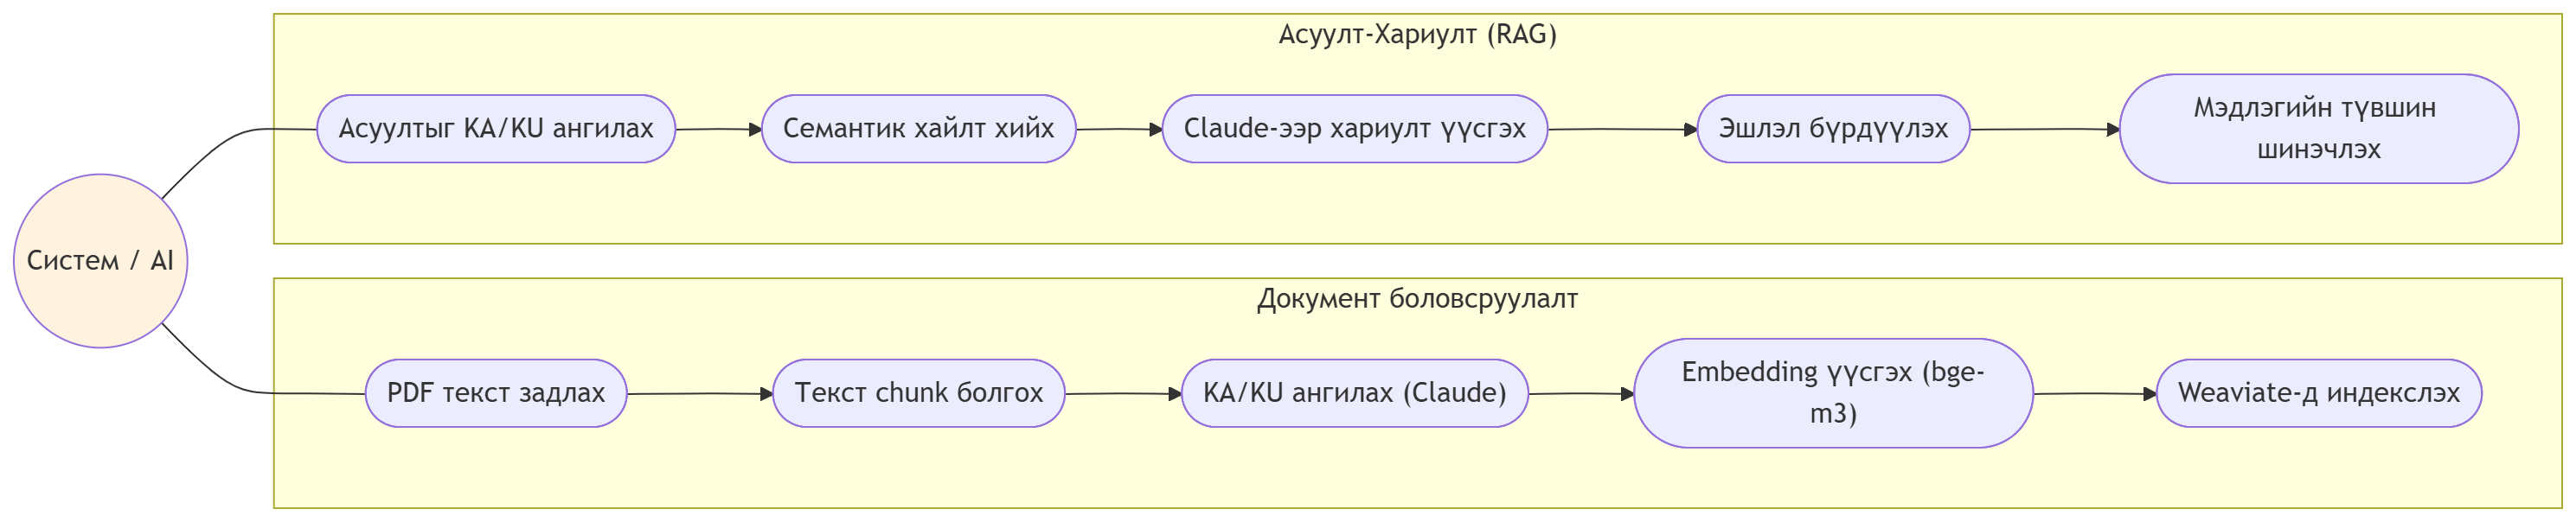
\includegraphics[width=0.8\textwidth,keepaspectratio]{assets/sys_use_case_diagram.png}
    \caption{Use case диаграмм}
    \label{fig:use_case_diagram}
\end{figure}


% ── 4-р бүлэг: Системийн архитектур ба дизайн ────────────────────────────────

\chapter{СИСТЕМИЙН АРХИТЕКТУР  БА \\ДИЗАЙН}

\section{Ерөнхий архитектурын диаграмм}

Энэхүү систем нь суралцагчийн оруулсан сургалтын материалыг боловсруулж, түүн дээр тулгуурлан асуултад эшлэлтэй хариулах, мөн суралцагчийн мэдлэгийн ахицыг \eng{mastery tracking} хэлбэрээр хадгалах зорилготой. Иймээс системийн архитектур нь ерөнхийдөө \eng{Frontend}, \eng{Backend API}, \eng{Document Processing Pipeline}, \eng{Vector Retrieval Layer}, \eng{Relational Database}, \eng{LLM/AI Layer} гэсэн үндсэн бүрэлдэхүүнээс тогтоно.

Системийн ажиллагааг ерөнхийд нь дараах байдлаар тайлбарлаж болно. Нэгдүгээрт, хэрэглэгч \eng{Frontend}-ээр дамжуулан \eng{PDF} эсвэл текст материал оруулна. Дараа нь \eng{Backend} болон \eng{worker pipeline} тухайн файлыг хадгалж, текстийг задлан \eng{document\_pages} болон \eng{document\_chunks} хэлбэрээр боловсруулна. Үүний дараа \eng{chunk}-уудын \eng{embedding} үүсч \eng{Weaviate} зэрэг \eng{Vector Database}-д индексжүүлэгдэнэ. Хэрэглэгч асуулт асуух үед систем холбогдох \eng{chunk}-уудыг retrieval хийж, тэдгээрийг \eng{LLM}-д контекст болгон дамжуулж, source-grounded хариулт үүсгэнэ. Гарсан хариултын эшлэлүүд \eng{message\_citations} хэлбэрээр хадгалагдана. \\ Үүнтэй зэрэгцэн асуулт, хариулт, эсвэл үнэлгээний үр дүнгээс шалтгаалан \eng{mastery\_evidence} бүртгэгдэж, \\ \eng{user\_ku\_mastery} болон \eng{user\_mastery} шинэчлэгдэнэ.

Иймээс энэхүү архитектур нь зөвхөн асуултад хариулах чат систем биш, харин \\сургалтын материалыг боловсруулах, хайх, тайлбарлах, эшлэл харуулах, суралцах ахицыг хянах нэгдсэн ухаалаг сургалтын туслах систем юм. Ялангуяа \eng{document\_chunks}-ийг retrieval-ийн үндсэн эх сурвалж болгон ашиглаж, эшлэл болон audit-ийг \eng{PostgreSQL} дээрх бүтэцтэй өгөгдөлтэй холбож байгаа нь системийн найдвартай байдлыг нэмэгдүүлдэг.

\subsection*{Ерөнхий архитектурын диаграмм}
\begin{figure}[H]
    \centering
    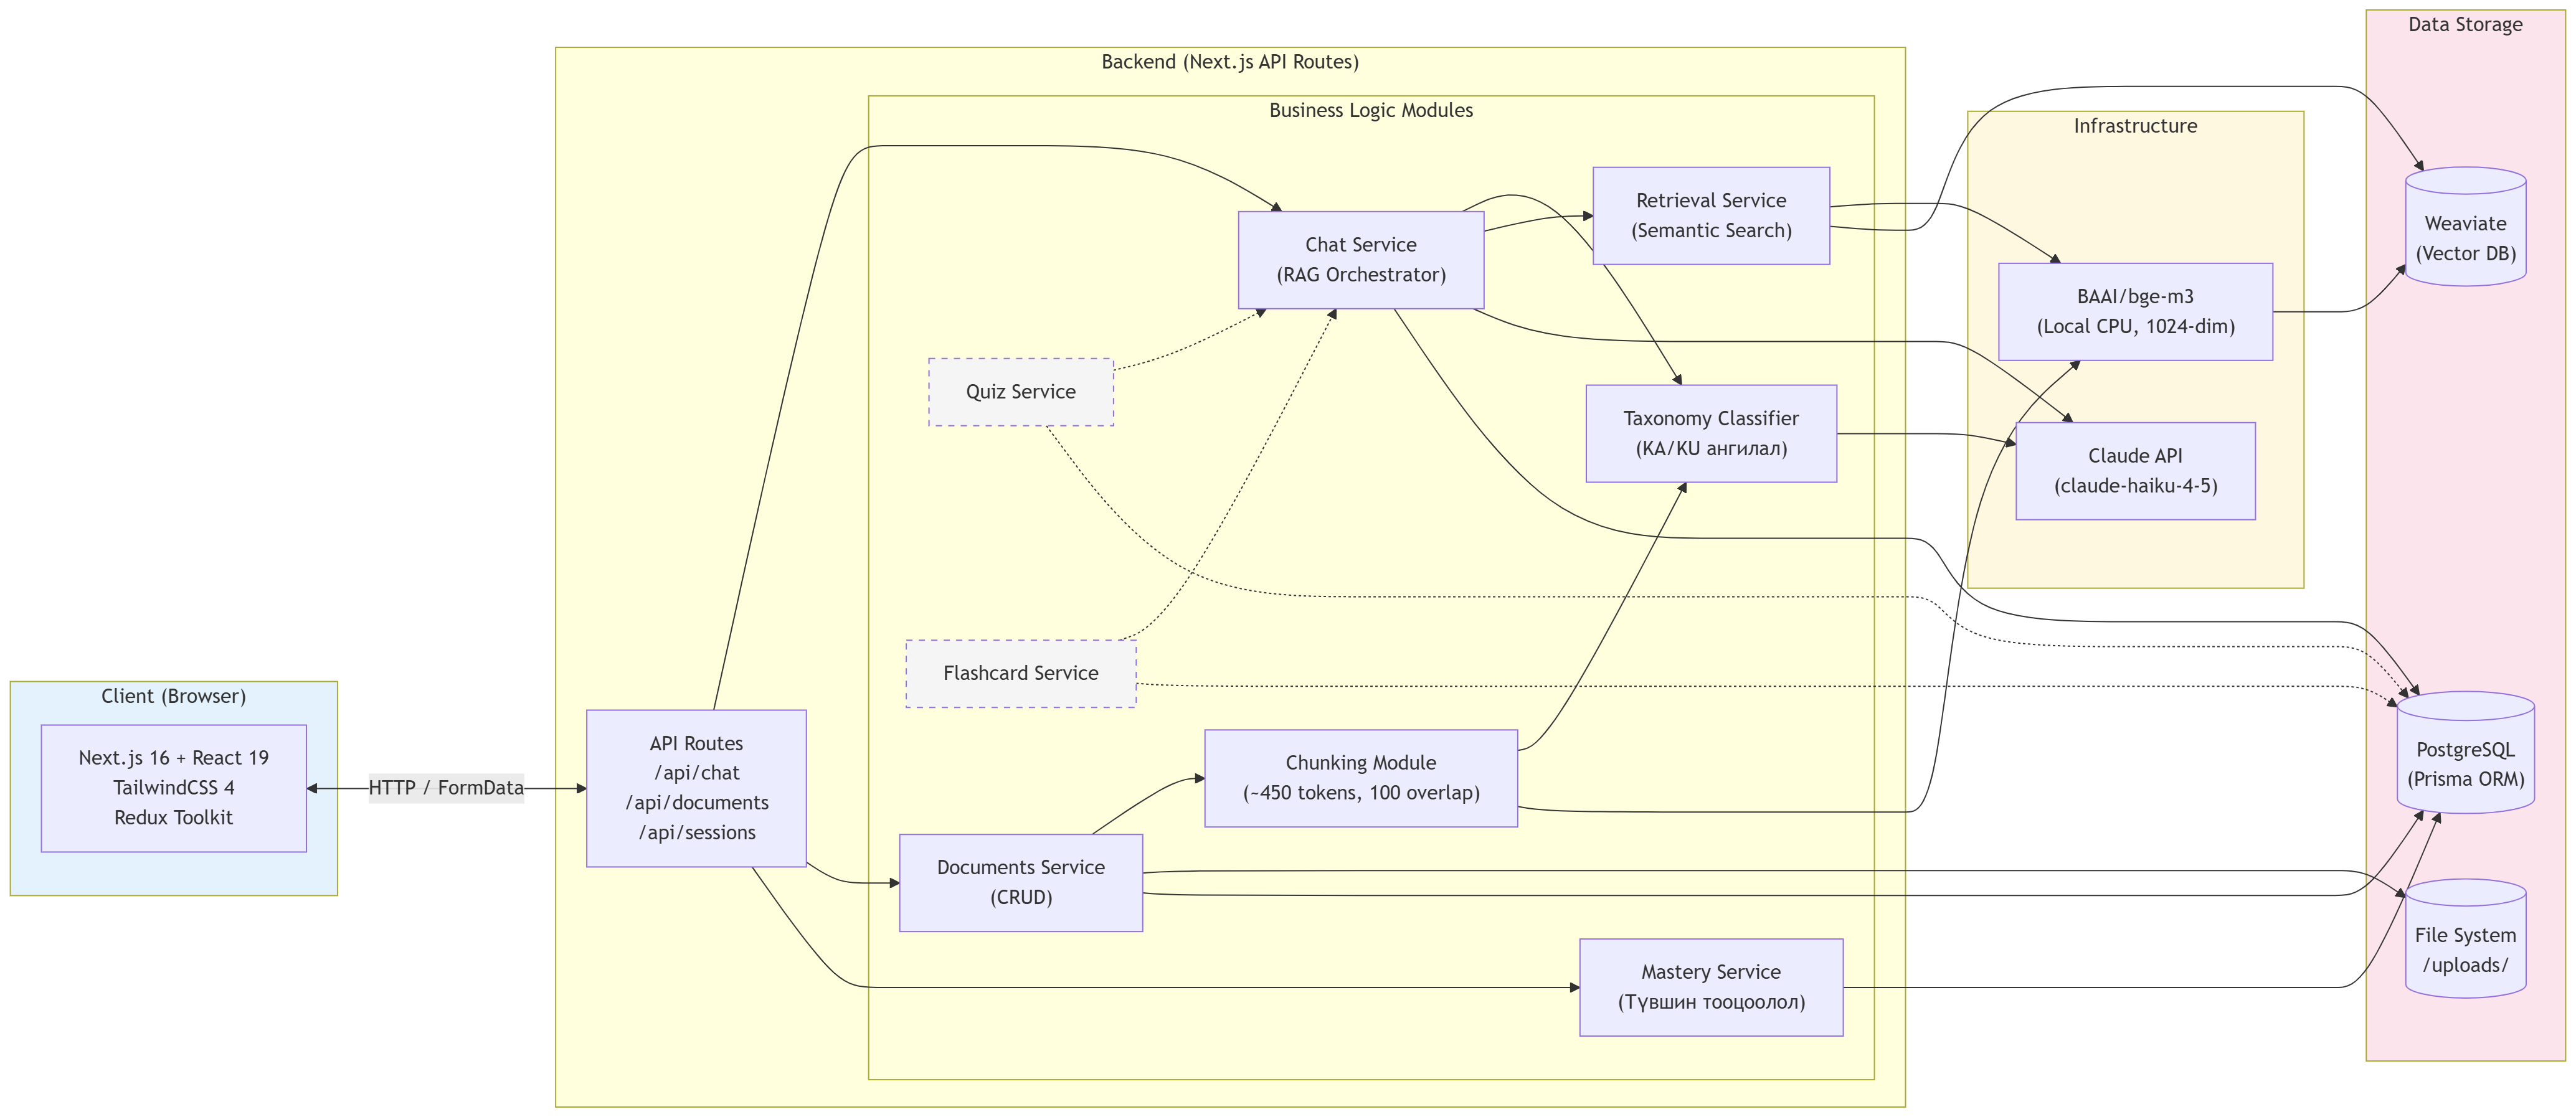
\includegraphics[width=1.1\textwidth,keepaspectratio]{assets/general_sys_arch.png}
    \caption{Ерөнхий архитектур диаграмм}
    \label{fig:general_architecture_diagram}
\end{figure}


\subsection*{Ерөнхий архитектурын тайлбар}

Дээрх архитектурт \eng{Frontend} нь хэрэглэгчээс асуулт авах, материал оруулах, эшлэл болон хянах самбар харуулах үүрэгтэй. \eng{Backend API} нь системийн үндсэн логикийг удирдаж, асуулт боловсруулах, retrieval хийх, \eng{taxonomy classification} хийх, \eng{mastery} шинэчлэх ажиллагааг хариуцна. \eng{Document Processing Pipeline} нь шинэ материал оруулах үед текст задлах, \eng{chunking} хийх, \eng{embedding} үүсгэхэд ашиглагдана. \eng{Vector Retrieval Layer} нь асуулттай утгын хувьд хамгийн ойролцоо эх сурвалжийн хэсгүүдийг хайж олно. Харин \eng{PostgreSQL Database} нь системийн \\ бүтэцтэй өгөгдөл, тухайлбал баримт бичиг, чат, эшлэл, \eng{mastery evidence} зэрэг мэдээллийг хадгална. \eng{LLM} нь retrieval-ээр олдсон контекстийг тайлбарлан ойлгомжтой хариулт үүсгэхэд ашиглагдана.

\section{Өгөгдлийн сангийн бүтэц (Хоорондын холбоо хамаарлын диаграмм)}

Системийн өгөгдлийн сан нь үндсэндээ дөрвөн логик давхаргад хуваагдана. Нэгдүгээрт, \eng{Curriculum/Taxonomy layer} нь \eng{domains}, \eng{knowledge\_areas}, \eng{knowledge\_units}, \eng{topics}, \eng{learning\_outcomes} зэрэг бүтэцтэйгээр сургалтын агуулгын шаталсан зохион байгуулалтыг хадгална. Хоёрдугаарт, \eng{User/Personalization layer} нь \eng{users}, \eng{user\_mastery}, \eng{user\_ku\_mastery}, \eng{mastery\_evidence}, \eng{quiz\_attempts}, \eng{flashcard\_attempts} зэрэг хүснэгтээр дамжин суралцагчийн ахиц болон personalization мэдээллийг хадгална. Гуравдугаарт, \eng{Document/RAG layer} нь \eng{documents}, \eng{document\_pages}, \eng{document\_chunks} гэсэн бүтэцтэйгээр эх сурвалжийн мэдээллийг хадгална. Дөрөвдүгээрт, \eng{Chat/Citation layer} нь \eng{chat\_sessions}, \eng{chat\_messages}, \eng{message\_citations}-аар дамжин хэрэглэгчийн харилцаа болон citation trace-ийг бүртгэнэ.

\eng{ER} түвшинд хамгийн чухал холбоонууд нь дараах байдалтай. \eng{domains} нь олон \eng{knowledge\_areas}-тай, \eng{knowledge\_areas} нь олон \eng{knowledge\_units}-тай, \eng{knowledge\_units} нь олон \eng{topics} болон \eng{learning\_outcomes}-той байна. \eng{users} нь олон \eng{documents}, \eng{chat\_sessions}, \eng{user\_mastery}, \eng{user\_ku\_mastery}, \eng{mastery\_evidence}, \\ \eng{quiz\_attempts}, \eng{flashcard\_attempts}-тай холбогдоно. \eng{documents} нь олон \eng{document\_pages} болон \\ \eng{document\_chunks}-тай; \eng{chat\_sessions} нь олон \eng{chat\_messages}-тай; \eng{chat\_messages} нь олон \eng{message\_citations}-тай холбогдоно. Мөн \eng{mastery\_evidence} нь \eng{user}, \eng{chat session}, \eng{message}, \eng{knowledge area}, \eng{knowledge unit}, optional байдлаар \eng{topic} болон \eng{learning outcome}-тай холбогдож байгаа нь personalization audit trail-ийг бүрдүүлдэг.

Энэ бүтэц нь гурван үндсэн зорилгыг зэрэг хангаж байна. Нэгдүгээрт, сургалтын taxonomy бүтэц хадгалах. Хоёрдугаарт, хэрэглэгчийн оруулсан эх сурвалж дээр retrieval ба citation хийх. Гуравдугаарт, personalization ба \eng{mastery progression}-ийг evidence-тэйгээр бүртгэх. Өөрөөр хэлбэл, уг \eng{ER} загвар нь зөвхөн өгөгдөл хадгалах схем биш, харин системийн сургалтын логикийг шууд тусгасан өгөгдлийн сангийн дизайн юм.

\subsection*{Хоорондын холбоо хамаарлын диаграммын mermaid код}
\begin{figure}[H]
    \centering
    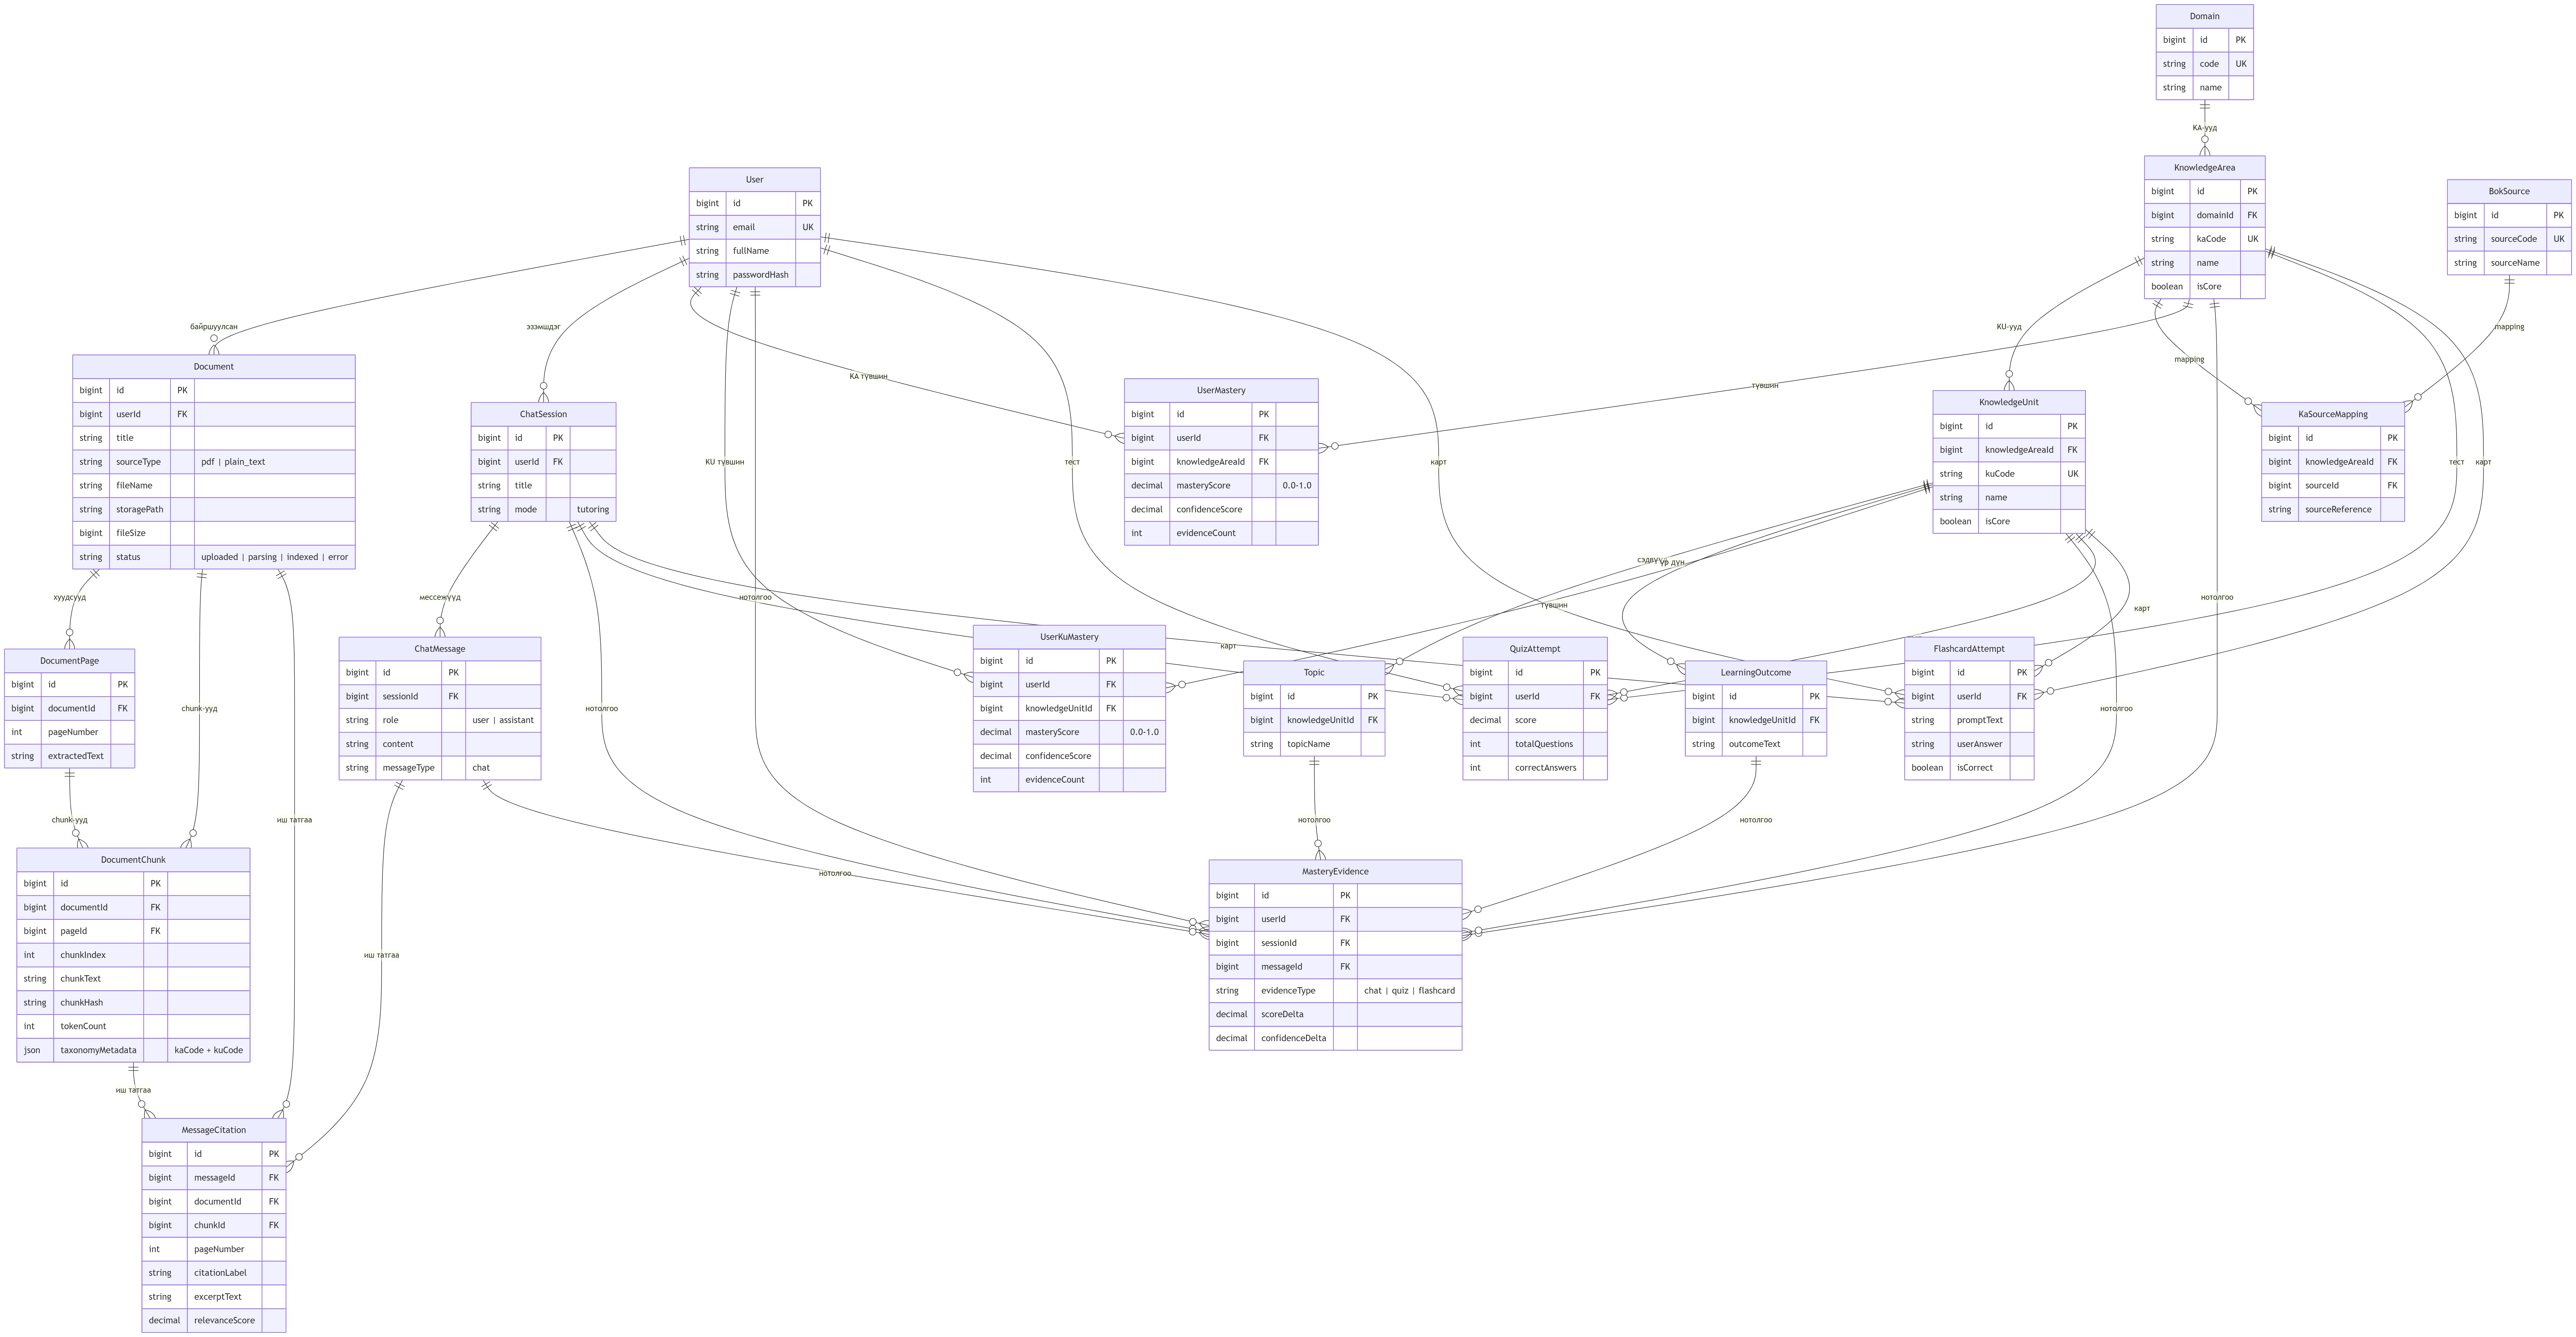
\includegraphics[width=1.1\textwidth,keepaspectratio]{assets/erd.png}
    \caption{ER диаграмм}
    \label{fig:er_diagram}
\end{figure}



\subsection*{Хоорондын холбоо хамаарлын диаграммын тайлбар}

\eng{domains → knowledge\_areas → knowledge\_units → topics / learning\_outcomes} холбоос нь сургалтын агуулгын шаталсан бүтцийг илэрхийлнэ. Энэ нь асуултыг \eng{KA/KU}-д ангилах, мөн суралцах ахицыг тодорхой агуулгын нэгж дээр хэмжих үндэс болдог.

\eng{users → documents → document\_pages / document\_chunks} бүтэц нь \eng{RAG source layer}-ийг бүрдүүлнэ. Хэрэглэгчийн оруулсан материал \eng{documents} хүснэгтэд бүртгэгдэж, дараа нь текст нь хуудас болон \eng{chunk} хэлбэрээр хуваагдан retrieval-д ашиглагдана.

\eng{users → chat\_sessions → chat\_messages → message\_citations} бүтэц нь чат харилцаа болон citation tracing-ийг хадгална. Ингэснээр ямар асуултад ямар эх сурвалж ашигласныг эргэн харах боломжтой болно.

\eng{users → user\_mastery / user\_ku\_mastery / mastery\_evidence} бүтэц нь personalization болон progress tracking-ийг илэрхийлнэ. \eng{user\_ku\_mastery} нь нарийвчилсан сэдвийн түвшний ахицыг, \eng{user\_mastery} нь \eng{knowledge area} түвшний нэгтгэсэн ахицыг хадгална. Харин \eng{mastery\_evidence} нь асуулт-хариулт, \eng{quiz}, \eng{flashcard} зэрэг үйл ажиллагаанаас ирсэн нотолгоог хадгалж, оноо шинэчлэх логикийн үндэс болно.

\eng{quiz\_attempts} болон \eng{flashcard\_attempts} хүснэгтүүд нь зөвхөн үнэлгээ хадгалах бус, мөн суралцагчийн мэдлэгийн түвшнийг шинэчлэх нэмэлт evidence эх үүсвэр болж өгнө. Иймээс ER бүтэц нь чат, retrieval, citation, personalization, assessment гэсэн бүх үндсэн дэд системийг нэг өгөгдлийн санд уялдуулж байна.

\section{API дизайн}

Энэхүү системийн \eng{API} нь \eng{Next.js App Router}-ийн \eng{route handler} хэлбэрээр хэрэгжсэн бөгөөд үндсэндээ \eng{authentication}, \eng{document management}, \eng{RAG chat}, \eng{session management}, \eng{mastery tracking}, \eng{quiz}, \eng{flashcard} гэсэн долоон дэд багцад хуваагдана. API-ийн дизайн хийхдээ дараах зарчмуудыг баримталсан. Үүнд: (i) хэрэглэгч тусгаарлалт (өөрийн өгөгдөлдөө л хандах), (ii) эх сурвалжтай хариултын мөрдөх чадвар, (iii) \eng{mastery} шинэчлэл нь үндсэн чат урсгалыг блоклохгүй байх, (iv) нэг endpoint нэг тодорхой үүрэгтэй байх зэрэг орно.

Нэвтрэлт ба эрхийн хяналт нь \eng{JWT cookie} дээр суурилсан. \eng{Register/Login} endpoint-ууд амжилттай дууссаны дараа \eng{auth\_token} нэртэй \eng{httpOnly} cookie үүсгэнэ. Дараагийн бүх хамгаалагдсан endpoint нь cookie-гээс хэрэглэгчийн \eng{userId}-г уншиж, өгөгдөлд хандах үед ownership шалгалт хийнэ. Иймд API түвшинд олон хэрэглэгчийн өгөгдөл хоорондоо холилдох эрсдэлийг бууруулж чадсан.

Хүснэгт \ref{tab:api-design-summary}-д Эхлэлийн түвшинд хэрэгжсэн endpoint-уудыг нэгтгэн үзүүлэв.

{\small
\setlength{\tabcolsep}{4pt}
\begin{longtable}{>{\raggedright\arraybackslash}p{4.0cm} >{\centering\arraybackslash}p{1.2cm} >{\raggedright\arraybackslash}p{5.2cm} >{\raggedright\arraybackslash}p{3.6cm}}
\caption{Системийн API endpoint-уудын нэгтгэл}\label{tab:api-design-summary}\\
\toprule
\textbf{Endpoint} & \textbf{Method} & \textbf{Үүрэг} & \textbf{Тайлбар} \\
\midrule
\endfirsthead
\toprule
\textbf{Endpoint} & \textbf{Method} & \textbf{Үүрэг} & \textbf{Тайлбар} \\
\midrule
\endhead
\bottomrule
\endfoot
\path{/api/auth/register} & POST & Шинэ хэрэглэгч бүртгэх & JWT cookie үүсгэнэ \\
\path{/api/auth/login} & POST & Нэвтрэлт хийх & JWT cookie үүсгэнэ \\
\path{/api/auth/logout} & POST & Гарах & Cookie устгана \\
\path{/api/auth/me} & GET & Идэвхтэй хэрэглэгч авах & Token шалгана \\
\path{/api/documents} & GET & Баримтын жагсаалт, шүүлт & q, type шүүлттэй \\
\path{/api/documents/upload} & POST & PDF/TXT оруулах, боловсруулах & Parse, Chunk, Classify, Index \\
\path{/api/documents/reclassify} & POST & Чанк дахин ангилах & Weaviate дахин индексжүүлнэ \\
\path{/api/documents/[id]} & GET & Нэг баримтын дэлгэрэнгүй авах & Ownership шалгана \\
\path{/api/documents/[id]} & DELETE & Нэг баримт устгах & Ownership шалгана \\
\path{/api/documents/[id]/file} & GET & Файлыг буцааж өгөх & Хадгалсан файлаас stream \\
\path{/api/chat} & POST & RAG хариулт үүсгэх & Citation болон mastery-тэй \\
\path{/api/sessions} & GET & Чатын сешнүүд авах & Хэрэглэгчээр шүүнэ \\
\path{/api/sessions/[id]} & GET & Сешний мессеж авах & Ownership шалгана \\
\path{/api/sessions/[id]} & DELETE & Сешн устгах & Ownership шалгана \\
\path{/api/mastery} & GET & KA/KU mastery авах & Dashboard өгөгдөл \\
\path{/api/quiz/generate} & POST & Тест үүсгэх & LLM + Retrieval \\
\path{/api/quiz/submit} & POST & Тест шалгах & Attempt + mastery evidence \\
\path{/api/flashcards/generate} & POST & Flashcard үүсгэх & LLM + Retrieval \\
\path{/api/flashcards/review} & POST & Flashcard үнэлэх & Attempt + mastery evidence \\
\end{longtable}
}

API-ийн өгөгдөл солилцооны хэлбэр нь endpoint-оос хамаарч өөр байна. Тухайлбал \eng{/api/chat} болон \eng{/api/documents/upload} нь \eng{multipart/form-data} ашигладаг бол бусад ихэнх endpoint \eng{JSON body} ашиглана. Энэ шийдэл нь файл дамжуулалт ба энгийн бизнес өгөгдлийн урсгалыг тусгаарлаж, фронтенд хөгжүүлэлтийн төвөгшлийг бууруулах давуу талтай.

Дүгнэж хэлбэл, энэхүү API дизайн нь RAG суурьтай сургалтын системийн үндсэн шаардлагууд болох баримт боловсруулах, эх сурвалжтай хариулах, personalization мэдээлэл хадгалах, хэрэглэгчийн ахицыг хэмжих процессуудыг нэг мөр, шалгагдах боломжтой интерфейсээр илэрхийлсэн.

\section{RAG Pipeline Flow}

Системийн асуулт-хариултын үндсэн урсгал нь \eng{POST /api/chat} endpoint-оор эхэлдэг. Хэрэглэгчийн асуулт орж ирмэгц систем эхлээд токеноор хэрэглэгчийг баталгаажуулж, шаардлагатай бол шинэ \eng{chat session} үүсгэнэ. Үүний дараа хэрэглэгчийн асуултыг \eng{chat\_messages} хүснэгтэд хадгалж, retrieval болон generation шат руу шилжинэ.

RAG урсгалын гол үе шатуудыг дараах байдлаар тодорхойлж болно.

\begin{enumerate}
    \item \textbf{Асуултын ангилал (KA/KU classification).} \\
    Асуултын текстийг \eng{Claude Haiku 4.5} загвараар ангилж, \eng{knowledge area} болон \eng{knowledge unit} код тодорхойлно. Энэ алхам нь retrieval-ийг зөв чиглүүлэх дохио болдог.

    \item \textbf{Семантик хайлт (vector retrieval).} \\
    Асуултыг \eng{BGE-M3} embedding загвараар вектор болгон хувиргаад \eng{Weaviate} дээр \eng{near-vector search} гүйцэтгэнэ. Эхний оролдлого нь KA-гаар шүүсэн хайлт; хэрэв хангалттай үр дүн өгөхгүй бол KA шүүлтгүй ерөнхий хайлт руу автоматаар шилждэг.

    \item \textbf{Контекст бүрдүүлэлт.} \\
    Олдсон дүнгээс чансаагаар нь хамгийн өндөр 4 чанк сонгож, баримтын нэр, хуудасны мэдээлэлтэй нь хамт \eng{system prompt} контекст болгон нэгтгэнэ.

    \item \textbf{Хариулт үүсгэх (grounded generation).} \\
    LLM нь зөвхөн тухайн контекстэд тулгуурлан хариулт үүсгэх бөгөөд [1], [2] гэх мэт ишлэлийн форматыг баримтална.

    \item \textbf{Citation бүртгэл.} \\
    Туслахын хариулттай холбоотой ишлэлүүдийг \eng{message\_citations} хүснэгтэд хадгална. Ингэснээр ямар хариулт аль баримтын ямар хуудсанд тулгуурсныг дараа нь шалгах боломж бүрдэнэ.

    \item \textbf{Mastery evidence шинэчлэл.} \\
    Хариулт, ишлэлийн чанарт тулгуурлан \eng{chat evidence} үүсгэж \eng{mastery} систем рүү дамжуулна. Энэ шинэчлэл амжилтгүй болсон ч чат хариултын урсгалыг зогсоохгүйгээр логлон өнгөрдөг.
\end{enumerate}

Хэрэв retrieval шатанд хэрэглэгчийн материал дотроос огт чанк олдохгүй бол систем "холбогдох мэдээлэл олдсонгүй" гэсэн аюулгүй fallback хариулт буцаана. Энэ нь эх сурвалжгүй таамаг хариулт (hallucination)-ыг багасгах чухал хамгаалалтын шийдэл юм.

Ийнхүү уг RAG pipeline нь зөвхөн хариулт үүсгэх төдий биш, харин ангилал, retrieval, citation trace, personalization шинэчлэлийг нэг урсгалд холбосон сургалтын зориулалттай шийдэл болж байна.

\section{Document Ingestion Pipeline}

Баримт оруулах урсгал нь \eng{POST /api/documents/upload} endpoint дээр хэрэгжсэн бөгөөд PDF эсвэл энгийн текст файлыг RAG-д ашиглахад бэлэн бүтцэд шилжүүлдэг. Энэхүү урсгал нь өгөгдлийн чанар, retrieval-ийн нарийвчлал, citation-ийн мөрдөх чадварыг зэрэг хангах зорилготой.

Ingestion pipeline-ийн алхмууд:

\begin{enumerate}
    \item \textbf{Файл байршуулах.} \\
    Систем зөвхөн PDF эсвэл TXT формат зөвшөөрч, файлыг \eng{uploads/} хавтсанд хадгална. Үүнтэй зэрэгцэн \eng{checksum} тооцож \eng{documents} хүснэгтэд мета өгөгдөл үүсгэнэ.

    \item \textbf{Parse ба page extraction.} \\
    PDF файлын хувьд \eng{unpdf} ашиглан хуудас бүрийн текстийг салгана; TXT файлын хувьд нэг хуудсын эх сурвалж гэж үзнэ. Гарсан үр дүнг \eng{document\_pages} хүснэгтэд хадгална.

    \item \textbf{Chunking.} \\
    Хуудасны текстийг үгийн түвшний гулсах цонхоор хуваана. Одоогийн хэрэгжүүлэлтэд default нь ойролцоогоор 338 үг/чанк, 75 үгийн давхцалтай. Энэ нь урт баримтад retrieval-ийн нарийвчлал ба контекстийн залгамж холбоог тэнцвэржүүлнэ.

    \item \textbf{Taxonomy classification.} \\
    Үүссэн чанк бүрийг LLM-ээр KA/KU ангилж, \eng{taxonomyMetadata}-д хадгална. Ингэснээр retrieval үед домайн дохиог ашиглах боломжтой болно.

    \item \textbf{Embedding.} \\
    Чанк текстүүдийг \eng{Xenova/bge-m3} embedding модел ашиглан 1024 хэмжээст вектор болгоно. Тооцооллыг batch хэлбэрээр хийх тул их хэмжээний баримтад үр ашигтай.

    \item \textbf{Vector indexing.} \\
    Вектор болон холбогдох мета өгөгдлийг \eng{Weaviate DocumentChunk} collection-д хадгална. Index амжилттай болсны дараа \eng{documents.status = indexed} болгон шинэчилнэ.
\end{enumerate}

Энэ урсгалд \eng{document\_chunks} хүснэгт болон Weaviate-д хадгалагдсан объектууд \eng{chunkId}-аар холбоотой байдаг. Иймд чат үеийн retrieval дүнгээс relational хүснэгт рүү буцаж citation үүсгэхэд \eng{traceability} алдагдахгүй.

Нэмж дурдахад \eng{/api/documents/reclassify} endpoint нь өмнө индексжүүлсэн баримтын чанк ангиллыг шинэ дүрмээр дахин тооцоолж, хуучин Weaviate объектуудыг устган шинэчилж индексжүүлэх зориулалттай. Энэ нь taxonomy сайжруулалтын дараах өгөгдлийн нийцлийг хангахад чухал.

\section{Mastery системийн дизайн}

Mastery дэд системийн зорилго нь суралцагчийн мэдлэгийг \eng{knowledge unit (KU)} түвшинд динамикаар үнэлж, түүнээс \eng{knowledge area (KA)} түвшний нэгтгэсэн төлөв гаргах явдал юм. Систем нь нэг удаагийн шалгалтын оноонд тулгуурлахгүй, харин олон төрлийн interaction-оос evidence цуглуулж тасралтгүй шинэчлэл хийх зарчим баримталдаг.

Архитектурын хувьд mastery нь гурван түвшний өгөгдөл дээр тогтоно.

\begin{itemize}
    \item \eng{mastery\_evidence}: event log (chat, quiz, flashcard-ийн нотолгоо)
    \item \eng{user\_ku\_mastery}: KU түвшний одоогийн оноо, confidence, evidence count
    \item \eng{user\_mastery}: KA түвшний нэгтгэсэн оноо
\end{itemize}

Оноо шинэчлэх үндсэн томьёо нь дараах байдлаар хэрэгжсэн.

\begin{equation}
S_{ku}^{new}=\max\left(0,\min\left(1, S_{ku}^{old}+\Delta_e\right)\right)
\end{equation}

энд $S_{ku}$ нь тухайн KU-ийн mastery score, $\Delta_e$ нь evidence төрлөөс хамаарах жин (эерэг эсвэл сөрөг) болно. Энэ томьёо нь score-ийг үргэлж $[0,1]$ мужид барина.

KA түвшний шинэчлэл нь тухайн KA-д харьяалагдах KU оноонуудын арифметик дундажаар тооцогдоно.

\begin{equation}
S_{ka}=\frac{1}{n}\sum_{i=1}^{n} S_{ku_i}
\end{equation}

Evidence жингийн хэрэгжсэн утгууд дараах байдалтай байна: \eng{chat\_correct}=+0.03, \eng{chat\_incorrect}=-0.02, \eng{flashcard\_correct}=+0.05, \eng{flashcard\_incorrect}=-0.02, \eng{quiz\_correct}=+0.08, \eng{quiz\_incorrect}=-0.03. Эдгээр утга нь formative interaction-уудын харьцангуй найдвартай байдлыг тусгаж, quiz-ийг хамгийн өндөр жинтэйгээр тооцож байна.

Mastery шинэчлэлийн урсгал нь дараах дарааллаар явагдана: (i) kuCode-оор KU-г resolve хийх, (ii) evidence event хадгалах, (iii) KU mastery upsert хийх, (iv) KA mastery recompute хийх. Энэ бүх алхам \eng{Prisma transaction}-ийн шаардлагагүйгээр нэг урсгалд хэрэгжсэн ч логикийн хувьд шалтгаант холбоо нь тодорхой тул audit хийхэд ойлгомжтой бүтэцтэй.

Иймээс уг дизайн нь personalization-ийг зөвхөн "статик оноо" биш, харин харилцан үйлчлэлийн түүх дээр суурилсан тасралтгүй үнэлгээ болгон хэрэгжүүлж, дараагийн шатны adaptive recommendation хөгжүүлэлтэд суурь өгөгдөл бүрдүүлж байна.


% ── 5-р бүлэг: Хэрэгжүүлэлтийн үр дүн ───────────────────────────────────────
\chapter{ХЭРЭГЖҮҮЛЭЛТИЙН ҮР ДҮН}

\section{Хөгжүүлэлтийн орчин}
Системийг веб суурьтай архитектураар хөгжүүлсэн. Frontend, backend, PostgreSQL өгөгдлийн сан, vector database, embedding model, large language model зэрэг үндсэн бүрэлдэхүүнүүдийг ашигласан. Энэ нь материалыг боловсруулах, семантик хайлт хийх, AI хариулт үүсгэх нөхцөлийг бүрдүүлсэн.

\begin{table}[H]
\centering
\caption{Системийн технологийн стек}
\label{tab:tech-stack}
\begin{tabularx}{\textwidth}{>{\raggedright\arraybackslash}p{3.2cm} >{\raggedright\arraybackslash}p{5.2cm} >{\raggedright\arraybackslash}X}
\toprule
\textbf{Бүрэлдэхүүн} & \textbf{Ашигласан технологи} & \textbf{Зориулалт} \\
\midrule
Frontend & Next.js / React / TypeScript & Хэрэглэгчийн интерфейс \\
Backend & Node.js / NestJS / Express & API болон бизнес логик \\
Relational DB & PostgreSQL & Metadata, user, session, mastery \\
Vector DB & Weaviate  & Embedding хадгалалт ба semantic search \\
Embedding model & BGE-M3 & Query болон chunk embedding \\
LLM & Claude API & Хариулт үүсгэх \\
File processing & PDF parser module & PDF-с текст задлах \\
Version control & Git / GitHub & Кодын хувилбар удирдлага \\
\bottomrule
\end{tabularx}
\end{table}

\begin{figure}[H]
    \centering
    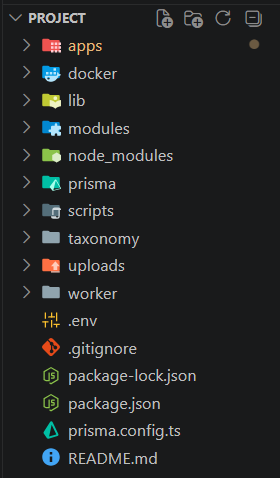
\includegraphics[width=0.3\textwidth,keepaspectratio]{assets/project_structure.png}
    \caption{pgAdmin дээрх database schema screenshot}
    \label{fig:use_case_diagram}
\end{figure}

\begin{figure}[H]
    \centering
    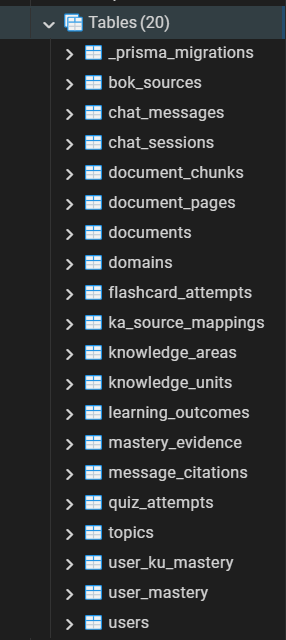
\includegraphics[width=0.3\textwidth,keepaspectratio]{assets/pgadmin_tables.png}
    \caption{Системийн файлын үндсэн бүтэц}
    \label{fig:use_case_diagram}
\end{figure}
\begin{figure}[H]
    \centering
    
\includegraphics[width=1.1\textwidth,keepaspectratio]{assets/weaviate_docker.png}
    \caption{Докер дээрх контейнор}
    \label{fig:use_case_diagram}
\end{figure}
\begin{figure}[H]
    \centering
    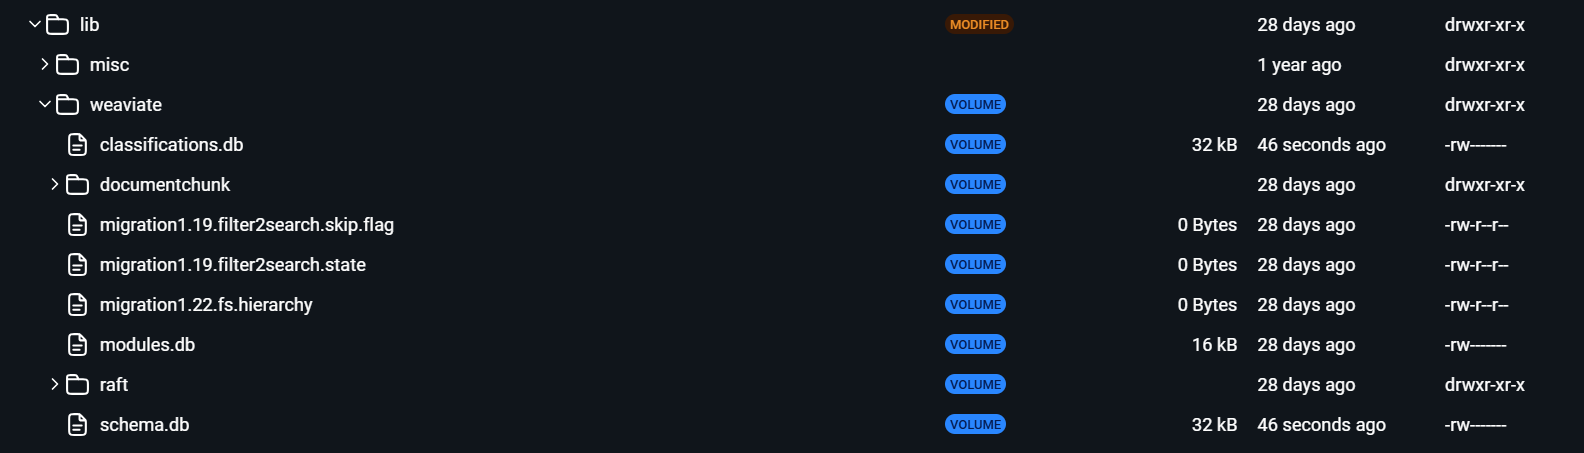
\includegraphics[width=0.8\textwidth,keepaspectratio]{assets/docker_file_structure.png}
    \caption{Weaviate-ийн вектор өгөгдлийн сангийн бүтэц}
    \label{fig:use_case_diagram}
\end{figure}


\section{Гол модулиудын хэрэгжүүлэлт}

\subsection{Ingestion pipeline}
Энэ модуль нь хэрэглэгчийн оруулсан PDF файлыг хүлээн авч, текстийг задлан, chunk болгон хувааж, embedding үүсгэн өгөгдлийн санд хадгална. Уг процесс нь дараагийн retrieval шатны суурь болдог.

\begin{figure}[H]
    \centering
    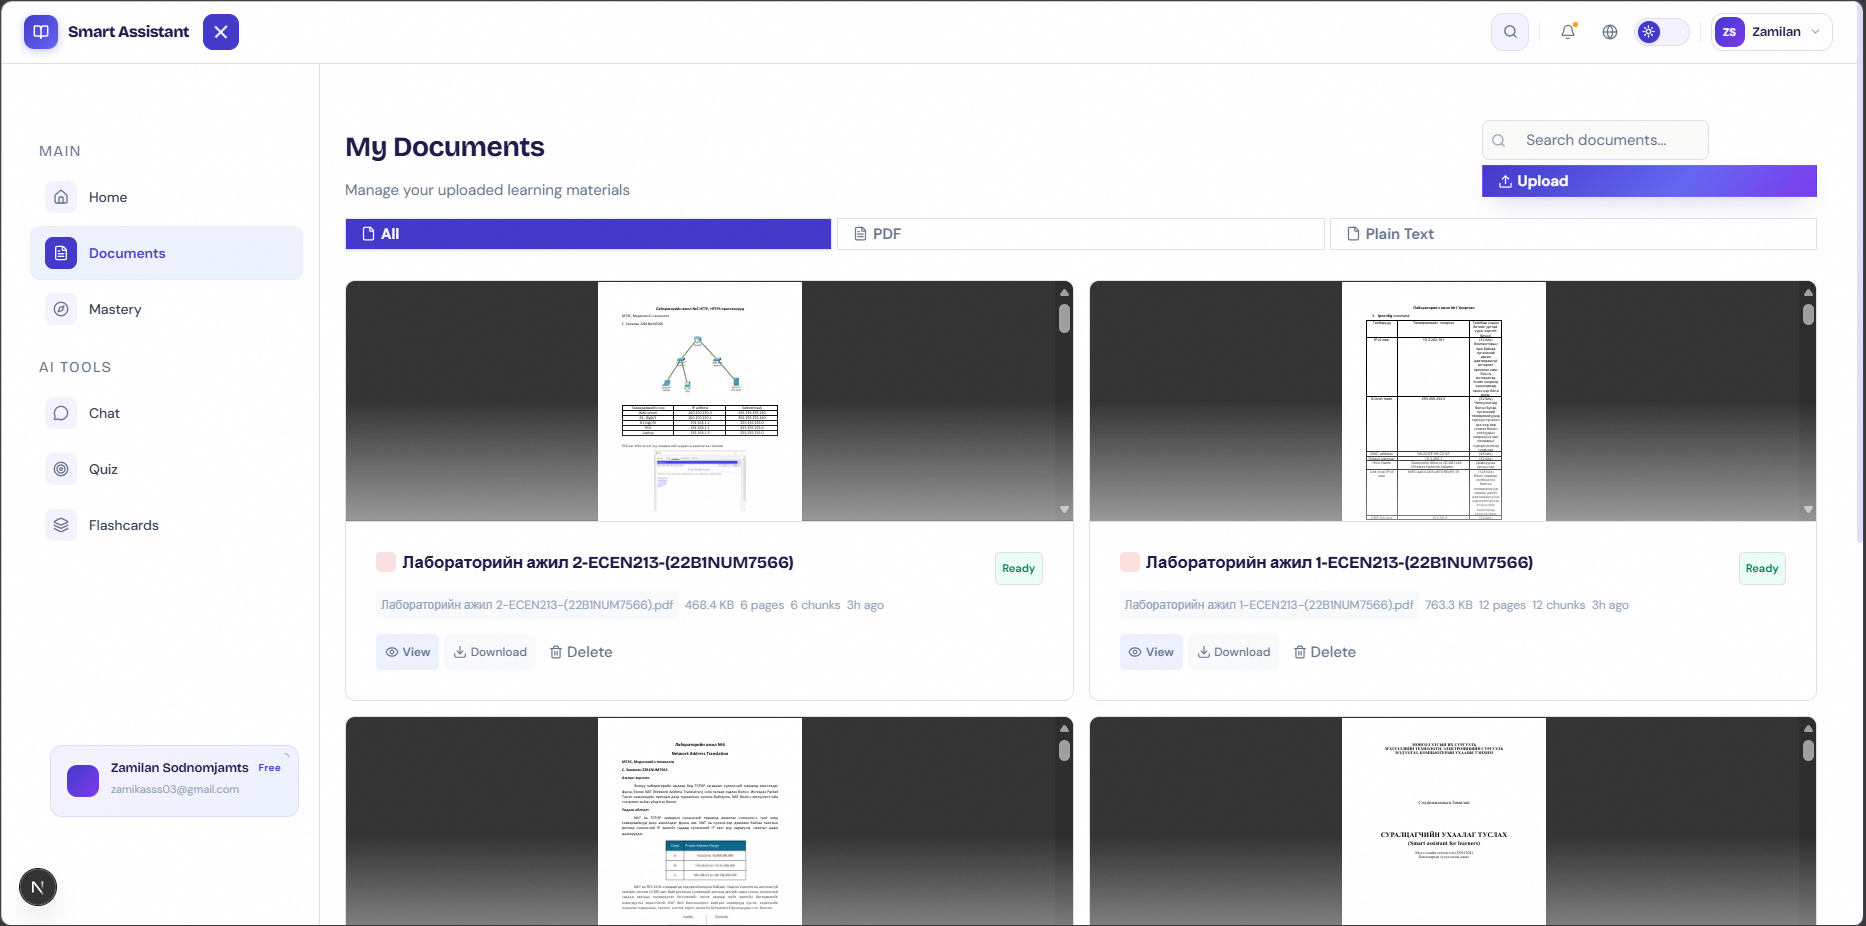
\includegraphics[width=0.8\textwidth,keepaspectratio]{assets/documents_page.png}
    \caption{Баримт бичиг хуудас/PDF upload интерфейс}
    \label{fig:documents_page}
\end{figure}
Энэхүү дэлгэцээр хэрэглэгч сургалтын материалыг PDF хэлбэрээр системд оруулна. Файл сонгогдсоны дараа upload үйлдэл эхэлж, backend талд ingestion pipeline ажиллана.
\begin{figure}[H]
    \centering
    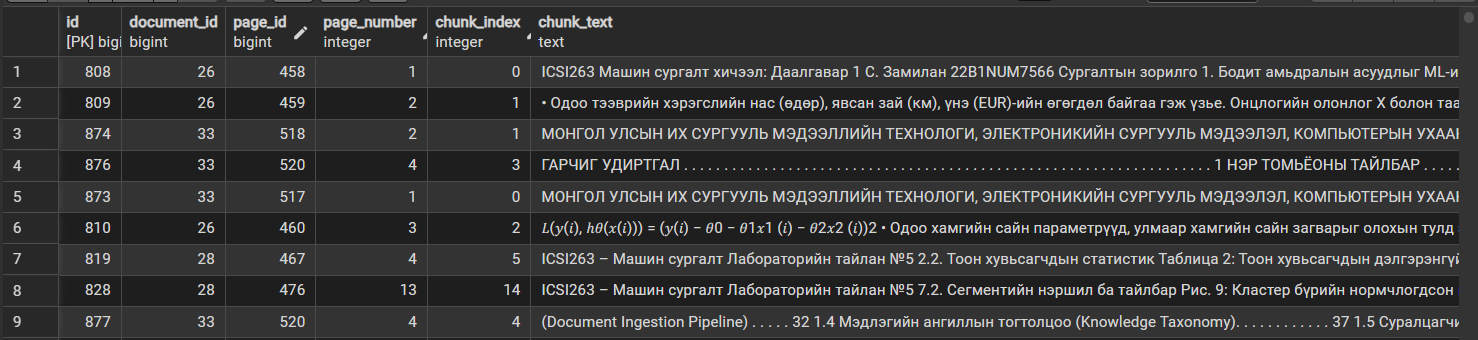
\includegraphics[width=1.0\textwidth,keepaspectratio]{assets/doc_chunks_table.png}
    \caption{pgadmin дээрх document chunks хүснэгт}
    \label{fig:doc_chunks_table}
\end{figure}
\begin{figure}[H]
    \centering
    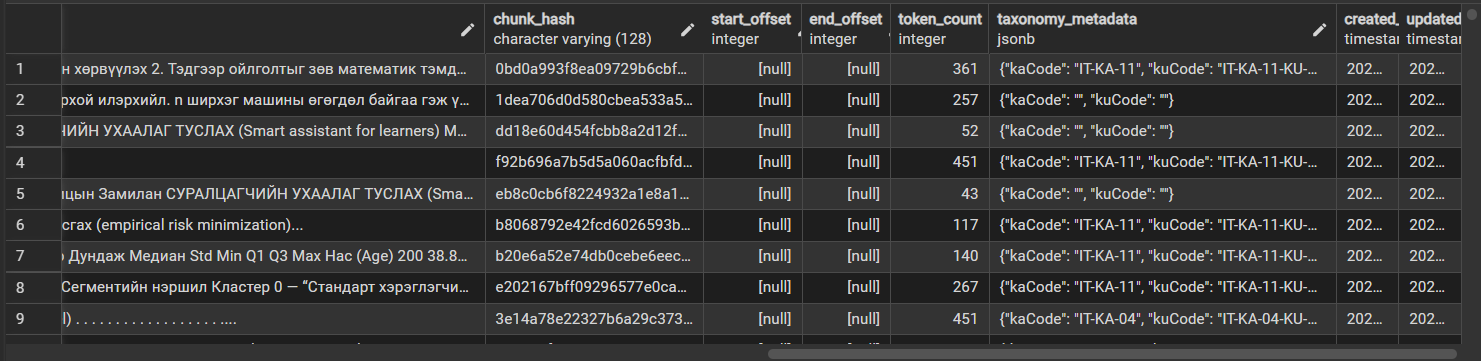
\includegraphics[width=0.9\textwidth,keepaspectratio]{assets/doc_chunks_table_2.png}
    \caption{Мета дата хадгалсан байдал}
    \label{fig:doc_chunks_table2}
\end{figure}
\subsection{RAG pipeline}
Энэ модуль нь хэрэглэгчийн оруулсан PDF файлыг хүлээн авч, текстийг задлан, chunk болгон хувааж, embedding үүсгэн өгөгдлийн санд хадгална. Уг процесс нь дараагийн retrieval шатны суурь болдог.

\begin{figure}[H]
    \centering
    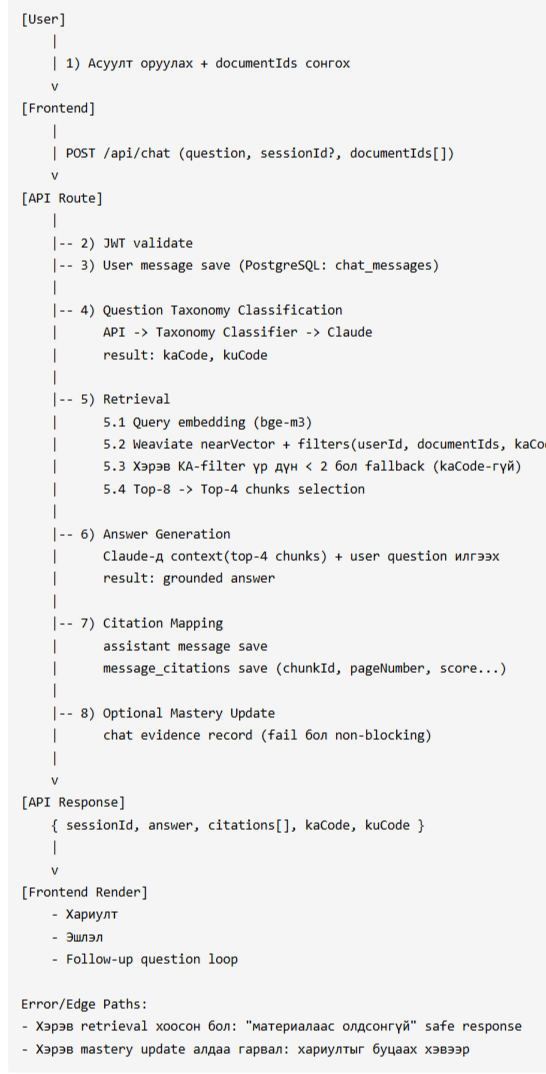
\includegraphics[width=0.6\textwidth,keepaspectratio]{assets/rag_pipeline.png}
    \caption{rag pipeline}
    \label{fig:rag_pipeline}
\end{figure}


\subsection{Taxonomy classification}
Энэ модуль нь асуултыг агуулга, зорилгын дагуу ангилна. Ангиллын үр дүн нь системийн хариултын хэлбэр болон тайлбарын түвшинг тохируулахад ашиглагдана. 
\begin{figure}[H]
    \centering
    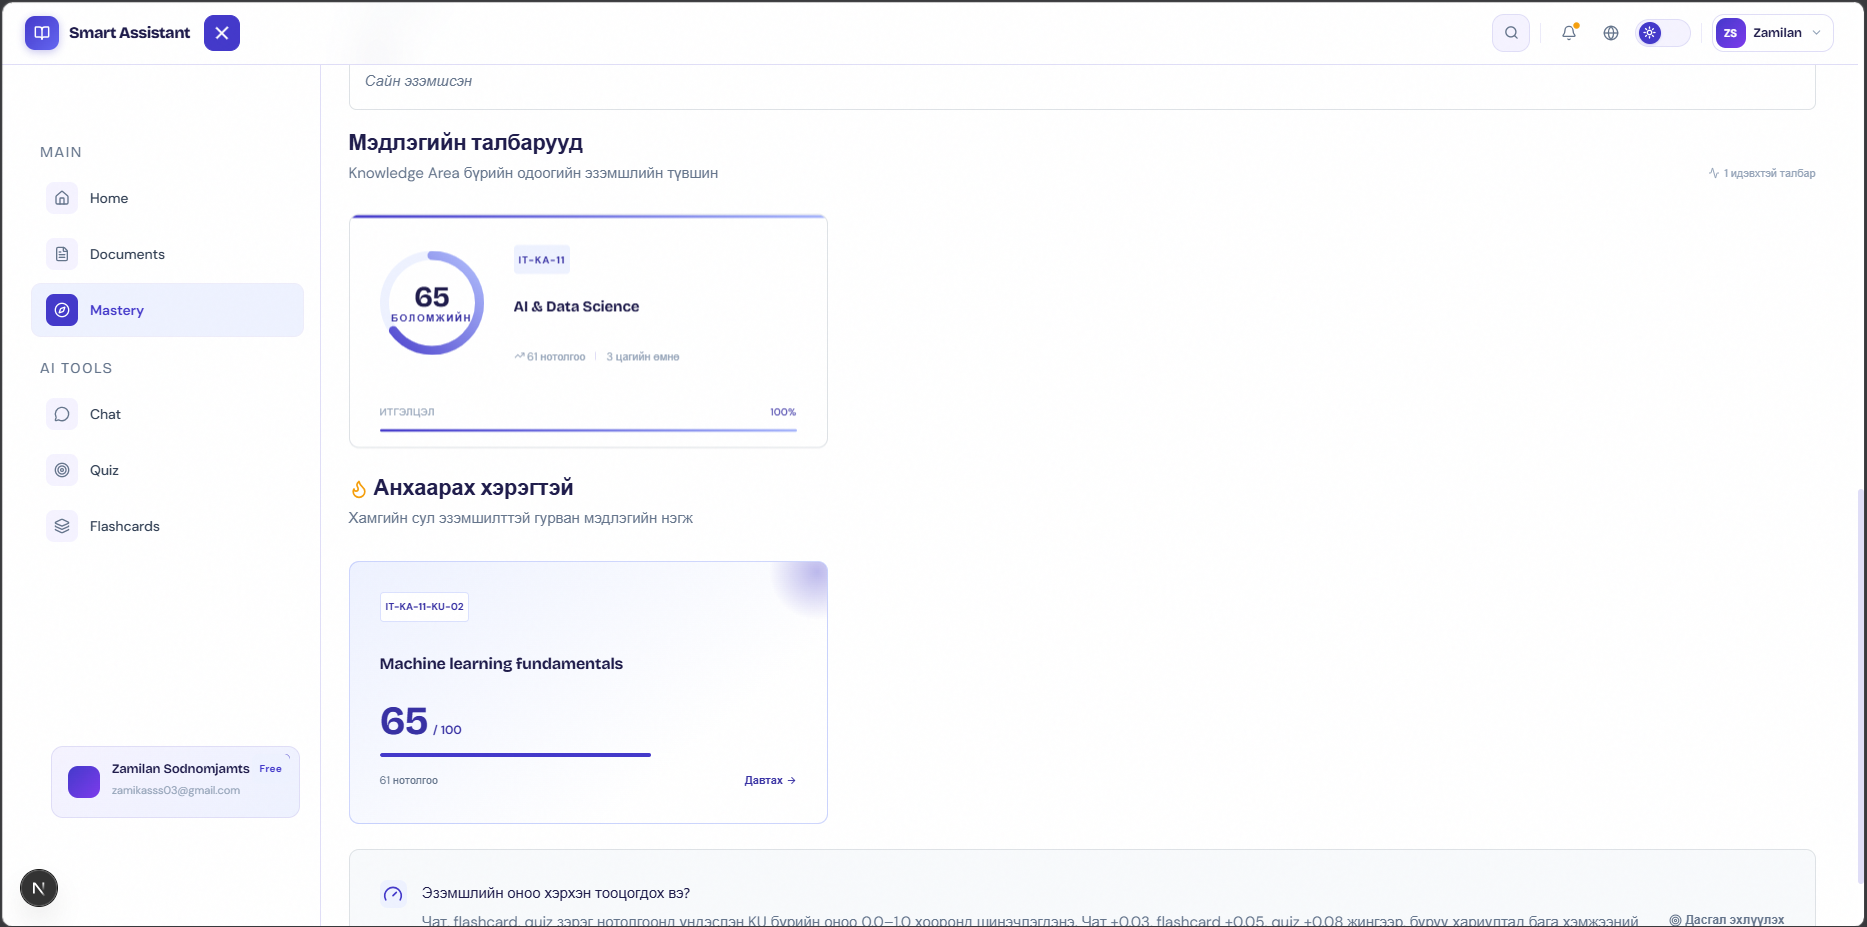
\includegraphics[width=1.0\textwidth,keepaspectratio]{assets/mastery_page2.png}
    \caption{Mastery хуудас дээрх KA, KU}
    \label{fig:mastery_page2}
\end{figure}

\subsection{Mastery update}
Энэ модуль нь хэрэглэгчийн асуулт, харилцан үйлчлэлд үндэслэн тухайн сэдвийн эзэмшлийн түвшинг шинэчилнэ. Ингэснээр суралцагчийн ахиц, хувьчилсан зөвлөмжийг гаргах боломж бүрдэнэ.

\begin{figure}[H]
    \centering
    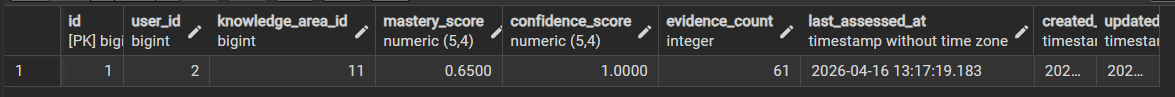
\includegraphics[width=1.0\textwidth,keepaspectratio]{assets/user_mastery_table.png}
    \caption{pgadmin дээрх хэрэглэгчийн mastery хүснэгт}
    \label{fig:user_mastery_table}
\end{figure}
\begin{figure}[H]
    \centering
    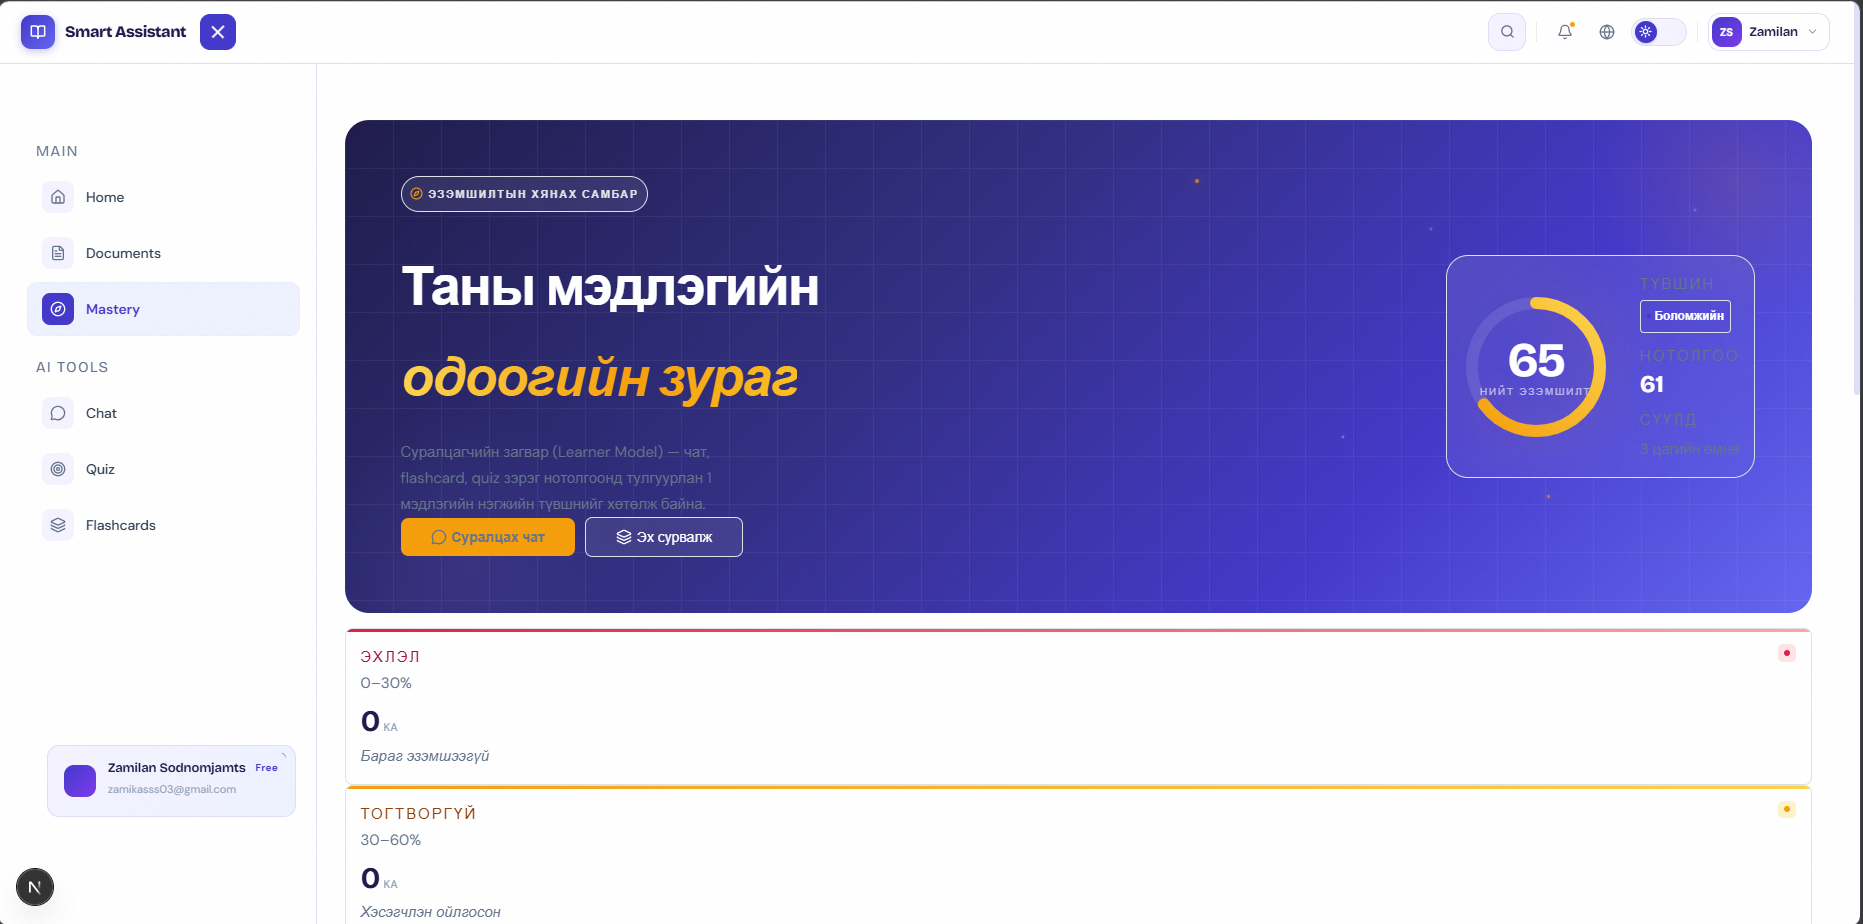
\includegraphics[width=1.0\textwidth,keepaspectratio]{assets/mastery_page.png}
    \caption{Mastery хуудас}
    \label{fig:mastery_page}
\end{figure}

\section{Дэлгэцийн зураг (UI screenshots)}
\begin{figure}[H]
    \centering
    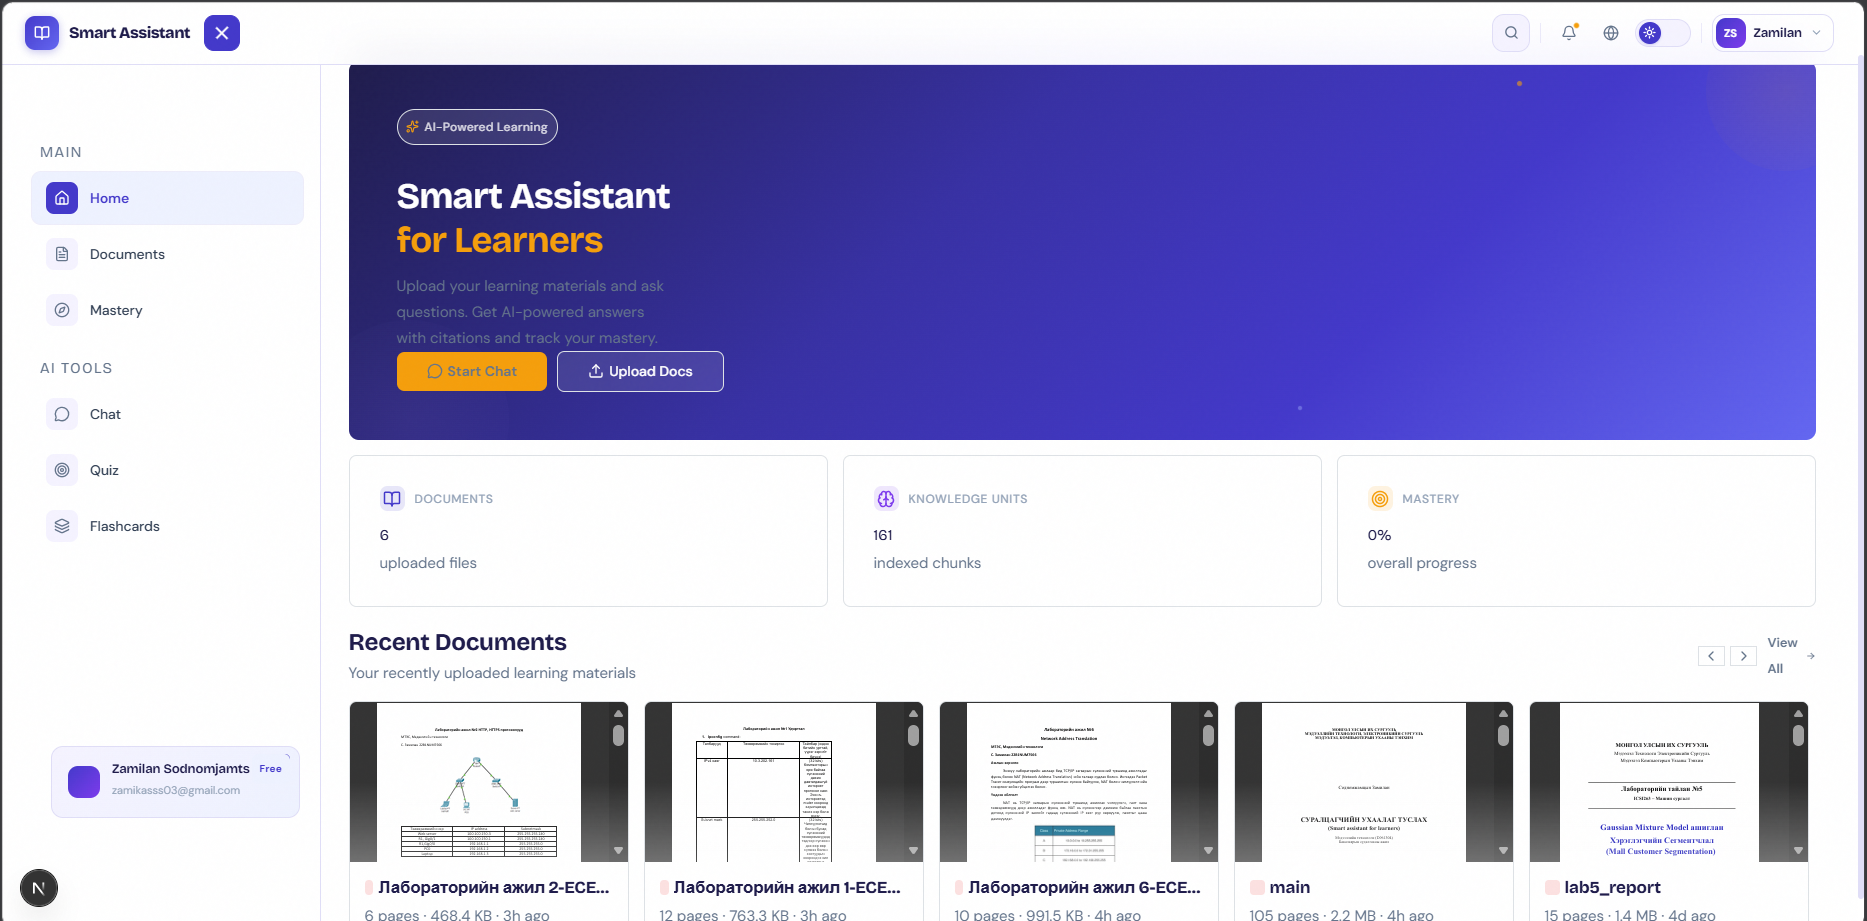
\includegraphics[width=1.0\textwidth,keepaspectratio]{assets/home_page.png}
    \caption{Нүүр хуудас}
    \label{fig:home_page}
\end{figure}

\begin{figure}[H]
    \centering
    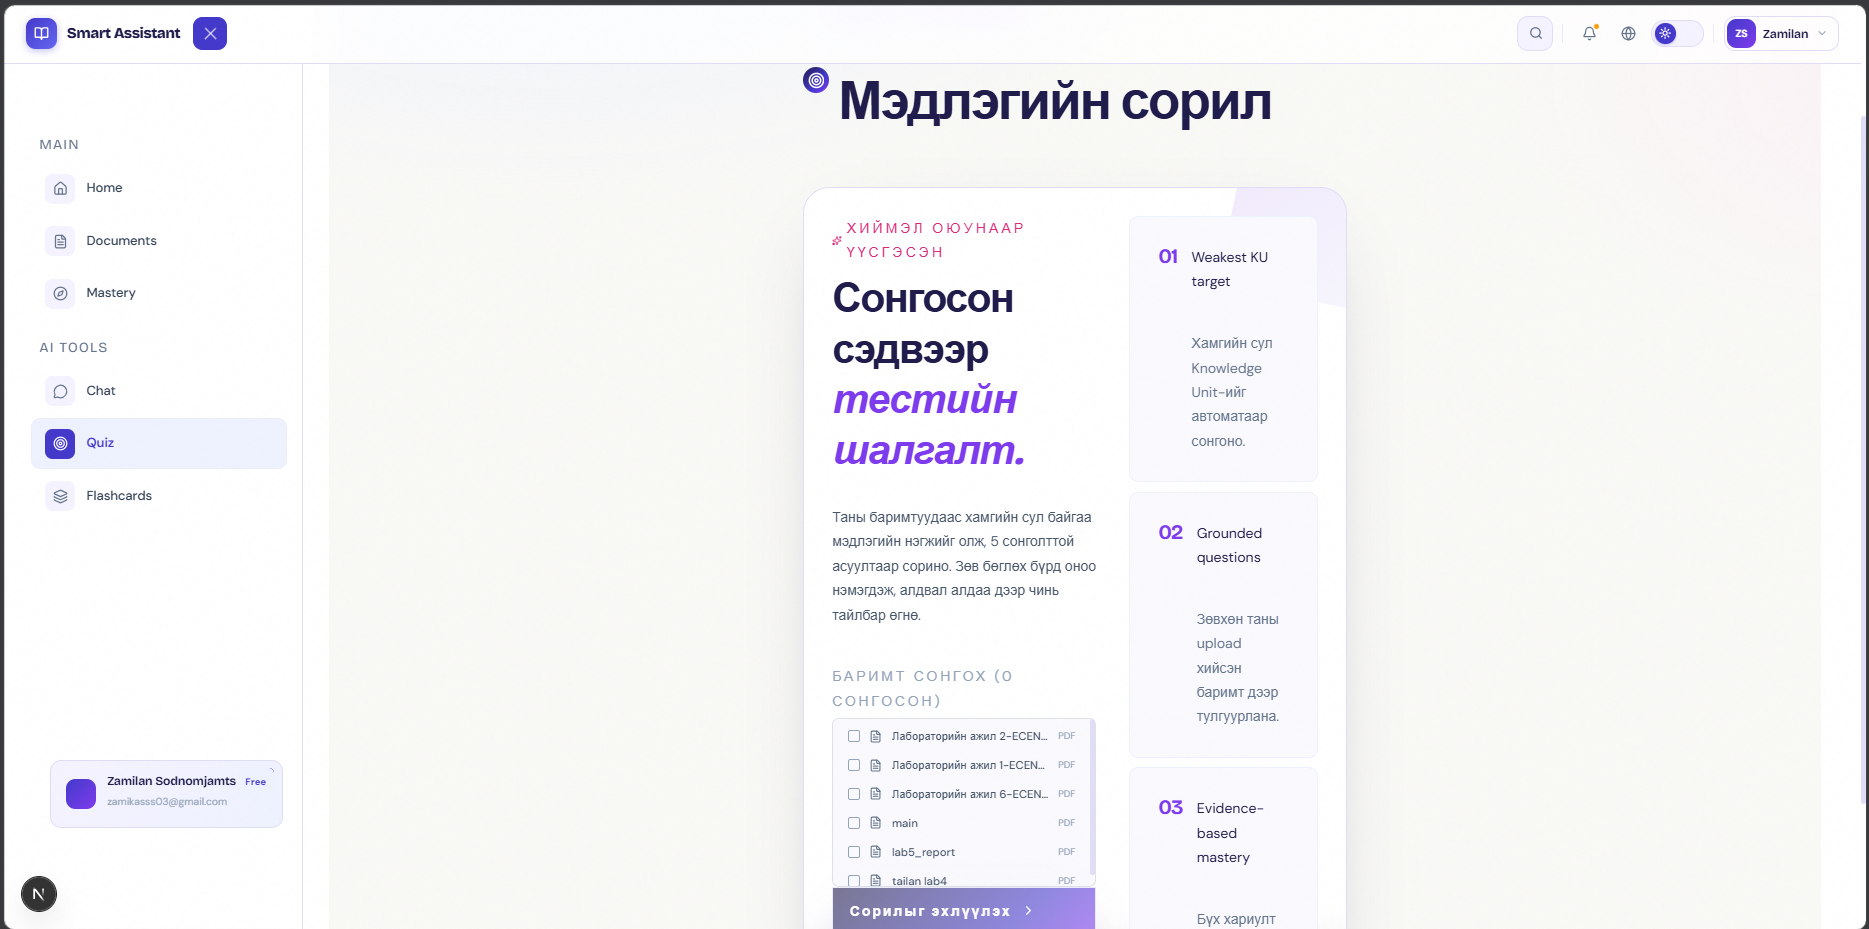
\includegraphics[width=1.0\textwidth,keepaspectratio]{assets/quiz_page.png}
    \caption{Шалгалтын хуудас}
    \label{fig:quiz_page}
\end{figure}
\begin{figure}[H]
    \centering
    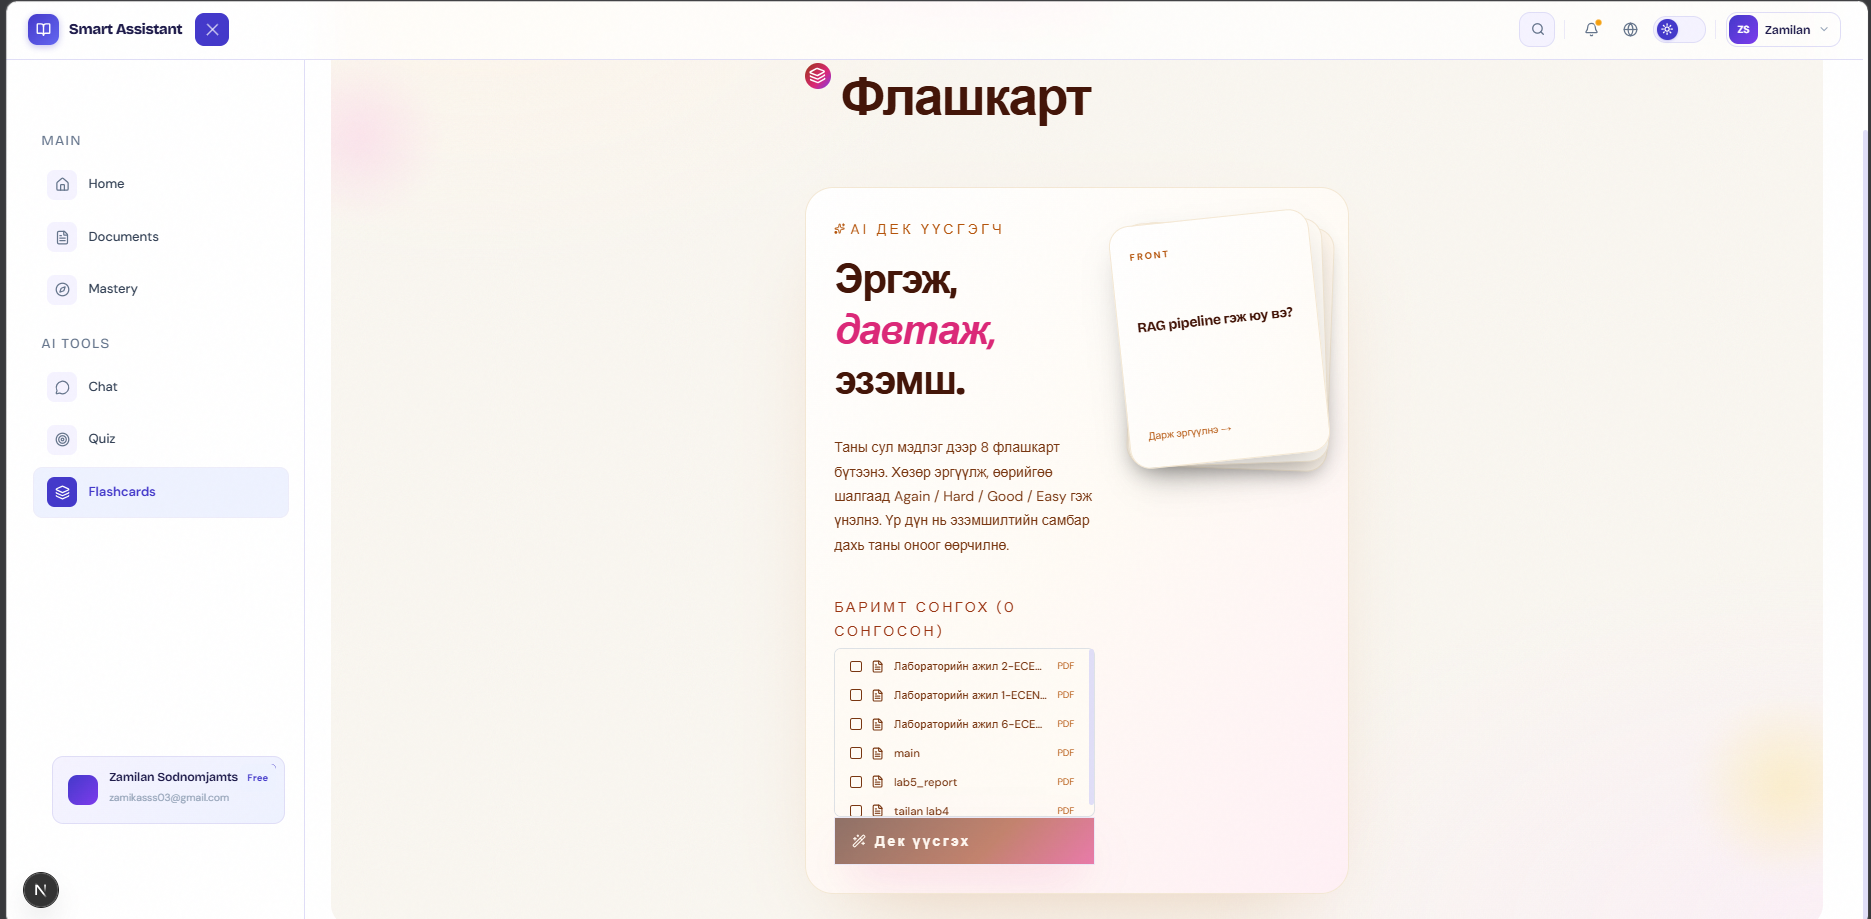
\includegraphics[width=1.0\textwidth,keepaspectratio]{assets/flashcard_page.png}
    \caption{Карт хуудас}
    \label{fig:flashcard_page}
\end{figure}
% ── 6-р бүлэг: Турших, тестлэх ───────────────────────────────────────────────
\chapter{ТУРШИХ, ТЕСТЛЭХ}

\section{Тестийн стратеги}

\section{Хариултын нарийвчлалын тест}

\section{Гүйцэтгэлийн тест}

\section{Хэрэглэгчийн санал асуулга}


% ── Дүгнэлт ───────────────────────────────────────────────────────────────────
\newgeometry{left=3cm,right=3cm,top=2.5cm,bottom=2cm,includefoot}

\superchapter{ДҮГНЭЛТ}


% ── Ном зүй ───────────────────────────────────────────────────────────────────
\newgeometry{left=3cm,right=3cm,top=2.5cm,bottom=2cm,includefoot}

\renewcommand{\bibname}{\begin{center}\textbf{НОМ ЗҮЙ}\end{center}}
\addcontentsline{toc}{part}{НОМ ЗҮЙ}

\begin{thebibliography}{}

\bibitem{alkhatlan2018}
Alkhatlan, A., \& Kalita, J. (2018).
Intelligent Tutoring Systems: A Comprehensive Historical Survey with Recent Developments.
\textit{International Journal of Computer Applications}, 181(43), 1--20.

\bibitem{xu2021}
Xu, Z., Zhao, Y., Liew, J., \& Pang, X. (2021).
Evolution and trends in intelligent tutoring systems research: a multidisciplinary and scientometric view.
\textit{Asia Pacific Education Review}, 22, 441--461.

\bibitem{carbonell1970}
Carbonell, J. (1970).
AI in CAI: An artificial-intelligence approach to computer-assisted instruction.
\textit{IEEE Transactions on Man-Machine Systems}, 11(4), 190--202.

\bibitem{bloom1984}
Bloom, B. S. (1984).
The 2 sigma problem: The search for methods of group instruction as effective as one-to-one tutoring.
\textit{Educational Researcher}, 13(6), 4--16.

\bibitem{vanlehn2011}
VanLehn, K. (2011).
The relative effectiveness of human tutoring, intelligent tutoring systems, and other tutoring systems.
\textit{Educational Psychologist}, 46(4), 197--221.

\bibitem{freedman2000}
Freedman, R. (2000).
What is an intelligent tutoring system?
\textit{Intelligence}, 11(3), 15--16.

\bibitem{sciencedirect2024}
Nkambou, R., Bourdeau, J., \& Mizoguchi, R. (Eds.). (2010).
\textit{Advances in Intelligent Tutoring Systems}. Springer.

\bibitem{liu2025}
Liu, Z., Agrawal, P., Singhal, S., Madaan, V., Kumar, M., \& Verma, P. K. (2025).
LPITutor: an LLM based personalized intelligent tutoring system using RAG and prompt engineering.
\textit{PeerJ Computer Science}, 11, e2991.

\bibitem{karran2025}
Karran, J. A., Boasen, J., \& Léger, P. M. (2025).
A systematic review of AI-driven intelligent tutoring systems (ITS) in K-12 education.
\textit{npj Science of Learning}, 10, 29.

\bibitem{lewis2020}
Lewis, P., Perez, E., Piktus, A., Petroni, F., Karpukhin, V., Goyal, N., \ldots{} \& Kiela, D. (2020).
Retrieval-Augmented Generation for Knowledge-Intensive NLP Tasks.
\textit{Advances in Neural Information Processing Systems}, 33, 9459--9474.

\bibitem{gao2024}
Gao, Y., Xiong, Y., Gao, X., Jia, K., Pan, J., Bi, Y., \ldots{} \& Wang, H. (2024).
Retrieval-Augmented Generation for Large Language Models: A Survey.
\textit{arXiv preprint arXiv:2312.10997v5}.

\bibitem{springer2025}
Springer. (2025).
Retrieval-Augmented Generation (RAG).
\textit{Business \& Information Systems Engineering}.
DOI: 10.1007/s12599-025-00945-3.

\bibitem{nature2025}
Thesen, T. et al. (2025).
A generative AI teaching assistant for personalized learning in medical education.
\textit{npj Digital Medicine}.

\bibitem{mdpi2025}
MDPI. (2025).
Developing a Local Generative AI Teaching Assistant System: Utilizing Retrieval-Augmented Generation Technology.
\textit{Electronics}, 14(17), 3402.

\bibitem{devto2026}
Giggs, D. R. (2026).
RAG Pipeline Deep Dive: Ingestion, Chunking, Embedding, and Vector Search.
\textit{DEV Community}.

\bibitem{dhiwise2025}
DHIwise. (2025).
Complete Guide to Building a Robust RAG Pipeline 2025.

\bibitem{databricks2025}
Databricks. (2025).
Build an unstructured data pipeline for RAG.

\bibitem{firecrawl2025}
Firecrawl. (2025).
Best Chunking Strategies for RAG in 2025.

\bibitem{langcopilot2025}
LLM Practical Experience Hub. (2025).
Document Chunking for RAG: 9 Strategies Tested.

\bibitem{chen2024}
Chen, J., Xiao, S., Zhang, P., Luo, K., Lian, D., \& Liu, Z. (2024).
BGE M3-Embedding: Multi-Lingual, Multi-Functionality, Multi-Granularity Text Embeddings Through Self-Knowledge Distillation.
\textit{ACL Findings 2024}, 2318--2335.

\bibitem{bloom1956}
Bloom, B. S., Engelhart, M. D., Furst, E. J., Hill, W. H., \& Krathwohl, D. R. (1956).
\textit{Taxonomy of Educational Objectives: The Classification of Educational Goals. Handbook 1: Cognitive Domain.}
New York: David McKay Company.

\bibitem{anderson2001}
Anderson, L. W., \& Krathwohl, D. R. (Eds.). (2001).
\textit{A Taxonomy for Learning, Teaching, and Assessing: A Revision of Bloom's Taxonomy of Educational Objectives.}
New York: Longman.

\bibitem{cs2023}
ACM, IEEE-CS, \& AAAI. (2024).
Computer Science Curricula 2023 (CS2023).
\textit{ACM Press, IEEE Computer Society Press and AAAI Press.}
\url{https://csed.acm.org/}

\bibitem{cs2023beta}
Kumar, A., \& Raj, R. K. (2023).
Computer Science Curricula 2023 (CS2023): The Final Report.
\textit{Proceedings of the 55th ACM Technical Symposium on Computer Science Education V. 2 (SIGCSE 2024)}, 1212--1213.

\bibitem{it2017}
ACM \& IEEE-CS. (2017).
\textit{Information Technology Curricula 2017: Curriculum Guidelines for Baccalaureate Degree Programs in Information Technology (IT2017).}
ACM Press.

\bibitem{csec2017}
ACM, IEEE-CS, AIS, \& IFIP. (2017).
\textit{Cybersecurity Curricula 2017: Curriculum Guidelines for Post-Secondary Degree Programs in Cybersecurity (CSEC2017).}
ACM Press.

\bibitem{waterloo2026}
University of Waterloo. (2026).
Bloom's Taxonomy.
\textit{Centre for Teaching Excellence.}
\url{https://uwaterloo.ca/centre-for-teaching-excellence/catalogs/tip-sheets/blooms-taxonomy}

\bibitem{brusilovsky2007}
Brusilovsky, P., \& Millan, E. (2007).
User Models for Adaptive Hypermedia and Adaptive Educational Systems.
In P. Brusilovsky, A. Kobsa, \& W. Nejdl (Eds.), \textit{The Adaptive Web}, 3--53. Springer.

\bibitem{desmarais2012}
Desmarais, M. C., \& Baker, R. S. J. d. (2012).
A review of recent advances in learner and skill modeling in intelligent learning environments.
\textit{User Modeling and User-Adapted Interaction}, 22(1--2), 9--38.

\bibitem{corbett1994}
Corbett, A. T., \& Anderson, J. R. (1994).
Knowledge tracing: Modeling the acquisition of procedural knowledge.
\textit{User Modeling and User-Adapted Interaction}, 4(4), 253--278.

\bibitem{bull2010}
Bull, S., \& Kay, J. (2010).
Open learner models.
In R. Nkambou, J. Bourdeau, \& R. Mizoguchi (Eds.), \textit{Advances in Intelligent Tutoring Systems}, 301--322. Springer.

\bibitem{kay1997}
Kay, J. (1997).
Learner know thyself: Student models to give learner control and responsibility.
In \textit{Proceedings of the International Conference on Computers in Education}, 17--24.

\bibitem{bloom1968}
Bloom, B. S. (1968).
\textit{Learning for Mastery}.
University of California Press.

\bibitem{guskey2005}
Guskey, T. R. (2005).
Formative classroom assessment and Benjamin S. Bloom: Theory, research, and implications.
\textit{Online Submission}. ERIC ED490412.

\bibitem{guskey2007}
Guskey, T. R. (2007).
Closing achievement gaps: Revisiting Benjamin S. Bloom's "Learning for Mastery".
\textit{Journal of Advanced Academics}, 19(1), 8--31.

\bibitem{deweese2011}
DeWeese, S. V. (2011).
\textit{Effective Use of Correctives in Mastery Learning}.
ERIC ED523991.

\bibitem{feng2009}
Feng, M., Heffernan, N., \& Koedinger, K. (2009).
Student modeling in an intelligent tutoring system for personalized instruction and formative assessment.
In R. Nkambou, J. Bourdeau, \& R. Mizoguchi (Eds.), \textit{Advances in Intelligent Tutoring Systems}. Springer.

\bibitem{spellcheck}
 Дүрмийн алдаа хянагч программ, Болор дуран \textit{https://spellcheck.mn/?t=ZfeuzOgWctK3RerW2d1AI5}

\end{thebibliography}


% ── Хавсралт ──────────────────────────────────────────────────────────────────
\superchapter{ХАВСРАЛТ}


\begin{lstlisting}[language={},breaklines=true]
flowchart LR
    U[Student]

    subgraph FE[Frontend]
        UI[Web UI\nChat, Upload, Dashboard]
    end

    subgraph BE[Backend API]
        API[Application Server]
        CHAT[Chat Logic]
        TAX[KA/KU Classification]
        MAST[Mastery Update]
    end

    subgraph PIPE[Document Processing Pipeline]
        UP[Upload Handler]
        PARSE[PDF/Text Parsing]
        CHUNK[Chunking]
        EMB[Embedding]
    end

    subgraph VDB[Vector Retrieval Layer]
        WEAV[Weaviate\nVector Database]
    end

    subgraph DB[PostgreSQL Database]
        DOC[documents]
        PAGE[document_pages]
        DCH[document_chunks]
        SESS[chat_sessions]
        MSG[chat_messages]
        CITE[message_citations]
        UM[user_mastery]
        UKU[user_ku_mastery]
        EVI[mastery_evidence]
        QUIZ[quiz_attempts]
        FLASH[flashcard_attempts]
        TAXO[domains / knowledge_areas / knowledge_units / topics / learning_outcomes]
    end

    subgraph AI[AI Layer]
        LLM[LLM]
    end

    U --> UI
    UI --> API

    API --> UP
    UP --> PARSE
    PARSE --> PAGE
    PARSE --> CHUNK
    CHUNK --> DCH
    CHUNK --> EMB
    EMB --> WEAV
    UP --> DOC

    API --> CHAT
    CHAT --> TAX
    TAX --> TAXO
    CHAT --> WEAV
    WEAV --> CHAT
    CHAT --> LLM
    LLM --> CHAT

    CHAT --> SESS
    CHAT --> MSG
    CHAT --> CITE

    CHAT --> MAST
    MAST --> EVI
    MAST --> UKU
    MAST --> UM

    QUIZ --> EVI
    FLASH --> EVI
\end{lstlisting}

\begin{lstlisting}[language={},breaklines=true]
erDiagram
    domains ||--o{ knowledge_areas : contains
    knowledge_areas ||--o{ knowledge_units : contains
    knowledge_units ||--o{ topics : contains
    knowledge_units ||--o{ learning_outcomes : defines

    users ||--o{ documents : uploads
    documents ||--o{ document_pages : has
    documents ||--o{ document_chunks : has
    document_pages ||--o{ document_chunks : source_of

    users ||--o{ chat_sessions : starts
    chat_sessions ||--o{ chat_messages : contains
    chat_messages ||--o{ message_citations : has
    documents ||--o{ message_citations : cited_from
    document_chunks ||--o{ message_citations : cites

    users ||--o{ user_mastery : has
    knowledge_areas ||--o{ user_mastery : tracked_in

    users ||--o{ user_ku_mastery : has
    knowledge_units ||--o{ user_ku_mastery : tracked_in

    users ||--o{ mastery_evidence : generates
    chat_sessions ||--o{ mastery_evidence : linked_to
    chat_messages ||--o{ mastery_evidence : derived_from
    knowledge_areas ||--o{ mastery_evidence : about
    knowledge_units ||--o{ mastery_evidence : about
    topics ||--o{ mastery_evidence : optional_topic
    learning_outcomes ||--o{ mastery_evidence : optional_outcome

    users ||--o{ quiz_attempts : takes
    knowledge_areas ||--o{ quiz_attempts : about
    knowledge_units ||--o{ quiz_attempts : about
    chat_sessions ||--o{ quiz_attempts : optional_session

    users ||--o{ flashcard_attempts : takes
    knowledge_areas ||--o{ flashcard_attempts : about
    knowledge_units ||--o{ flashcard_attempts : about
    chat_sessions ||--o{ flashcard_attempts : optional_session
\end{lstlisting}

\end{document}
